\documentclass[../main]{subfiles}
\begin{document}





\chapter{Nonlinear Study}

In this chapter, the nonlinearity characteristics of Sarkic's section are studied to validate the principle of 
linear superposition and Scanlan's linearity assumption. This section is organised as follows, 

\begin{flushleft}
\hspace{2cm}1. Motivation for Nonlinearity Study \\
\hspace{2cm}2. Simulation Parameters \\
\hspace{2cm}3. Results and Inferences \\
\end{flushleft}

\section{Motivation for Nonlinearity Study}

The base assumption of the Multi-Frequency Method is that the principle of linear superposition holds. 
This assumption is derived from Scanlan's linearity assumption, which states that for small heave and pitch amplitudes, 
the applied forced motion oscillation and the obtained aerodynamic forces are equivalent with a phase 
shift. Although the above two assumptions might appear to point to the same meaning, they can differ in 
certain cases. From Scanlan's linearity assumption, the obtained forces can be linear with respect to 
the prescribed motion, but the phase shift can be non-constant. 
Therefore, it becomes essential to validate the principle of linear superposition and study the 
linearity limit to ensure the Multi-Frequency method is valid and to create a framework for this method.\\

This study focuses on validating the assumption and extending the knowledge of the nonlinearity characteristics 
of Sarkic's section. Although studying the nonlinearity characteristics of a particular cross-section may make 
the developed framework specific to that cross-section, this is done so that any unexpected discrepancies 
in the results of the Multi-Frequency method can be reasonably explained. These inferences from the nonlinearity study are then generalised 
when framing the procedure for the Multi-Frequency method.\\

The study is conducted by increasing the heave and pitch motion amplitudes and then examining the obtained 
flutter derivatives, aerodynamic forces, and their phase. 

\section{Simulation Parameters}

Since the motion amplitudes are the only parameters changed, the remaining parameters derived from Chapter 2 are kept the same.
From the literature review, 5$\%$ of the section width for heave amplitude and 5 degrees for pitch are 
the linearity limit. Hence, six CFD simulations are performed by linearly increasing the heave 
amplitudes from 0.68$\%$ to 8.20$\%$ and the pitch amplitude from 1 degree to 8 degrees. 
Table~\ref{tab:nonlinear_amplitude} shows the simulation parameters for the amplitude ranges.\\

For each heave and pitch motion amplitude, aerodynamic forces are computed at 8 different reduced velocities (shown in Table~\ref{tab:Reduced velocities}). As described in 
Chapter 2, the stable time period for each of the reduced velocities is also given the table. A total of $7 \times 8 \times 2 = 112$ 
simulations are conducted. 

\begin{table}[htbp]
    \centering
    \caption{Heave and pitch amplitude}
    \label{tab:nonlinear_amplitude}
    \begin{tabular}{|l|>{\centering\arraybackslash}p{2cm}|>{\centering\arraybackslash}p{2cm}|>{\centering\arraybackslash}p{2cm}|>{\centering\arraybackslash}p{2cm}|}
        \hline
        & \textbf{Heave Amplitude (m)} & \textbf{Heave ratio} & \textbf{Pitch (radians)} & \textbf{Pitch (Degree)} \\
        \hline
        \textbf{Amplitude 0} & 0.0025 & 0.68 & 0.017 & 0.97 \\
        \hline
        \textbf{Amplitude 1} & 0.005 & 1.36 & 0.027 & 1.55 \\
        \hline
        \textbf{Amplitude 2} & 0.01 & 2.73 & 0.054 & 3.09 \\
        \hline
        \textbf{Amplitude 3} & 0.015 & 4.09 & 0.07 & 4.01 \\
        \hline
        \textbf{Amplitude 4} & 0.0183 & 5 & 0.087 & 4.98 \\
        \hline
        \textbf{Amplitude 5} & 0.02 & 5.46 & 0.1047 & 6 \\
        \hline
        \textbf{Amplitude 6} & 0.03 & 8.20 & 0.14 & 8.02 \\
        \hline
    \end{tabular}
\end{table}

\begin{table}[htbp]
    \centering
    \caption{Reduced velocities}
    \label{tab:Reduced velocities}
    \begin{tabular}{|l|c|c|c|c|c|c|c|c|}
        \hline
        \textbf{Frequencies (Hz)} & 0.125 & 0.15 & 0.2 & 0.25 & 0.4 & 0.8 & 1.6 & 3.2 \\ \hline
        \textbf{Reduced Velocity} & 21.86 & 18.21 & 13.66 & 10.93 & 6.83 & 3.42 & 1.71 & 0.85 \\ \hline
        \textbf{Stable Time period (secs)} & 80 & 80 & 50 & 40 & 25 & 12.5 & 6.25 & 3.125 \\ \hline
    \end{tabular}
\end{table}

\section{Results and Inferences}

The following results are studied to understand the nonlinearity characteristics of the section:

\begin{flushleft}
\hspace{2cm}1. Comparison of Flutter Derivatives \\
\hspace{2cm}2. Spectral Analysis \\
\hspace{2cm}3. Aerodynamic Force and Moment Analysis \\
\hspace{2cm}4. Pressure Distribution Analysis \\
\hspace{2cm}5. Influence of Nonlinearity on Critical Velocity \\
\end{flushleft}

\subsection{Comparison of Flutter Derivatives}

Figure~\ref{fig:Combined_Flutter_Derivatives} shows the flutter derivatives obtained for 6 heave 
and pitch amplitudes. It is observed that derivatives $H_1$, $H_4$, $A_1$, and $A_4$ are equal for amplitudes up to a 
heave ratio of 5.46$\%$. When it exceeds this value, the flutter derivatives vary. This validates the thumb 
rule of a 5$\%$ linearity limit. For derivatives $H_2$, $H_3$, and $A_3$, the linear 
limit holds up to 3 degrees, although $H_2$ exhibits a slight nonlinear behaviour within that range. 
This is slightly lower than the thumb rule of 5 degrees. \\

From Figure~\ref{fig:Combined_Flutter_Derivatives}, derivative $A_2$ significantly deviates beyond 1.55 degrees. 
It should be noted that derivative $A_2$ even changes its sign at Amplitude Case 3 (pitch degree = 4.01). 

\begin{figure}[htbp]  
    \centering
    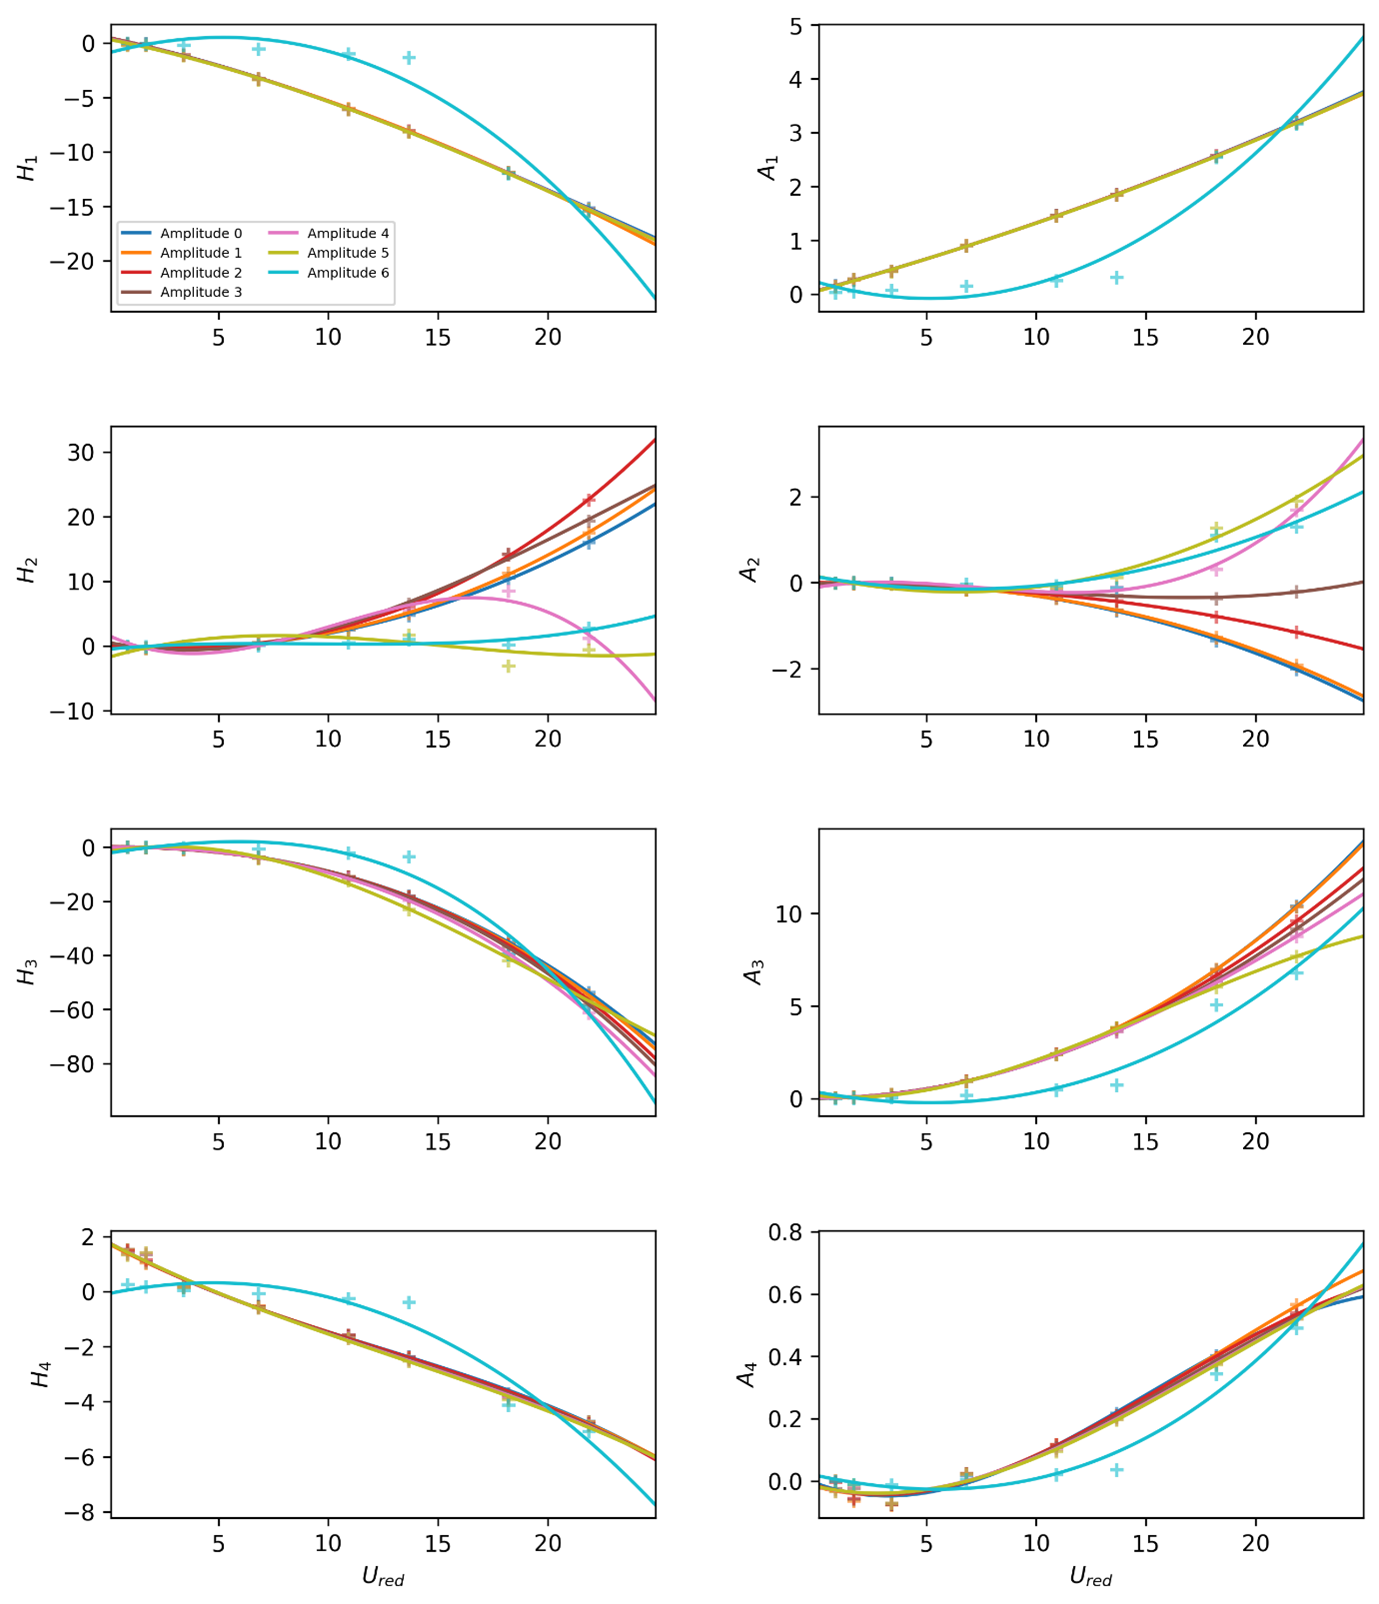
\includegraphics[width=1\textwidth]{Figures/Combined_Flutter_Derivative.png}
    \caption{Combined Flutter Derivatives}
    \label{fig:Combined_Flutter_Derivatives}
\end{figure}

\subsection{Spectral Analysis}

Spectral analysis is a powerful tool to identify the presence of nonlinear terms in the obtained forces and validating scanlan's linearity assumption. 
If the spectrum of the obtained forces contains higher-order sine terms other than applied frequency, 
then nonlinear behaviour is present. In this section, the spectrum of the obtained aerodynamic lift force and moment is analysed for different amplitudes. 
Discrete Fourier Transform (DFT) is used to obtain the spectrum of the obtained forces.
Plots of spectrum corresponding to the reduced velocity of 21.86 are shown, since this is the most affected by nonlinearity.\\

From Figure~\ref{fig:Frequency_Domain_Analysis_Heave} for all heave ampltiude range, the spectrum of the obtained both aerodynamic forces and moments are clean, 
indicating that the obtained forces are linear with respect to the prescribed motion.\\

From Figure~\ref{fig:Frequency_Domain_Analysis_Pitch}, for pitch amplitude up to 5 degrees for pitch, the spectrum of the obtained both aerodynamic forces and moments are clean, 
indicating that the obtained forces are linear with respect to the prescribed motion. Above these limits, significant noise is present, indicating the 
presence of higher-order sine terms and, therefore nonlinearity starts to appear. \\

On comparing Figure~\ref{fig:Combined_Flutter_Derivatives} and Figure~\ref{fig:Frequency_Domain_Analysis_Pitch}, 
it can be observed that the nonlinearity in flutter derivatives $A_2$ and $H_2$ starts to deviate at a lower pitch degree than the nonlinearity in the obtained spectrum analysis.
Hence this deviation in flutter derivatives is not due to nonlinearity in the obtained forces. Though it validates the thumb rule of 5 degrees for pitch motion, 
it raises the question of why the flutter derivatives show nonlinearity at a lower pitch degree than the obtained forces.\\

\begin{figure}[htbp]  
    \centering
    \begin{subfigure}[b]{0.45\textwidth}
        \centering
        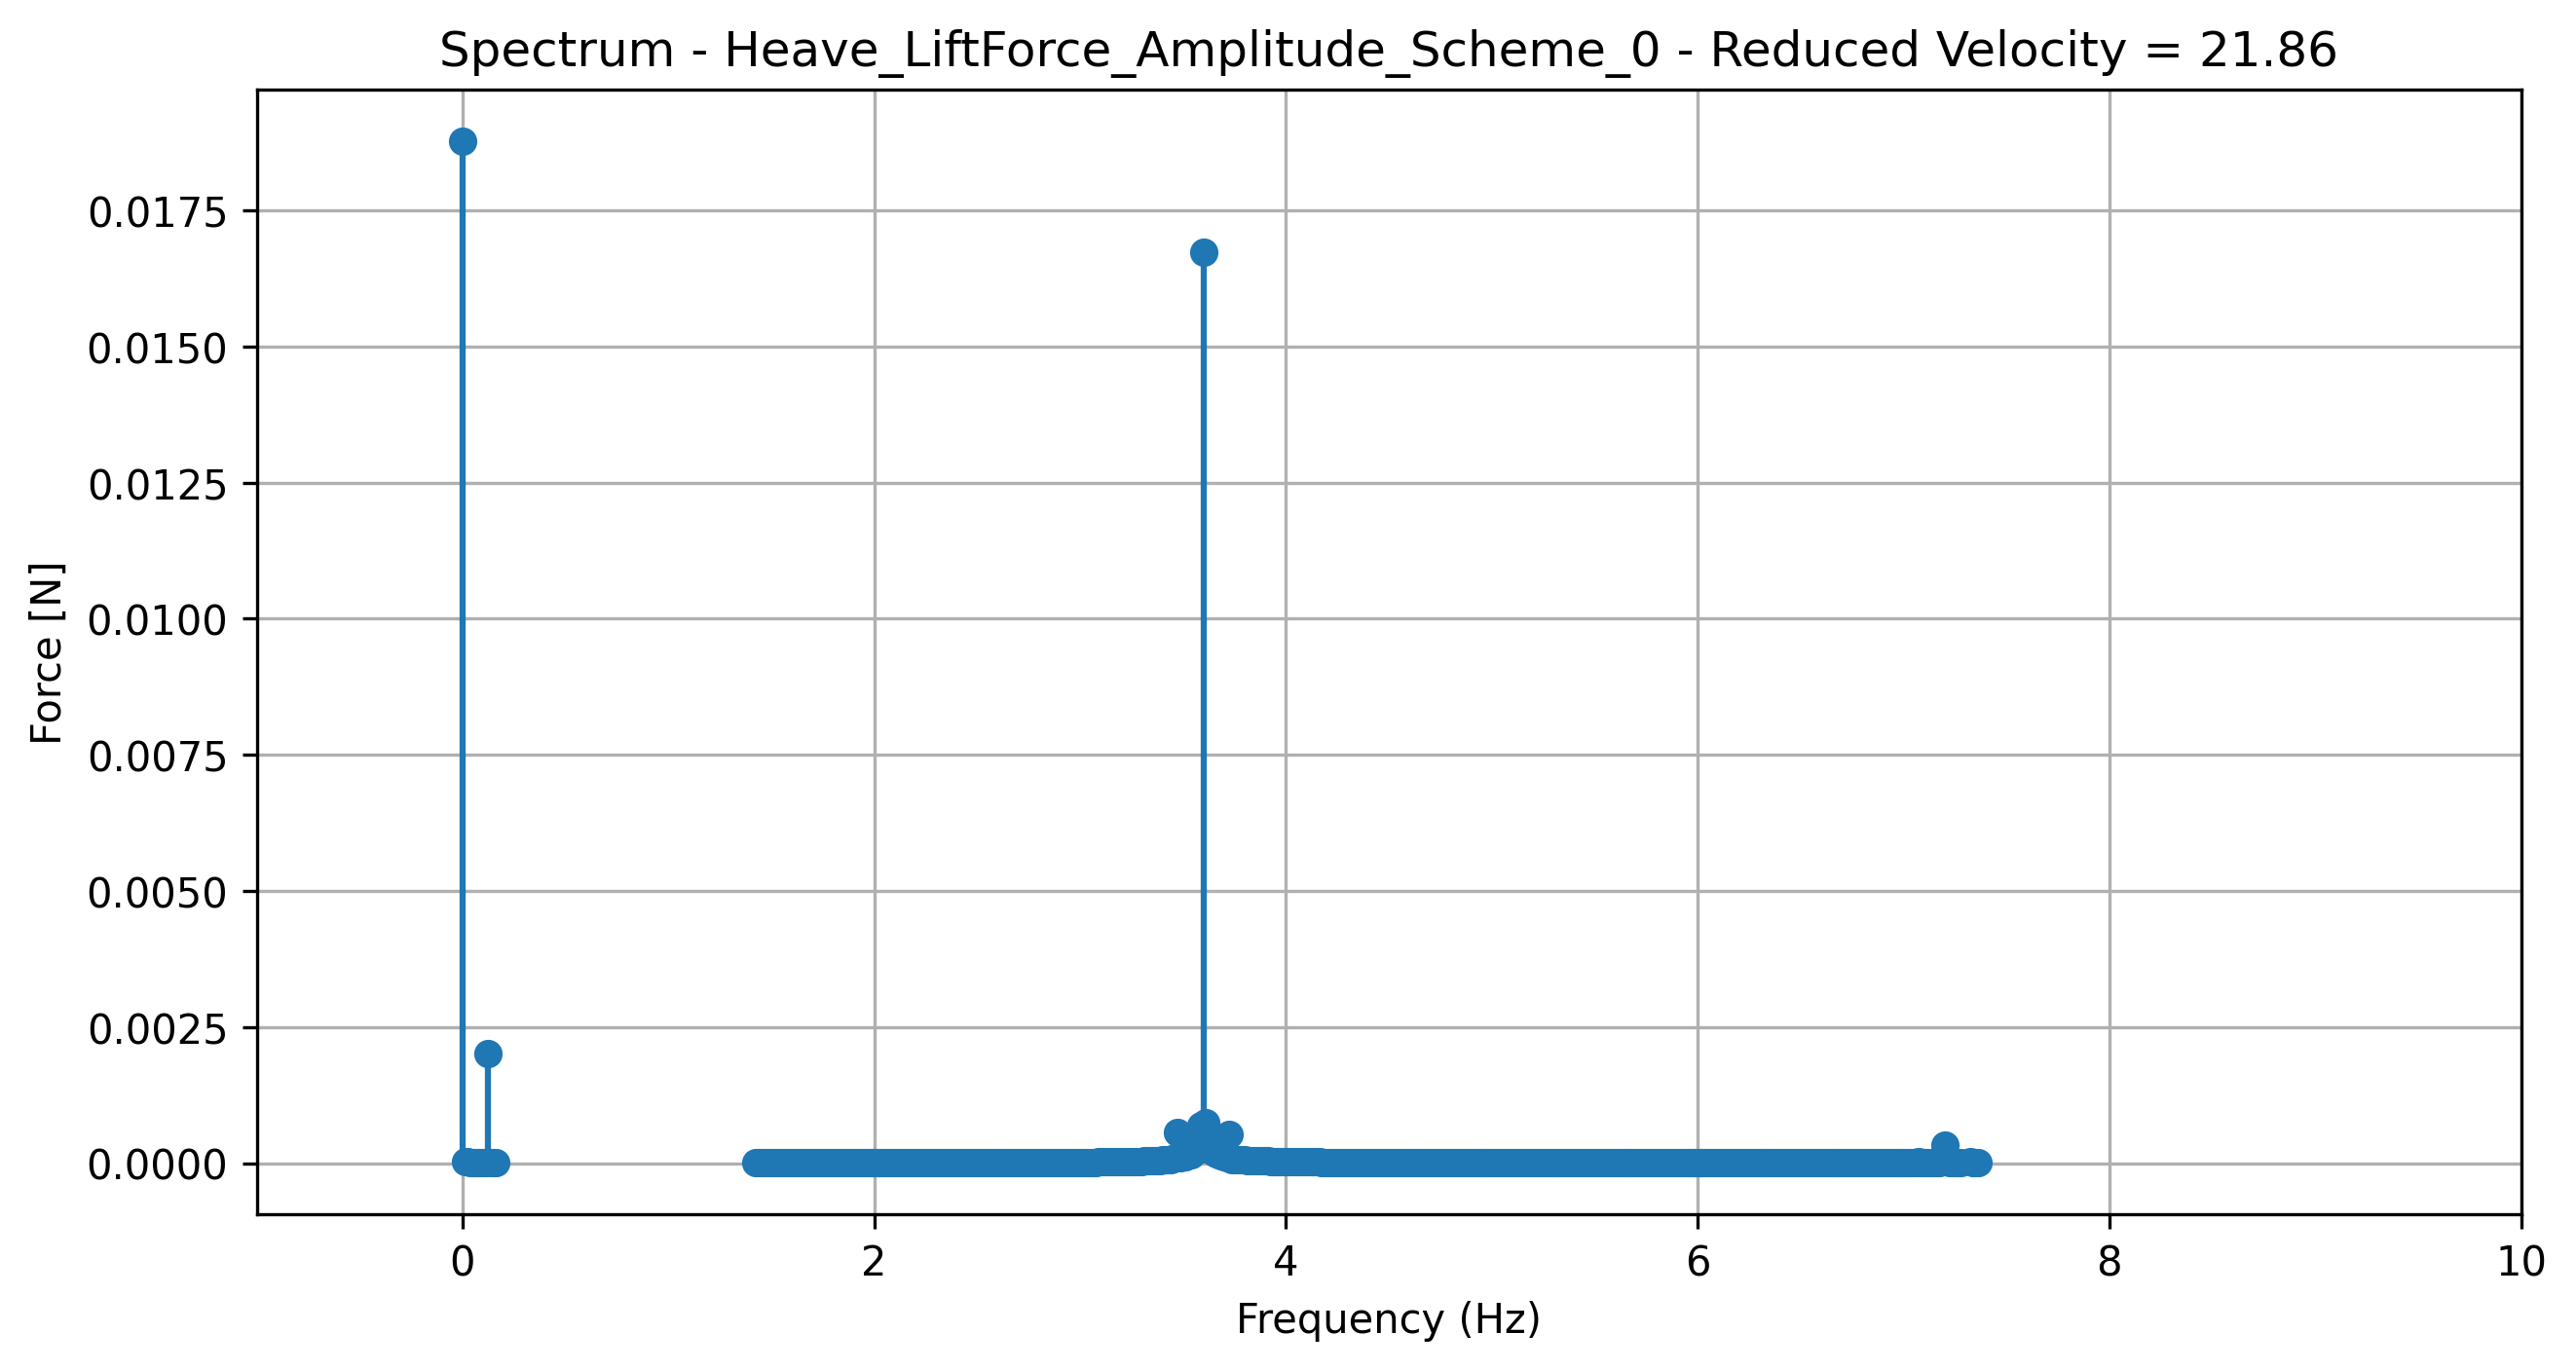
\includegraphics[width=\textwidth]{Figures/Frequency_Domain_Analysis/Heave/DFT_LiftForce_Amplitude_Scheme_0.png}
        \caption{}
        \label{fig:Heave_DFT_Fy_amplitude_Scheme_0}
    \end{subfigure}
    \hfill
    \begin{subfigure}[b]{0.45\textwidth}
        \centering
        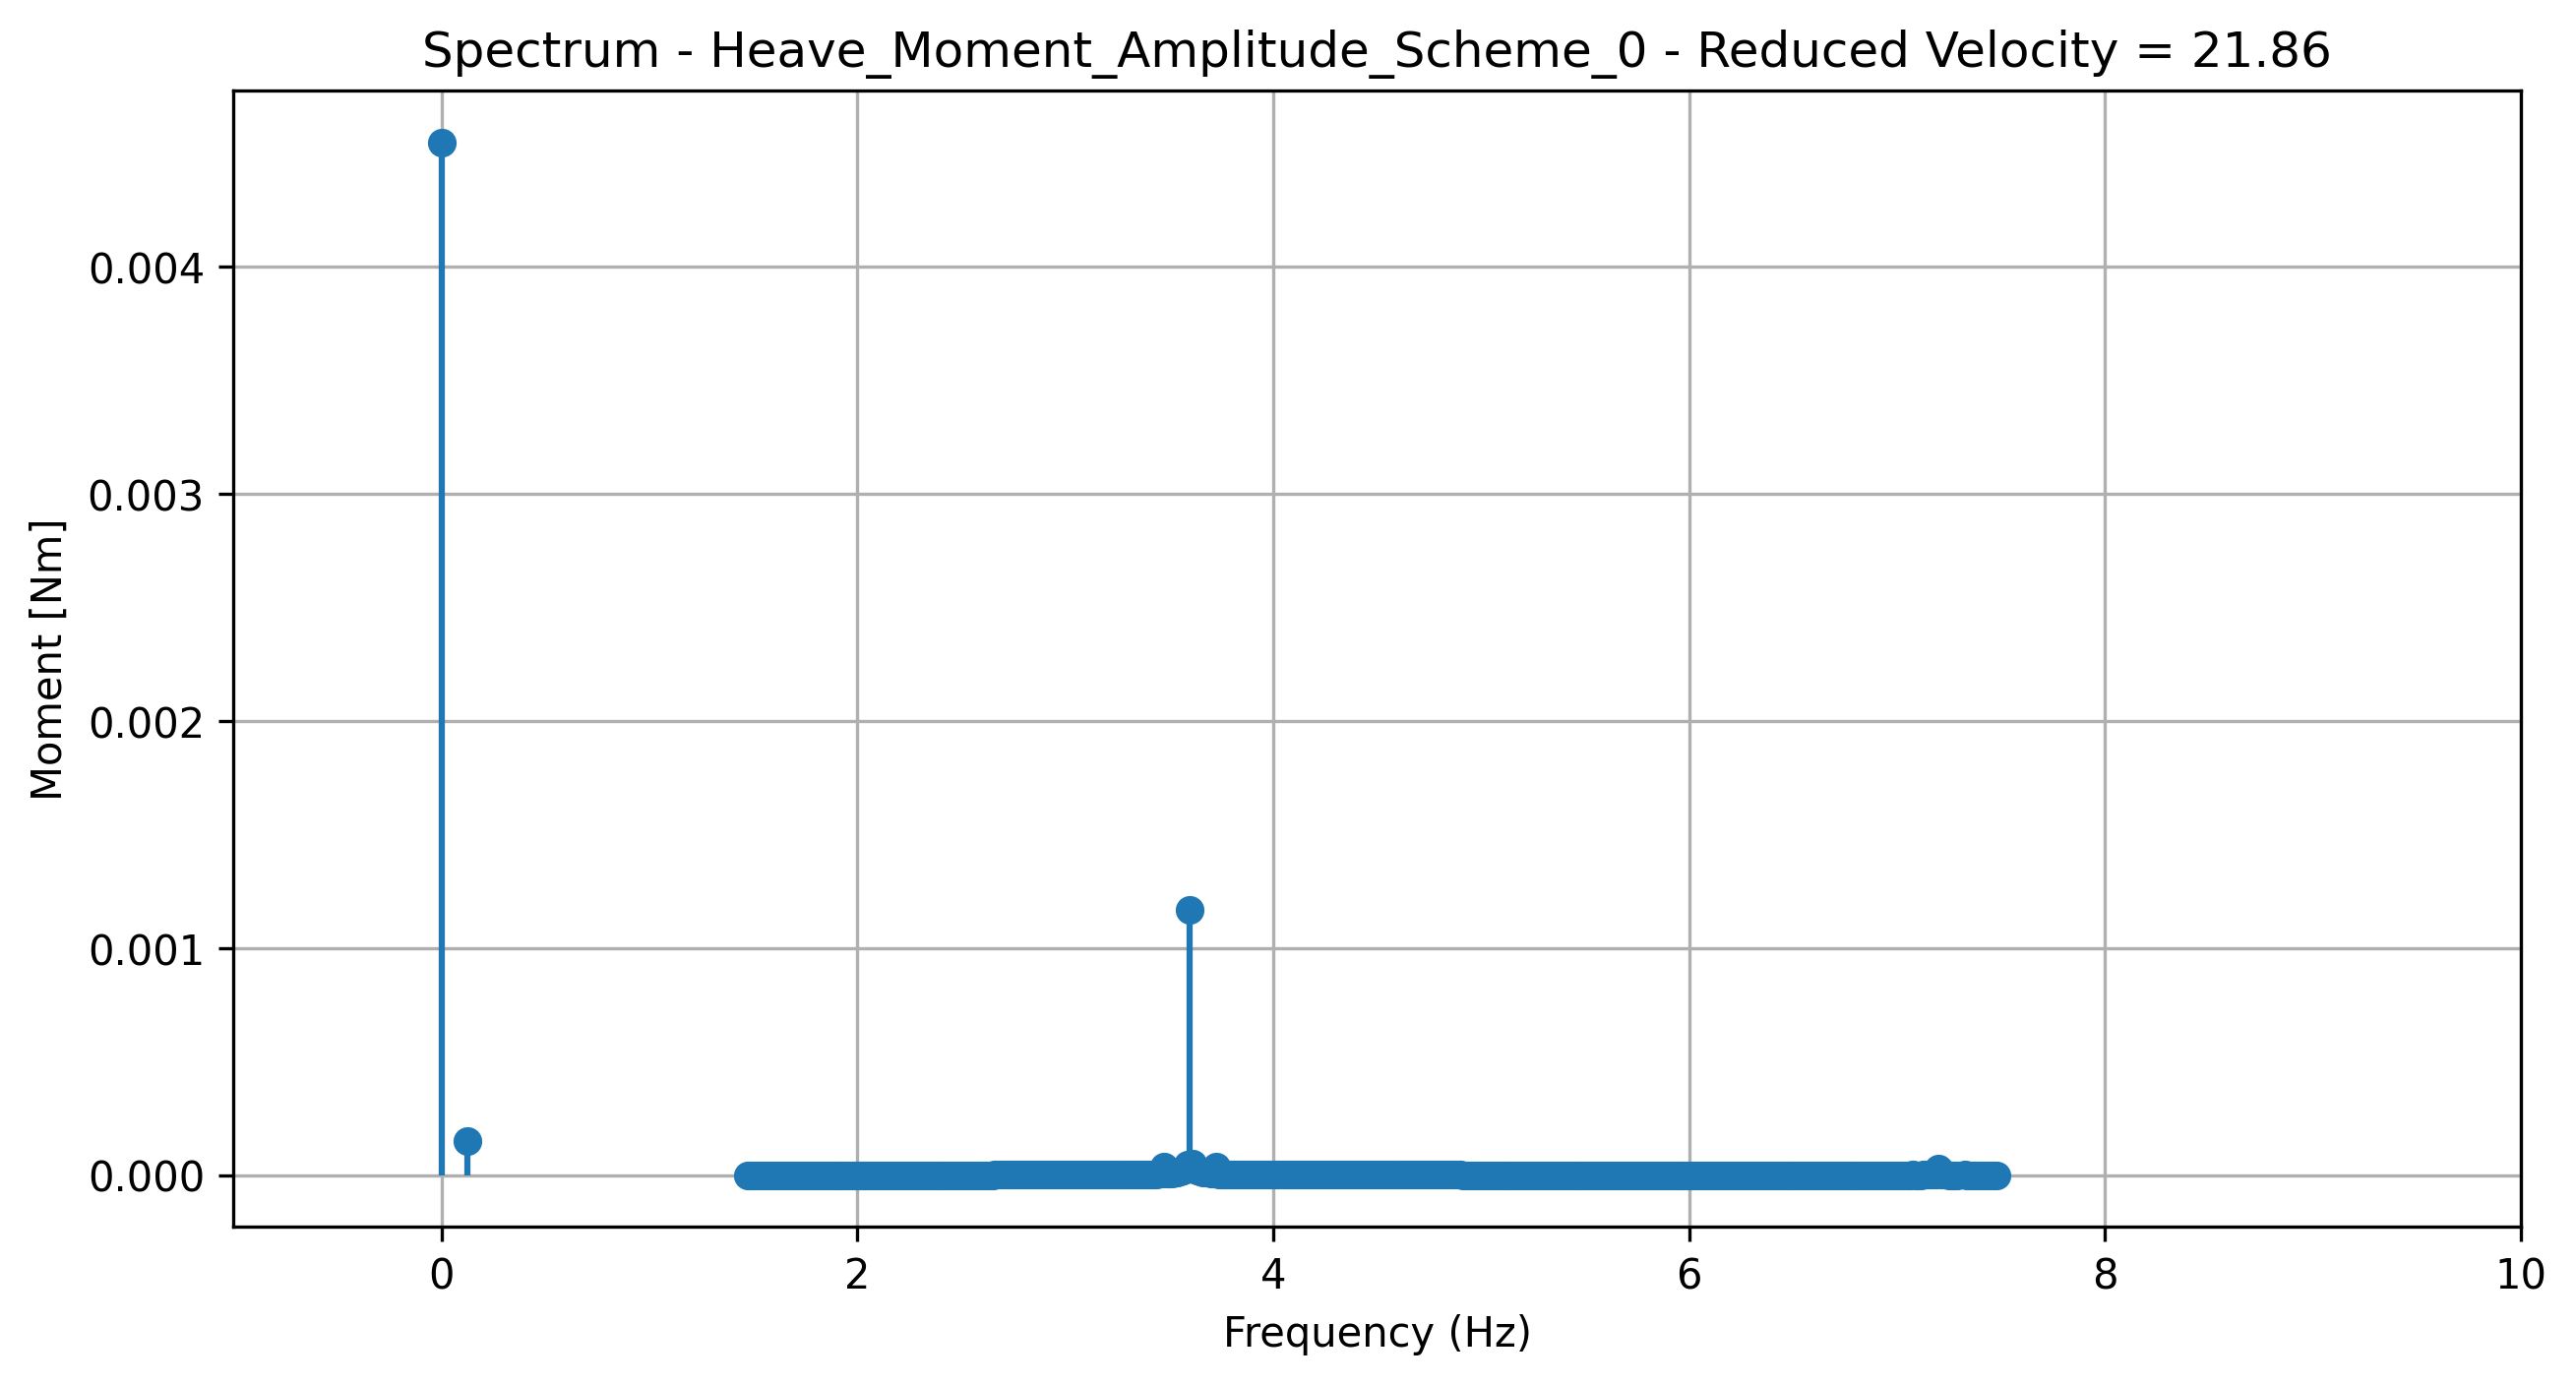
\includegraphics[width=\textwidth]{Figures/Frequency_Domain_Analysis/Heave/DFT_Moment_Amplitude_Scheme_0.png}
        \caption{}
        \label{fig:Heave_DFT_moment_amplitude_Scheme_0}
    \end{subfigure}
    
    % \begin{subfigure}[b]{0.45\textwidth}
    %     \centering
    %     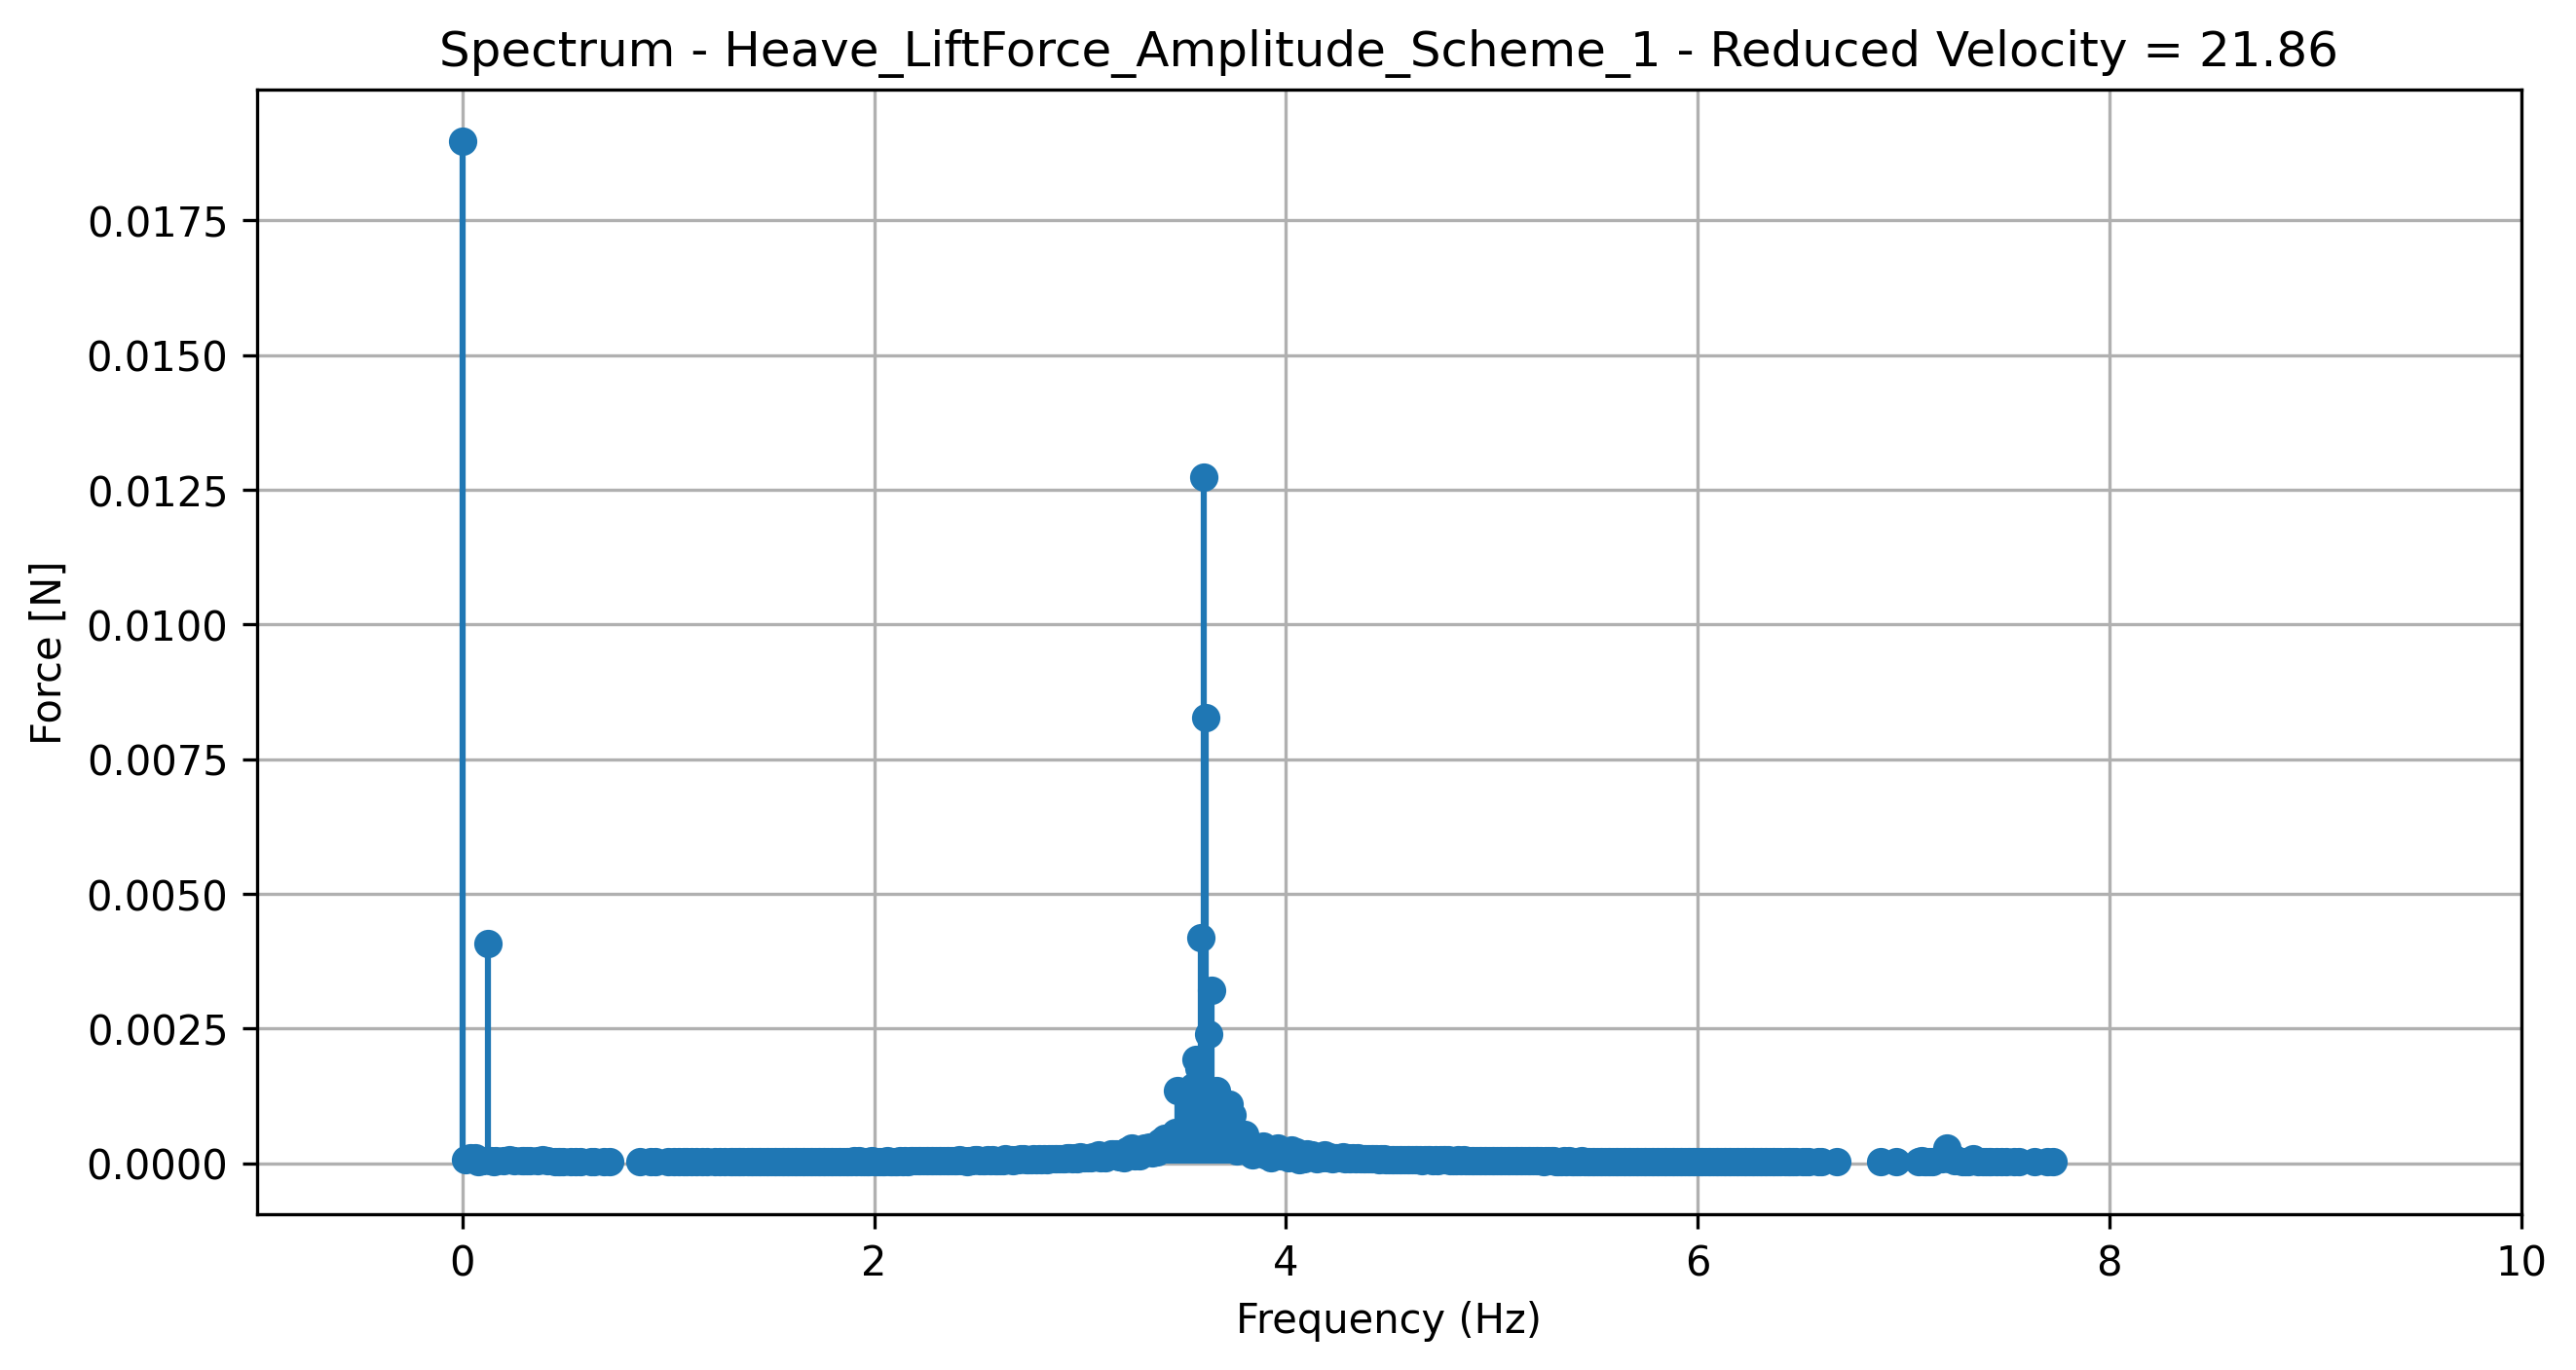
\includegraphics[width=\textwidth]{Figures/Frequency_Domain_Analysis/Heave/DFT_LiftForce_Amplitude_Scheme_1.png}
    %     \caption{}
    %     \label{fig:Heave_DFT_Fy_amplitude_Scheme_1}
    % \end{subfigure}
    % \hfill
    % \begin{subfigure}[b]{0.45\textwidth}
    %     \centering
    %     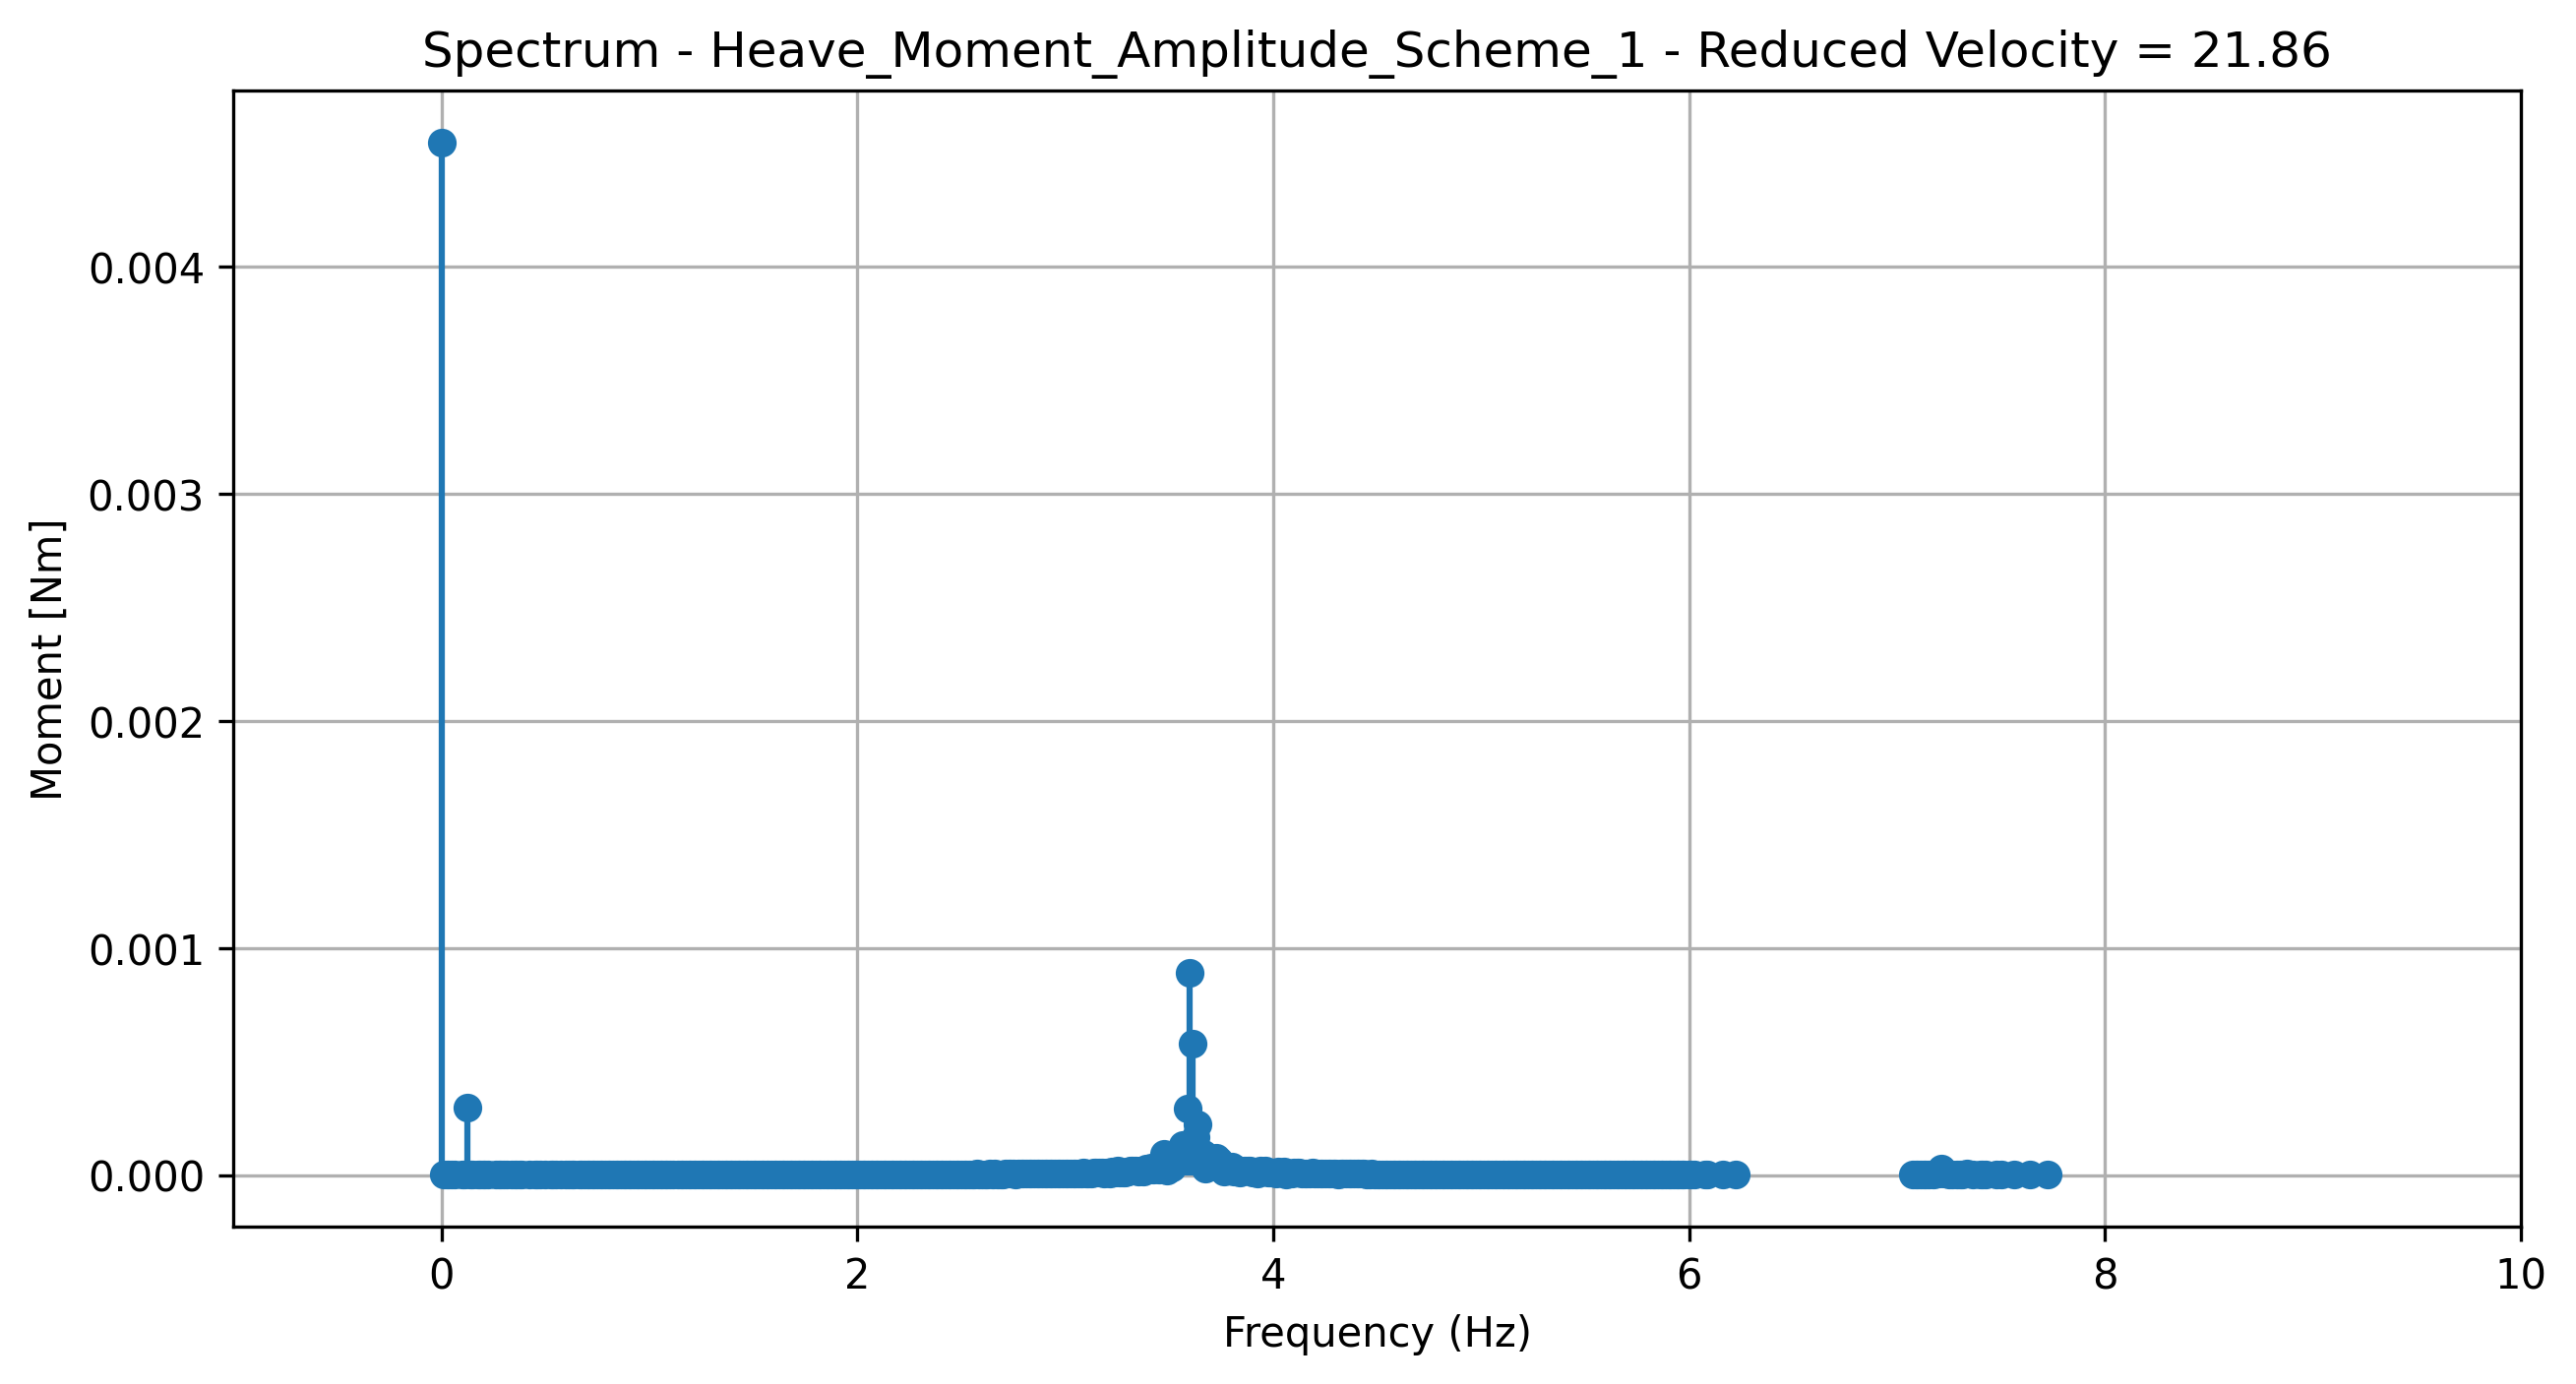
\includegraphics[width=\textwidth]{Figures/Frequency_Domain_Analysis/Heave/DFT_Moment_Amplitude_Scheme_1.png}
    %     \caption{}
    %     \label{fig:Heave_DFT_moment_amplitude_Scheme_1}
    % \end{subfigure}
    
    \begin{subfigure}[b]{0.45\textwidth}
        \centering
        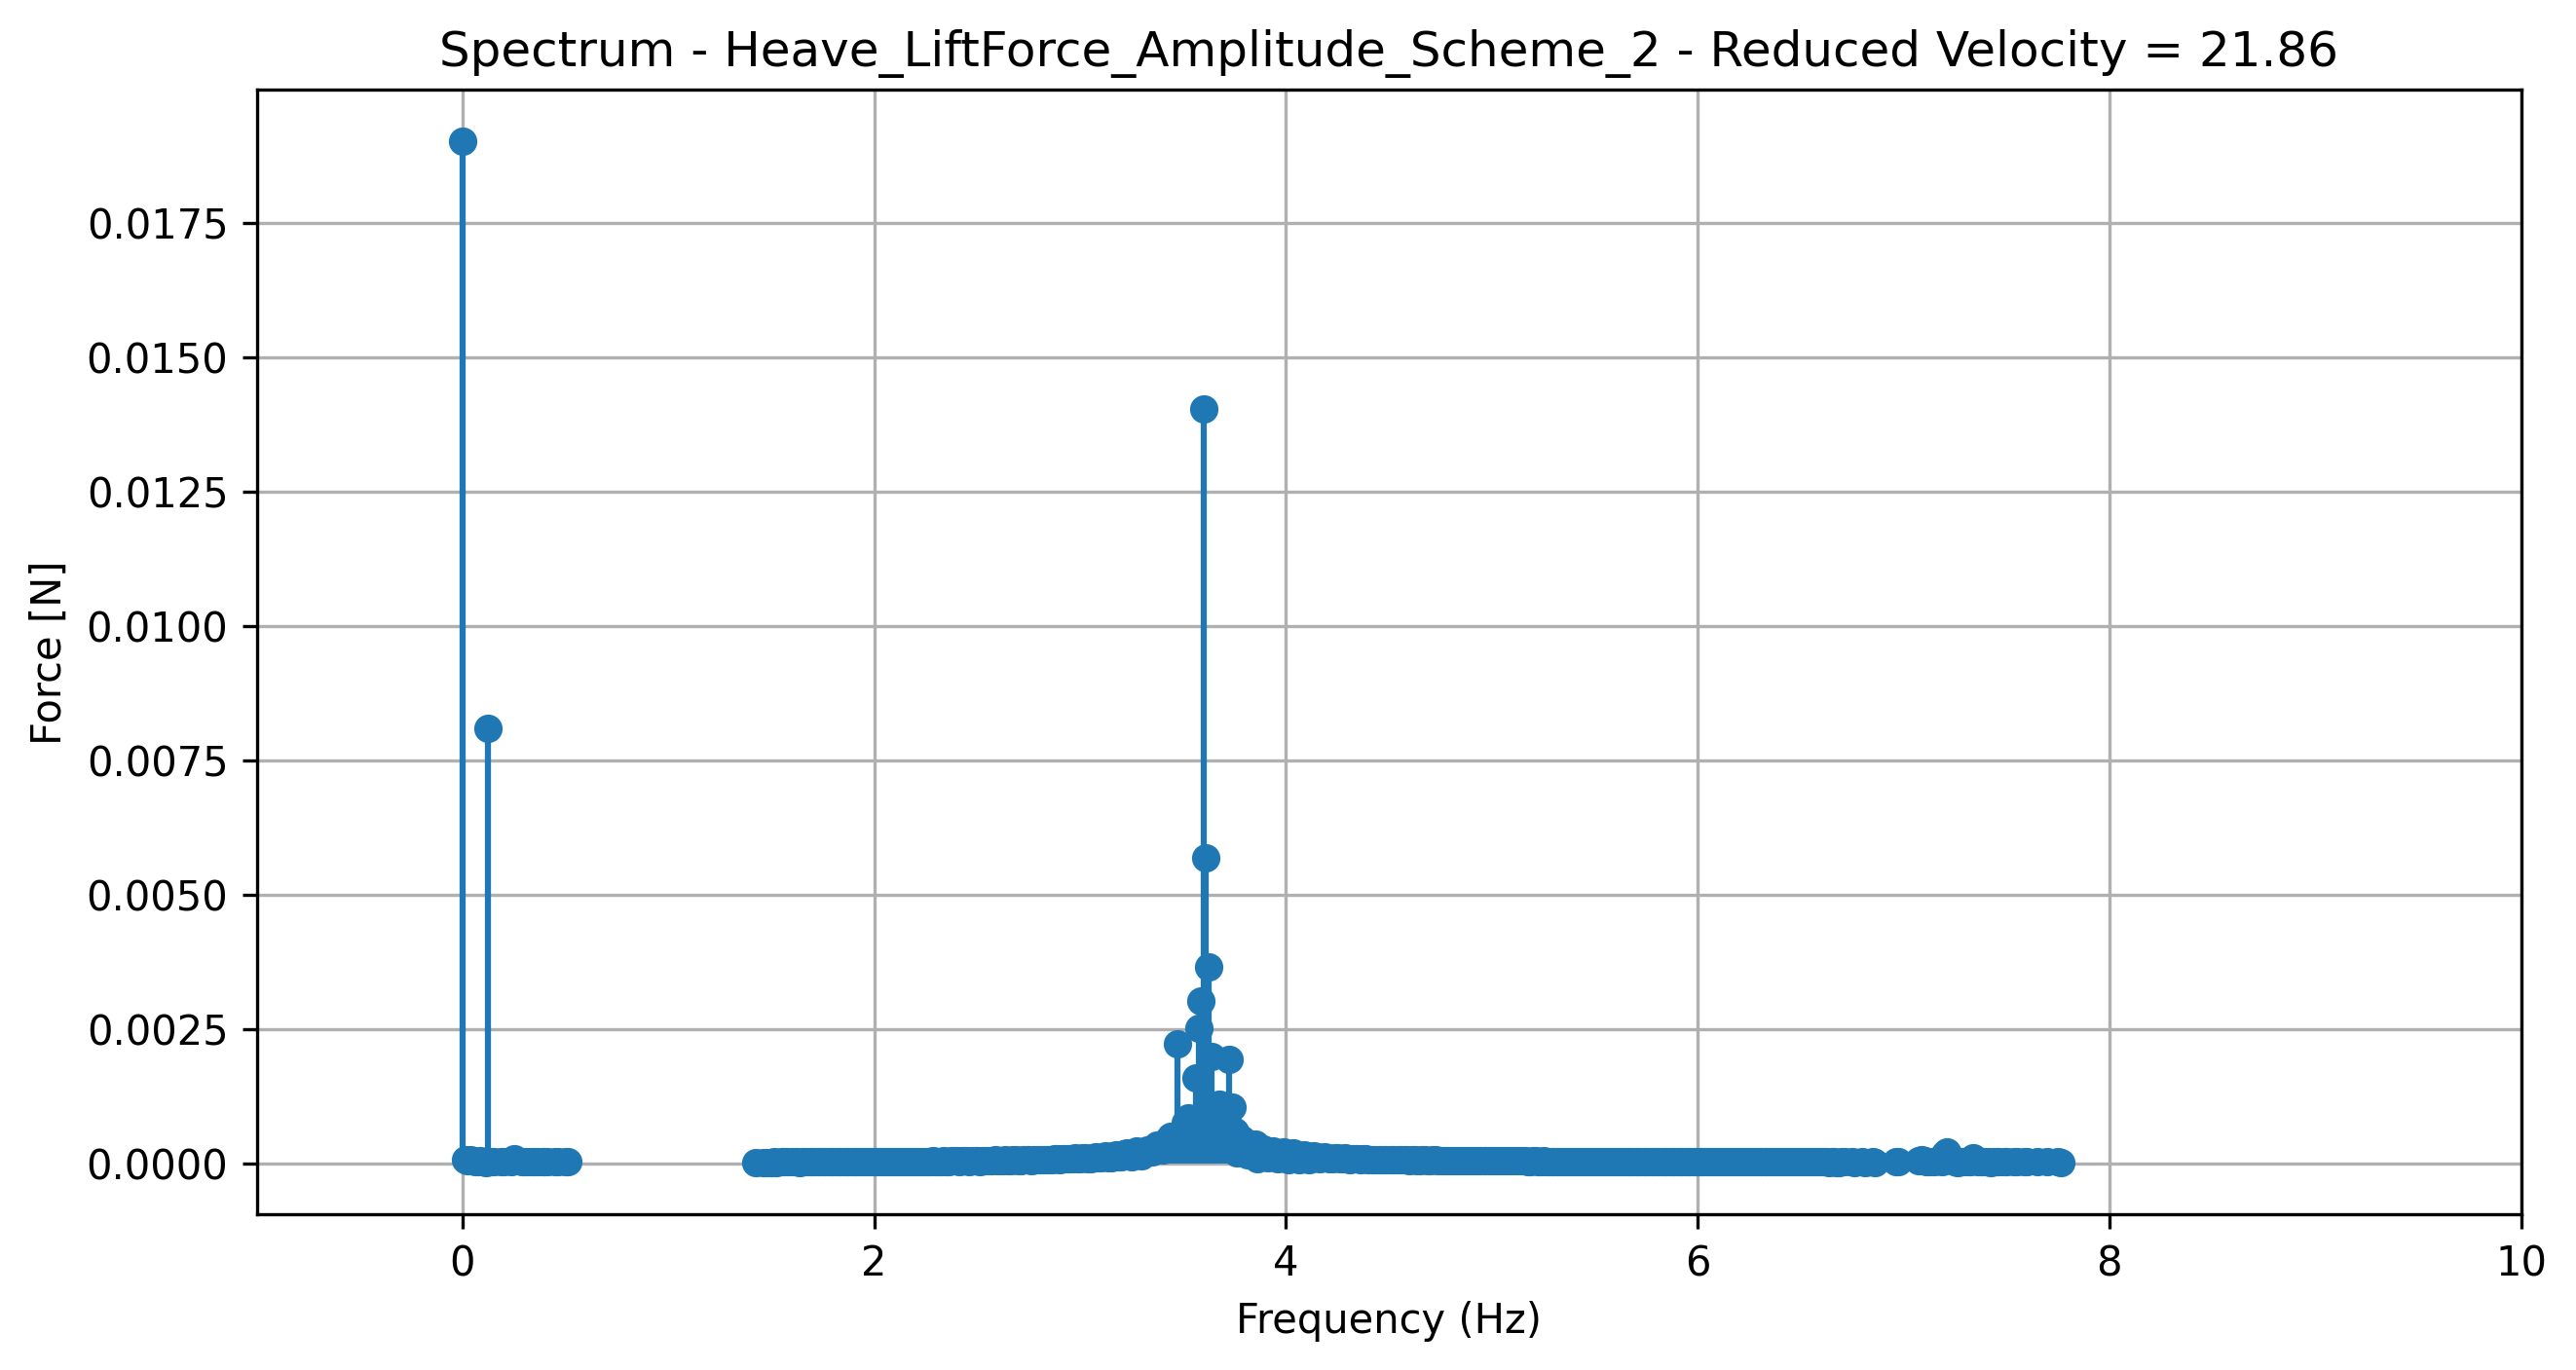
\includegraphics[width=\textwidth]{Figures/Frequency_Domain_Analysis/Heave/DFT_LiftForce_Amplitude_Scheme_2.png}
        \caption{}
        \label{fig:Heave_DFT_Fy_amplitude_Scheme_2}
    \end{subfigure}
    \hfill
    \begin{subfigure}[b]{0.45\textwidth}
        \centering
        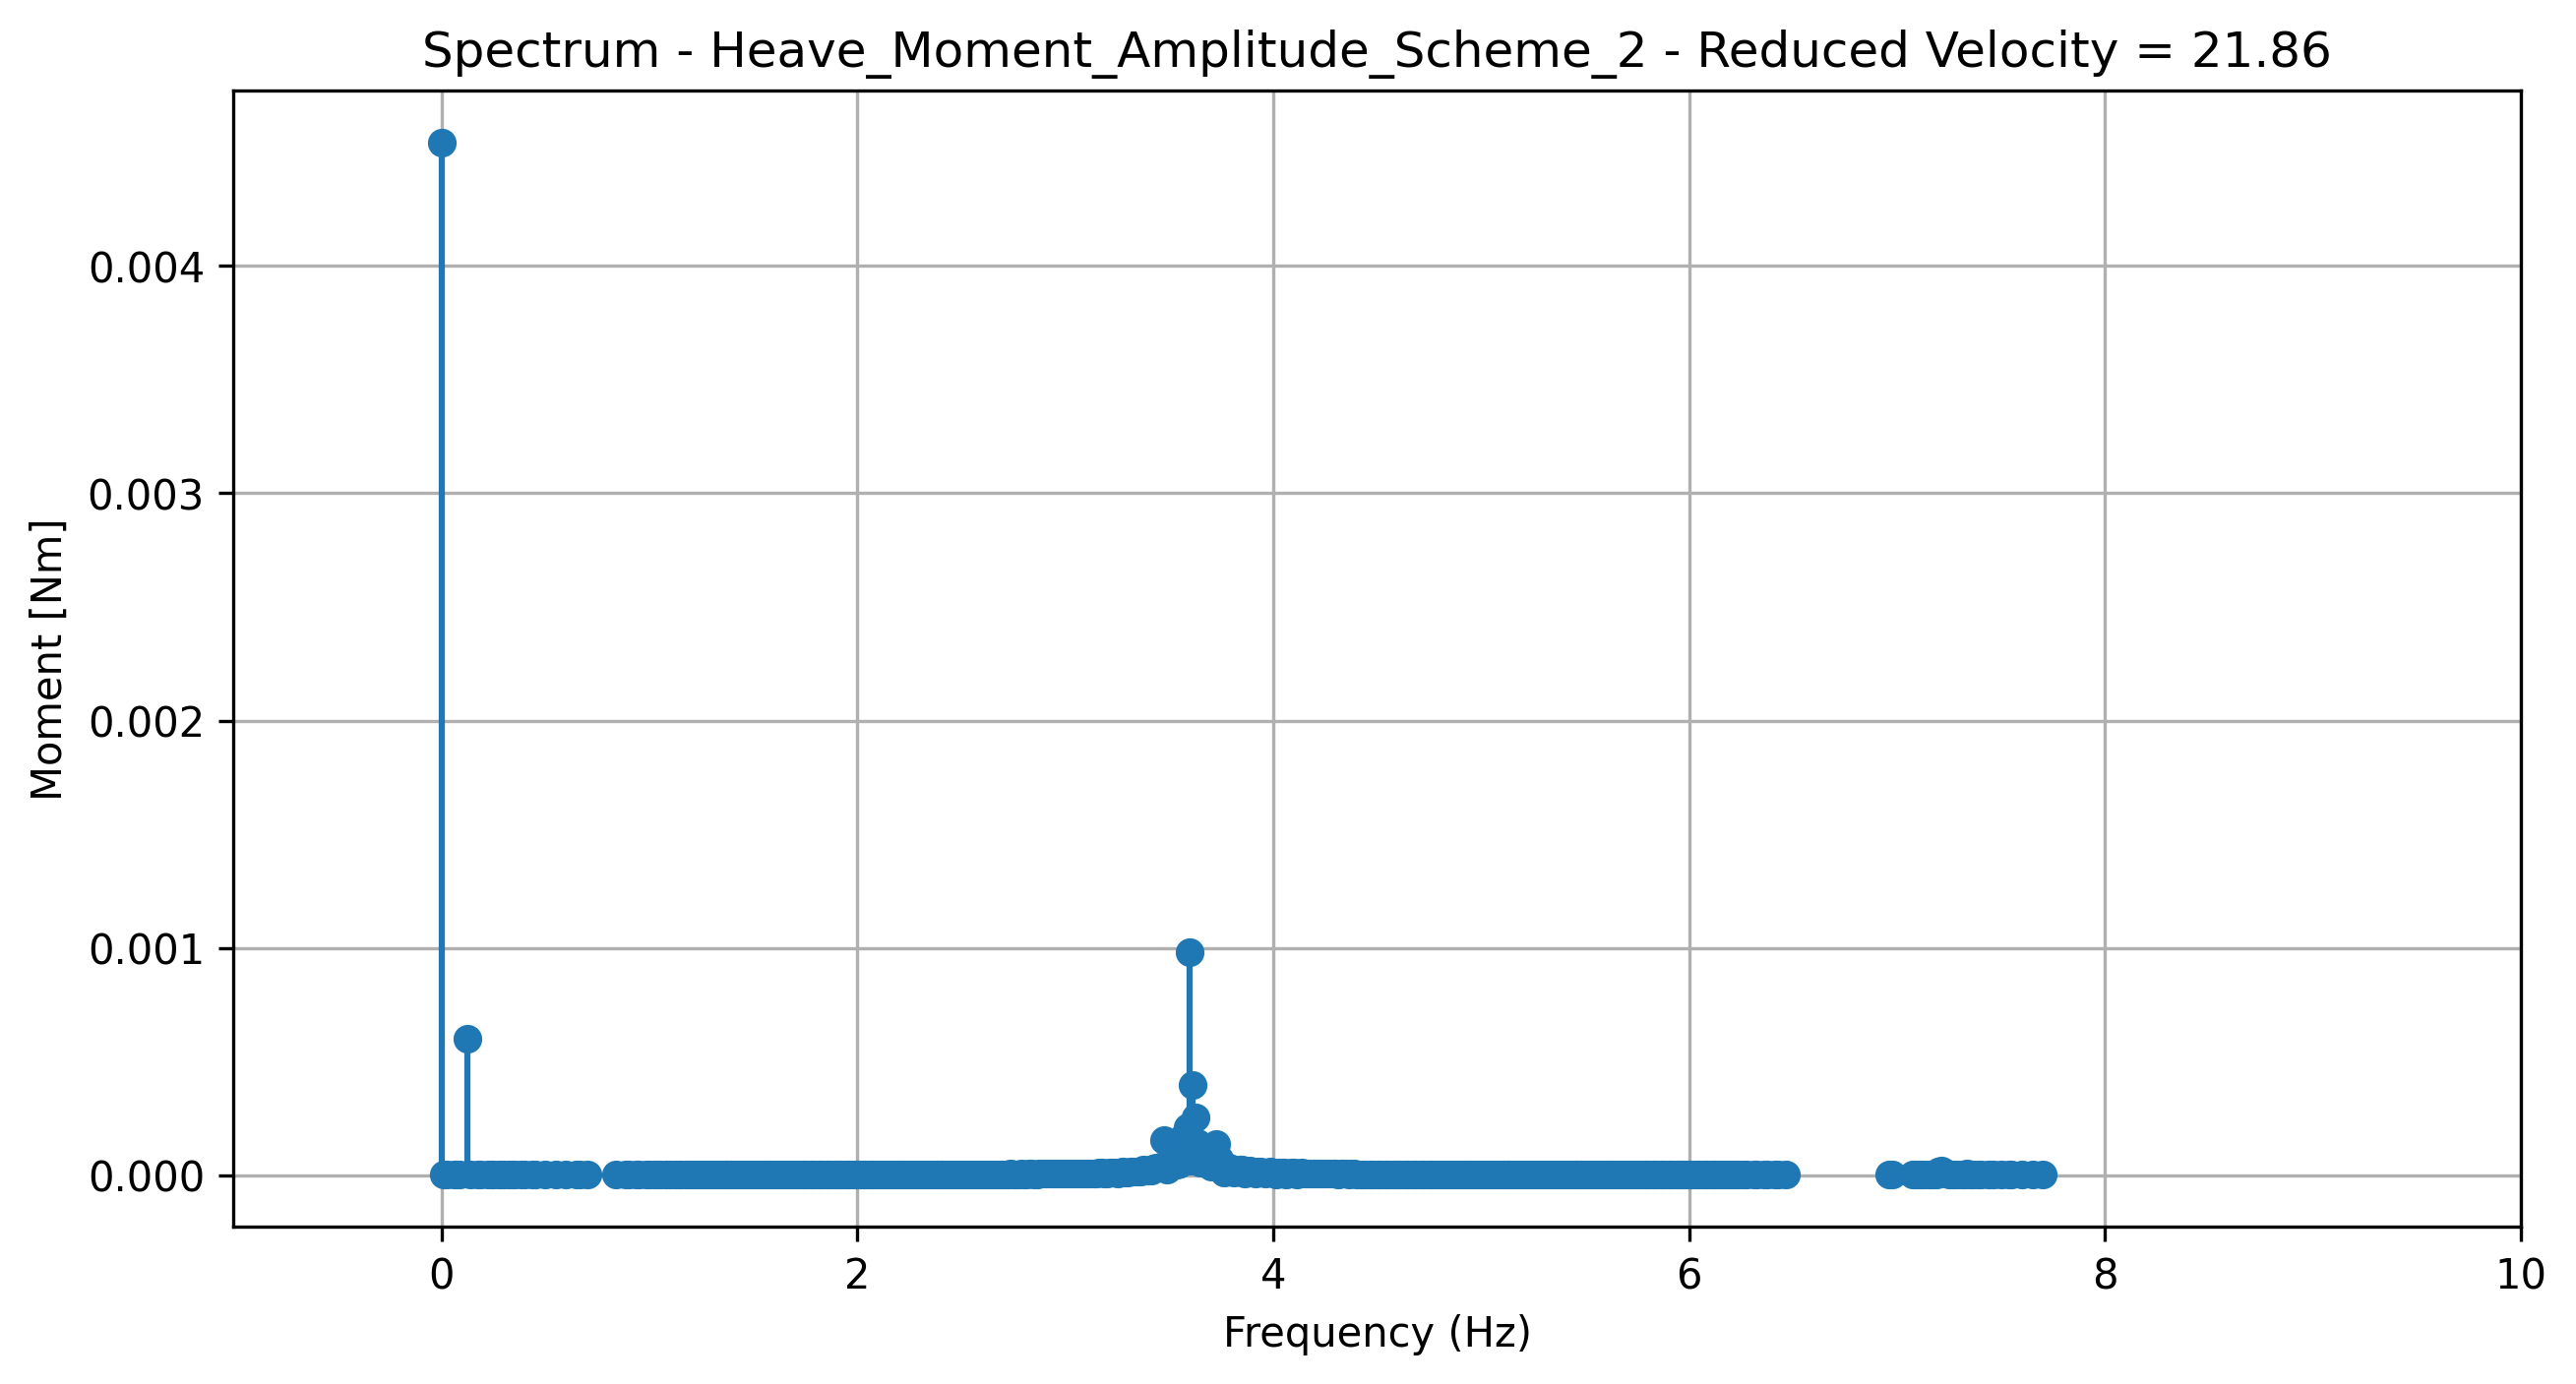
\includegraphics[width=\textwidth]{Figures/Frequency_Domain_Analysis/Heave/DFT_Moment_Amplitude_Scheme_2.png}
        \caption{}
        \label{fig:Heave_DFT_moment_amplitude_Scheme_2}
    \end{subfigure}
    
    \begin{subfigure}[b]{0.45\textwidth}
        \centering
        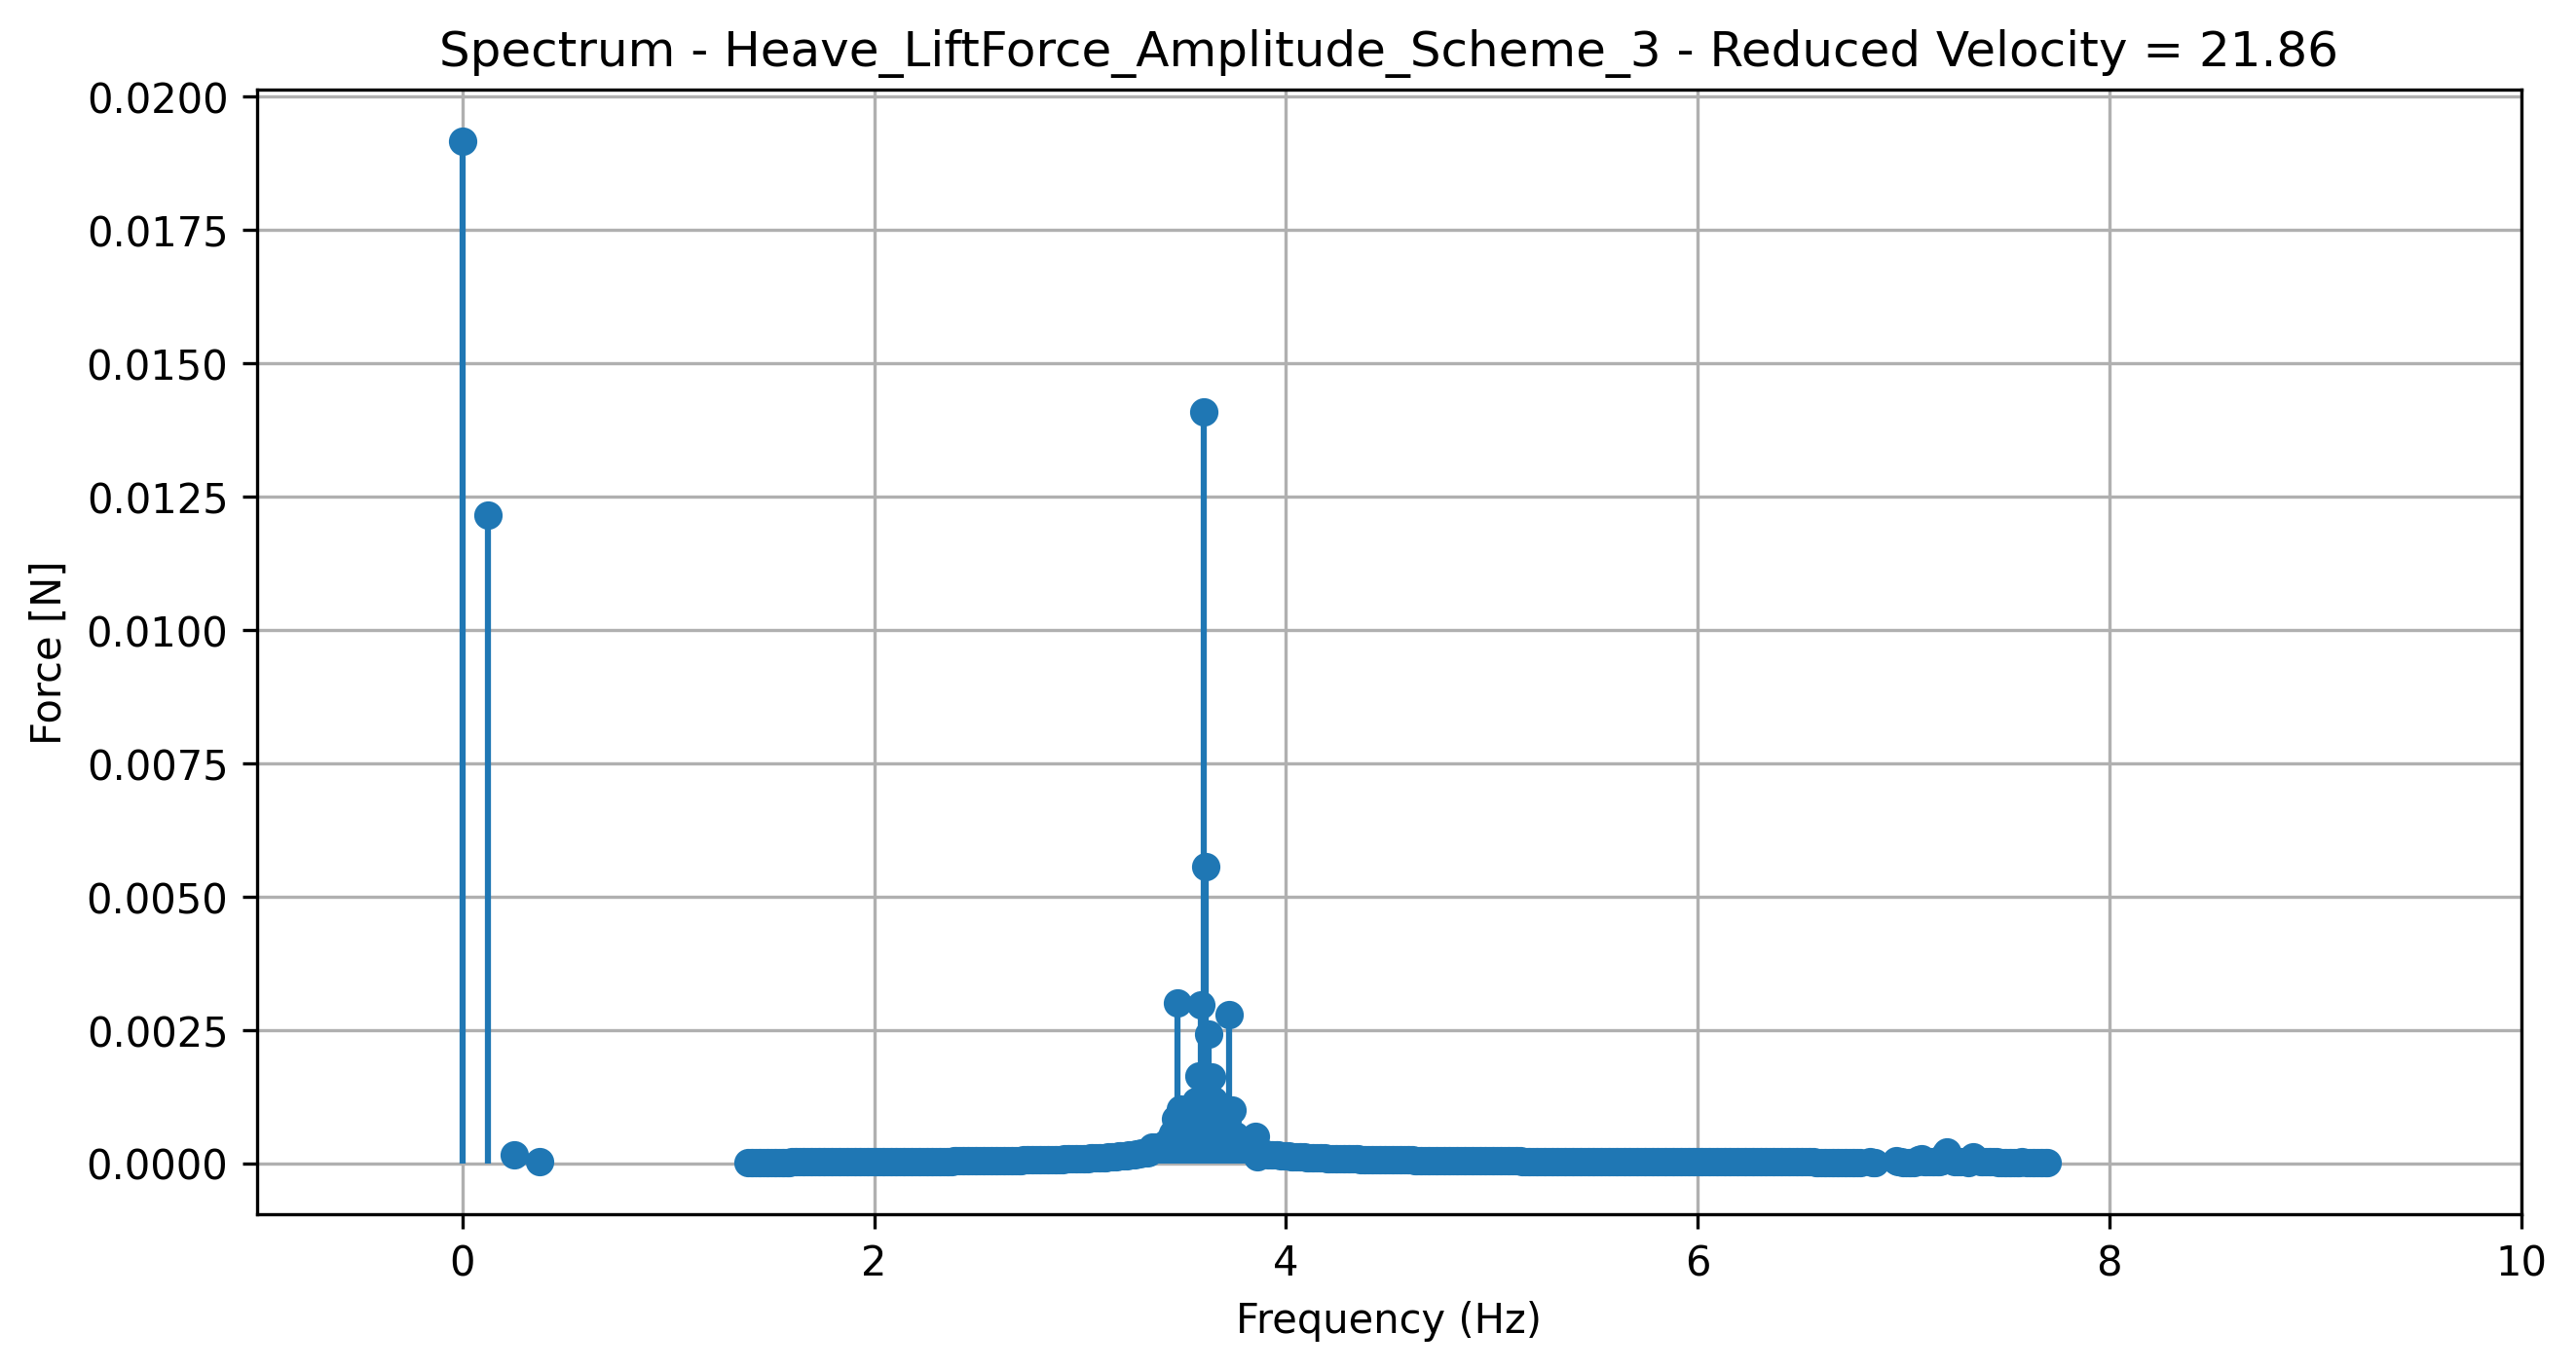
\includegraphics[width=\textwidth]{Figures/Frequency_Domain_Analysis/Heave/DFT_LiftForce_Amplitude_Scheme_3.png}
        \caption{}
        \label{fig:Heave_DFT_Fy_amplitude_Scheme_3}
    \end{subfigure}
    \hfill
    \begin{subfigure}[b]{0.45\textwidth}
        \centering
        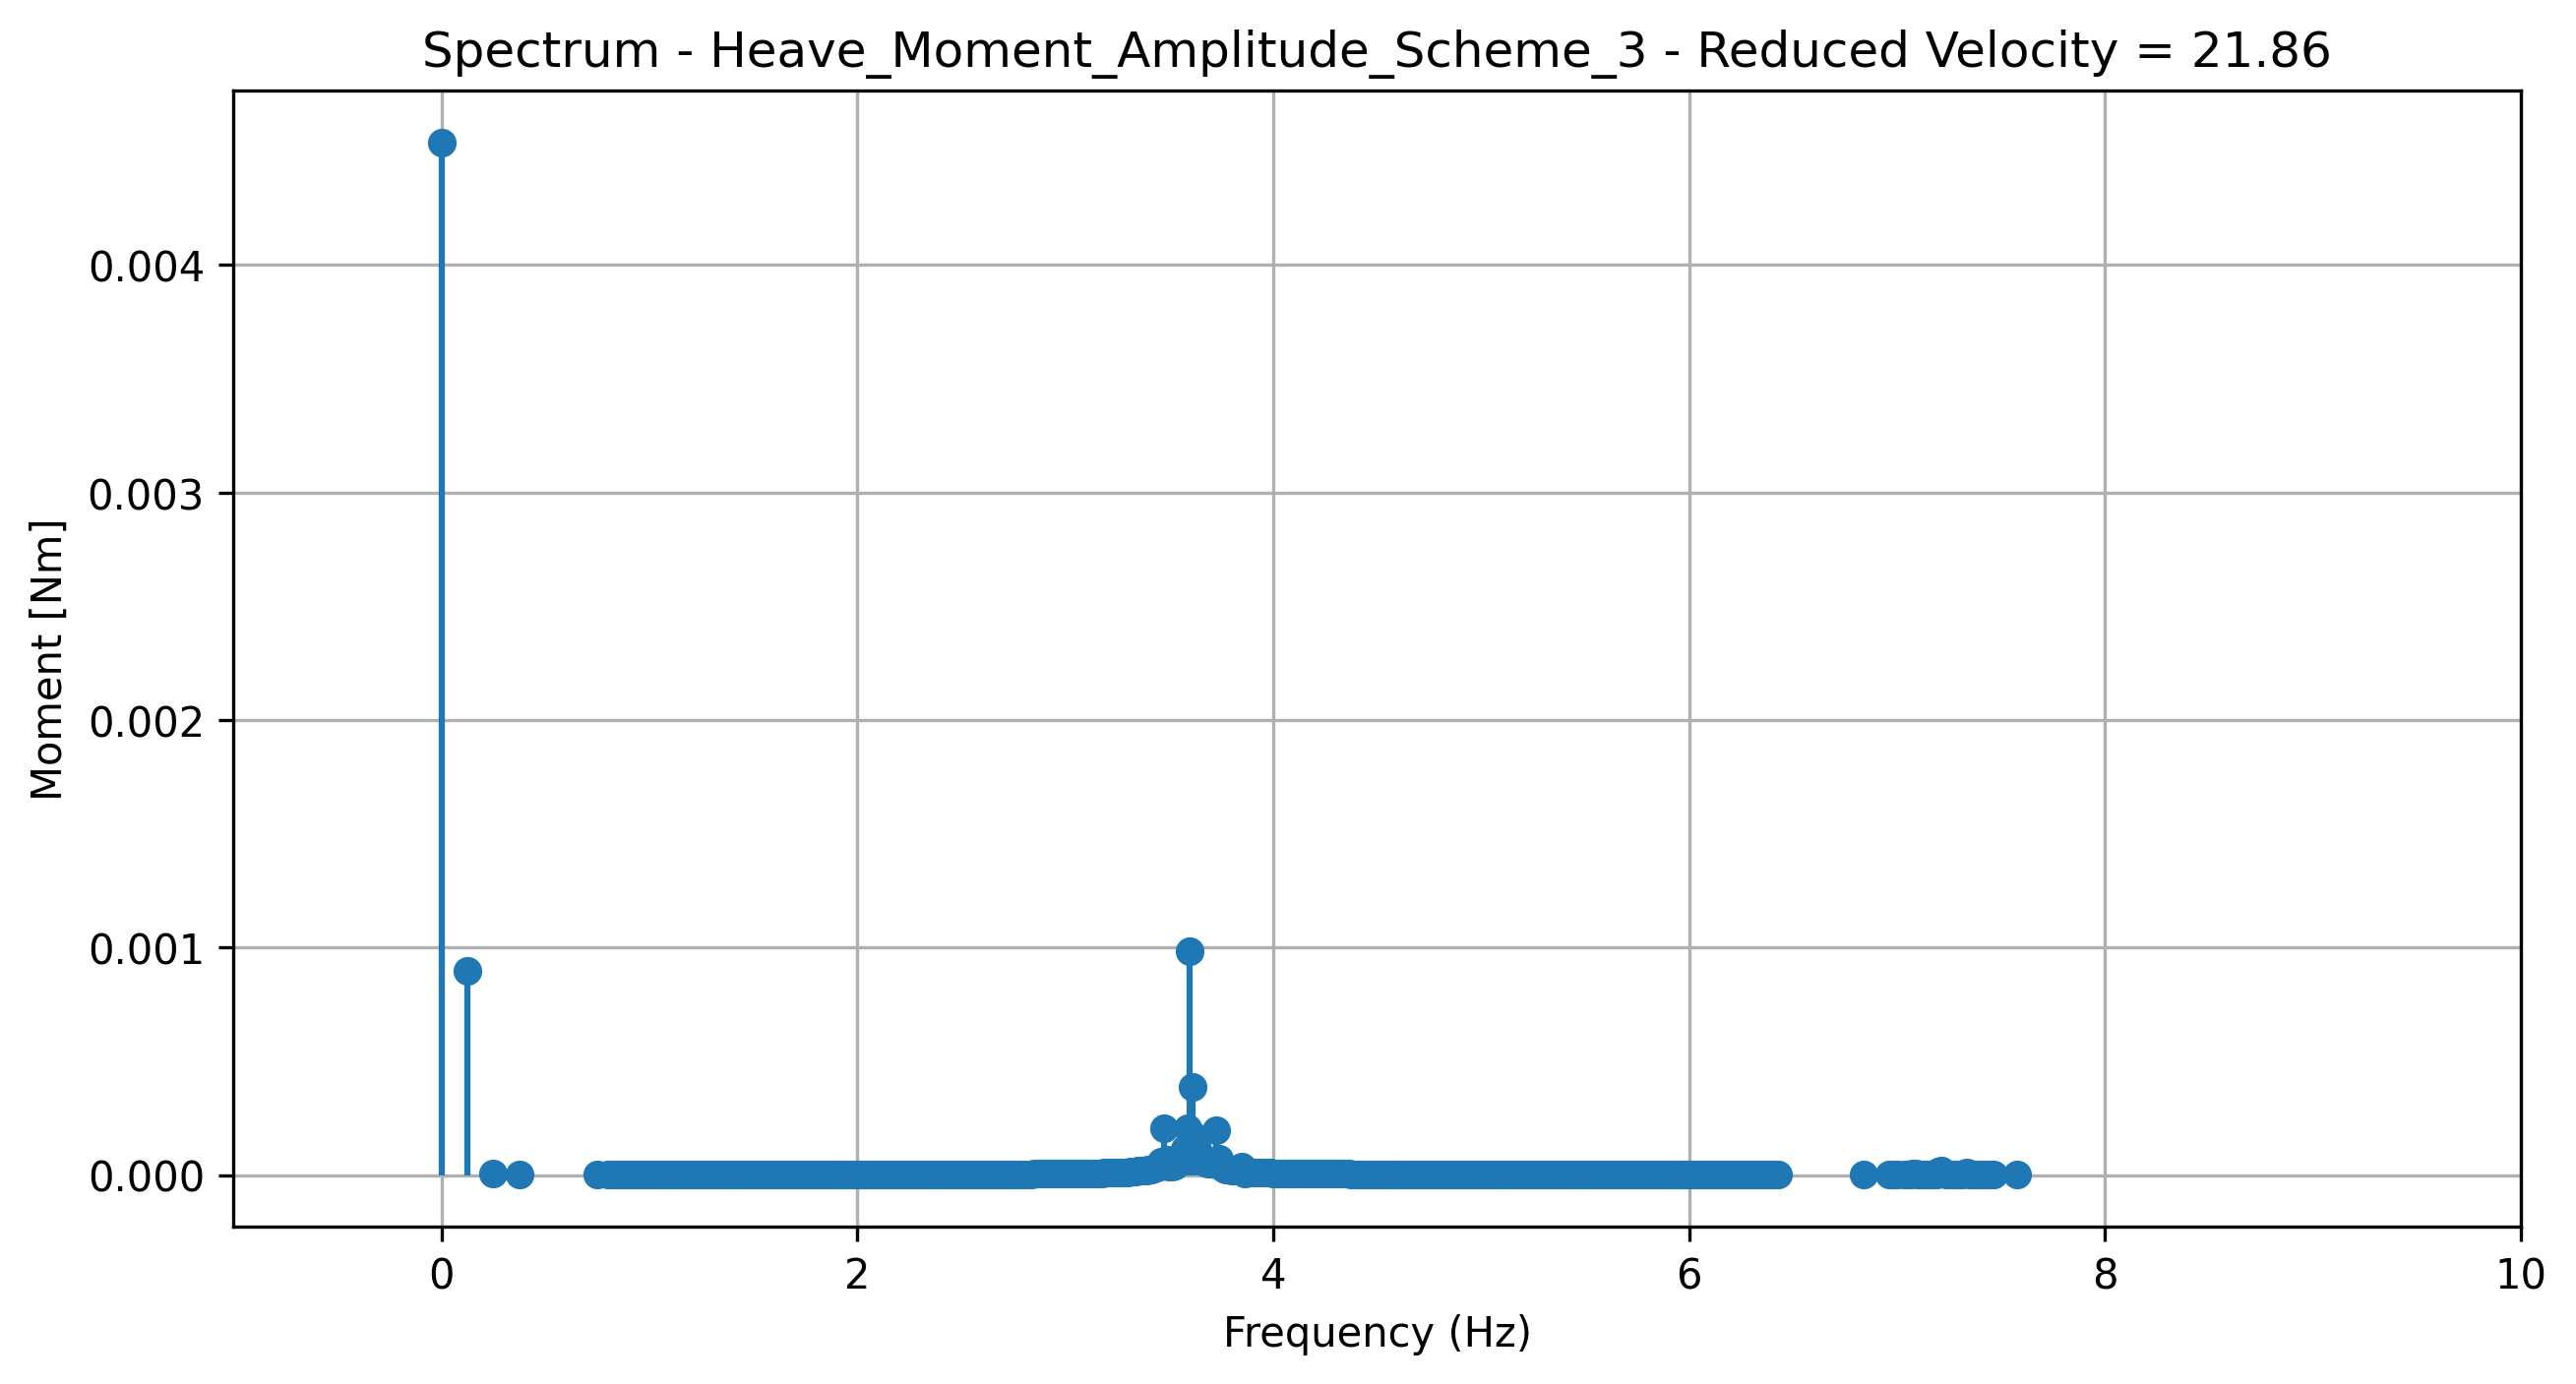
\includegraphics[width=\textwidth]{Figures/Frequency_Domain_Analysis/Heave/DFT_Moment_Amplitude_Scheme_3.png}
        \caption{}
        \label{fig:Heave_DFT_moment_amplitude_Scheme_3}
    \end{subfigure}

    \begin{subfigure}[b]{0.45\textwidth}
        \centering
        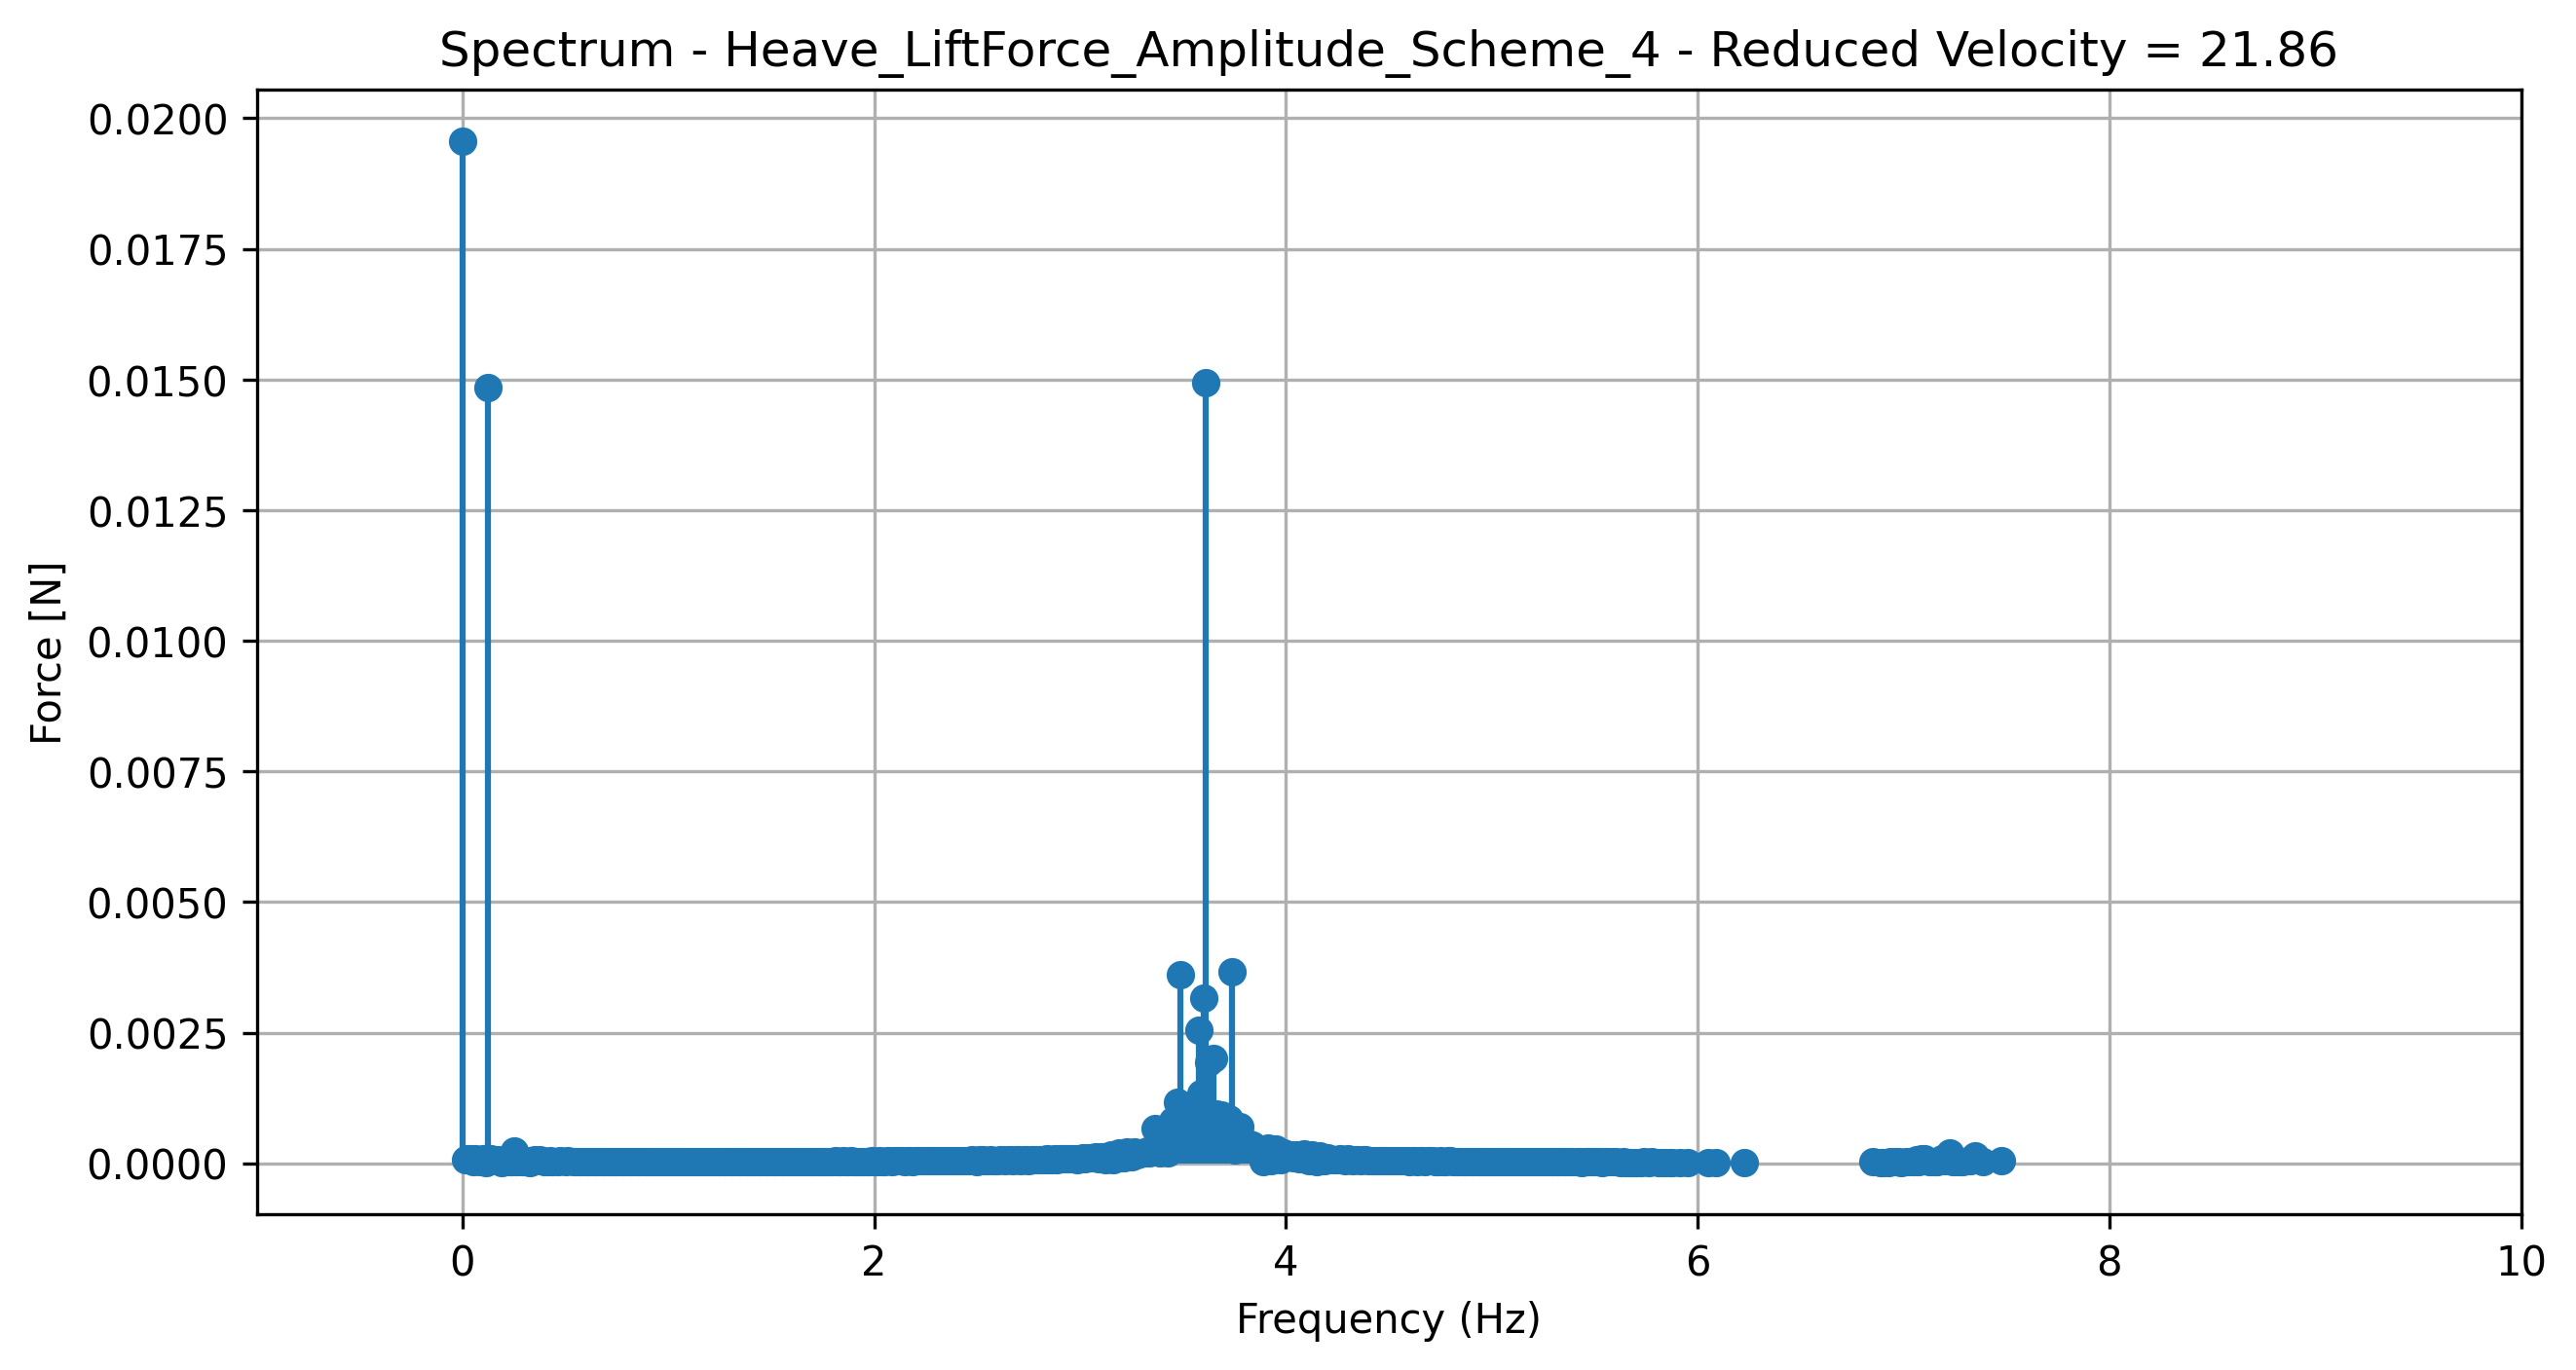
\includegraphics[width=\textwidth]{Figures/Frequency_Domain_Analysis/Heave/DFT_LiftForce_Amplitude_Scheme_4.png}
        \caption{}
        \label{fig:Heave_DFT_Fy_amplitude_Scheme_4}
    \end{subfigure}
    \hfill
    \begin{subfigure}[b]{0.45\textwidth}
        \centering
        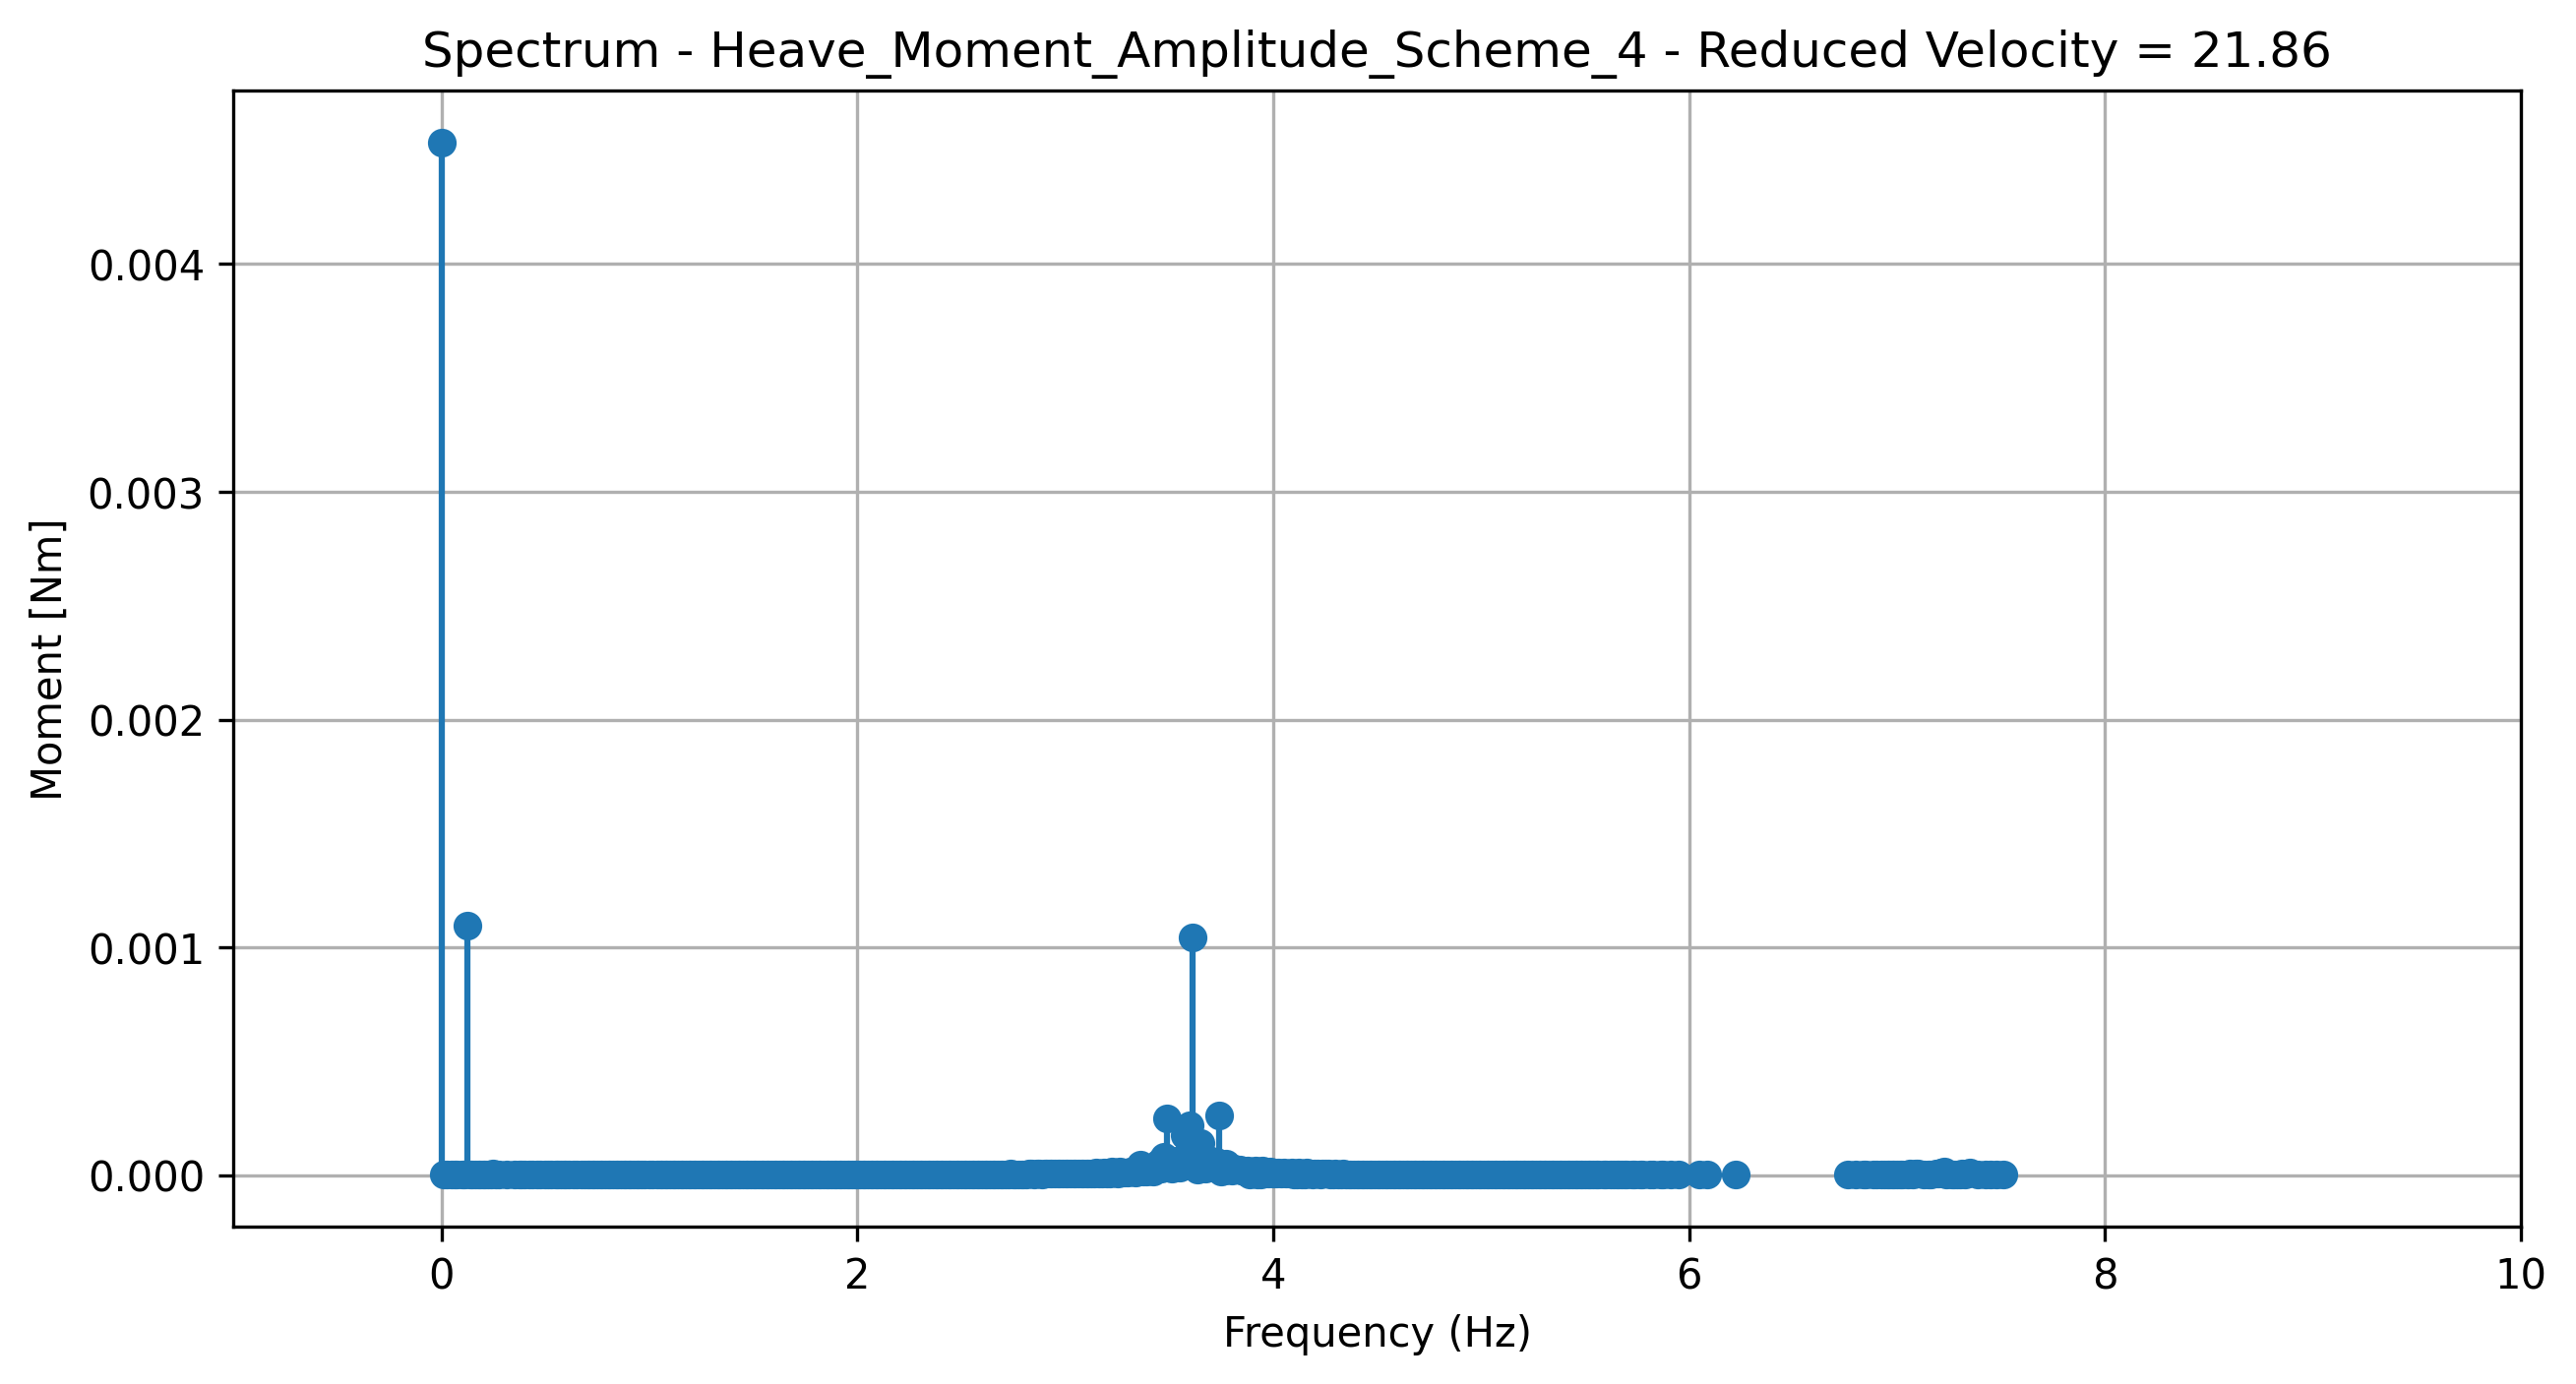
\includegraphics[width=\textwidth]{Figures/Frequency_Domain_Analysis/Heave/DFT_Moment_Amplitude_Scheme_4.png}
        \caption{}
        \label{fig:Heave_DFT_moment_amplitude_Scheme_4}
    \end{subfigure}

    % \begin{subfigure}[b]{0.45\textwidth}
    %     \centering
    %     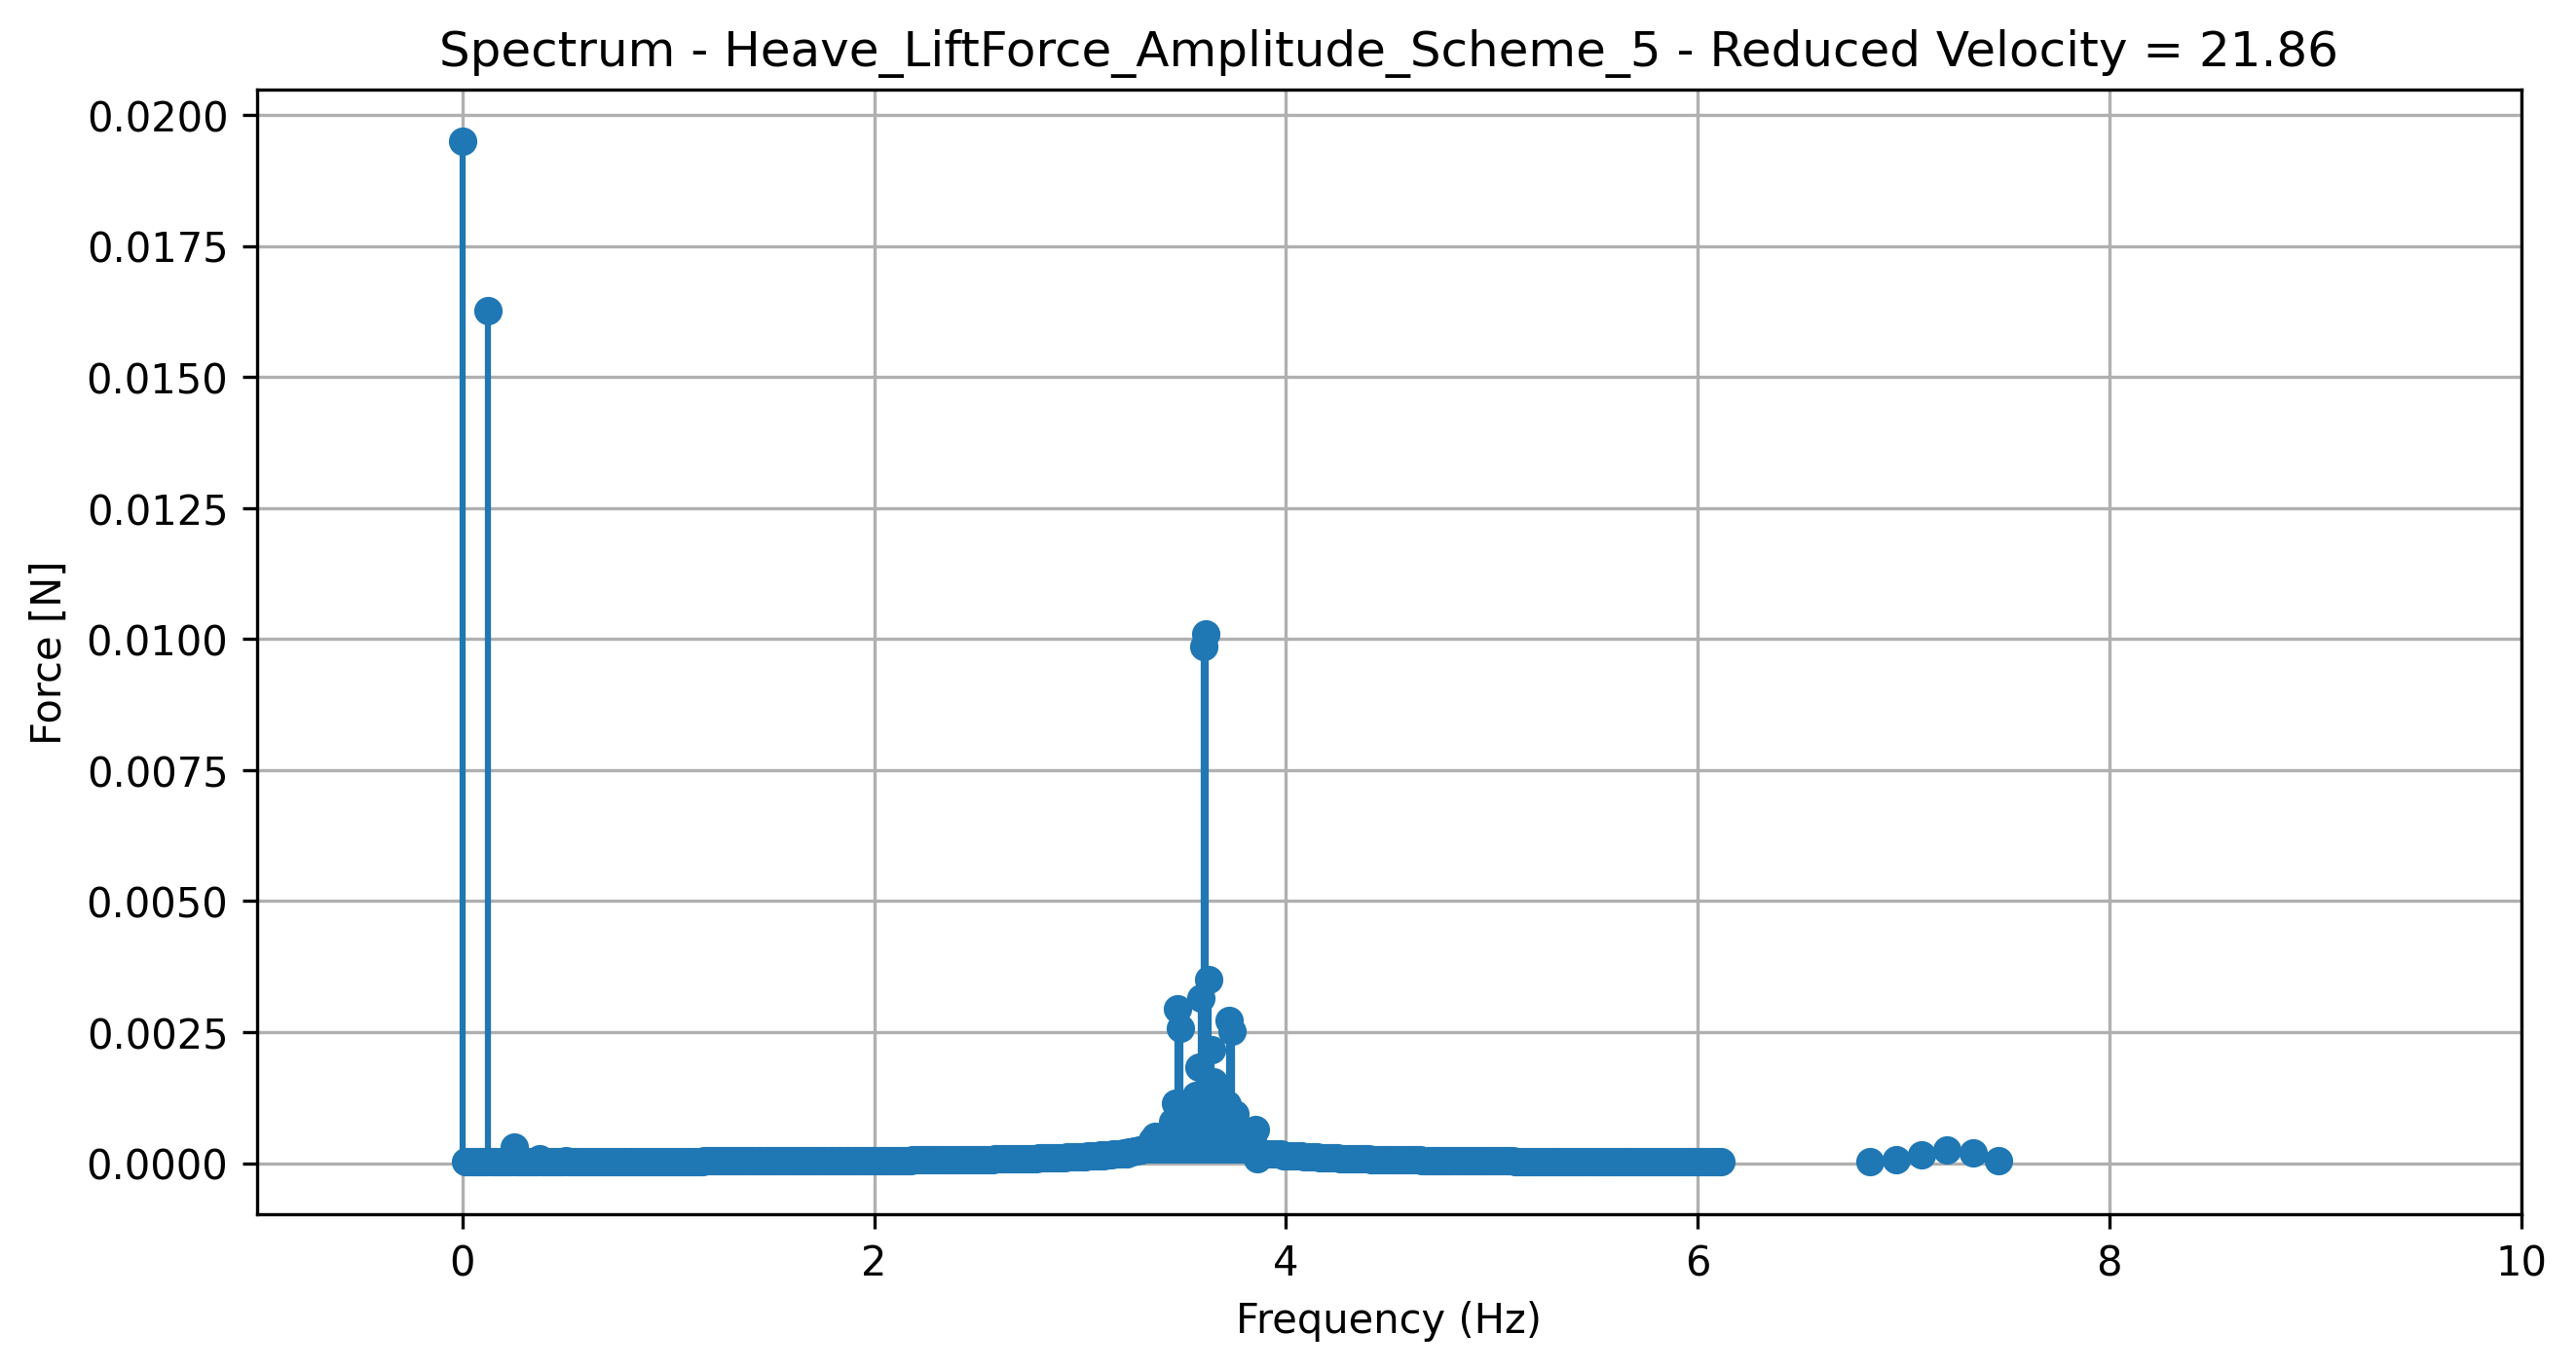
\includegraphics[width=\textwidth]{Figures/Frequency_Domain_Analysis/Heave/DFT_LiftForce_Amplitude_Scheme_5.png}
    %     \caption{}
    %     \label{fig:Heave_DFT_Fy_amplitude_Scheme_5}
    % \end{subfigure}
    % \hfill
    % \begin{subfigure}[b]{0.45\textwidth}
    %     \centering
    %     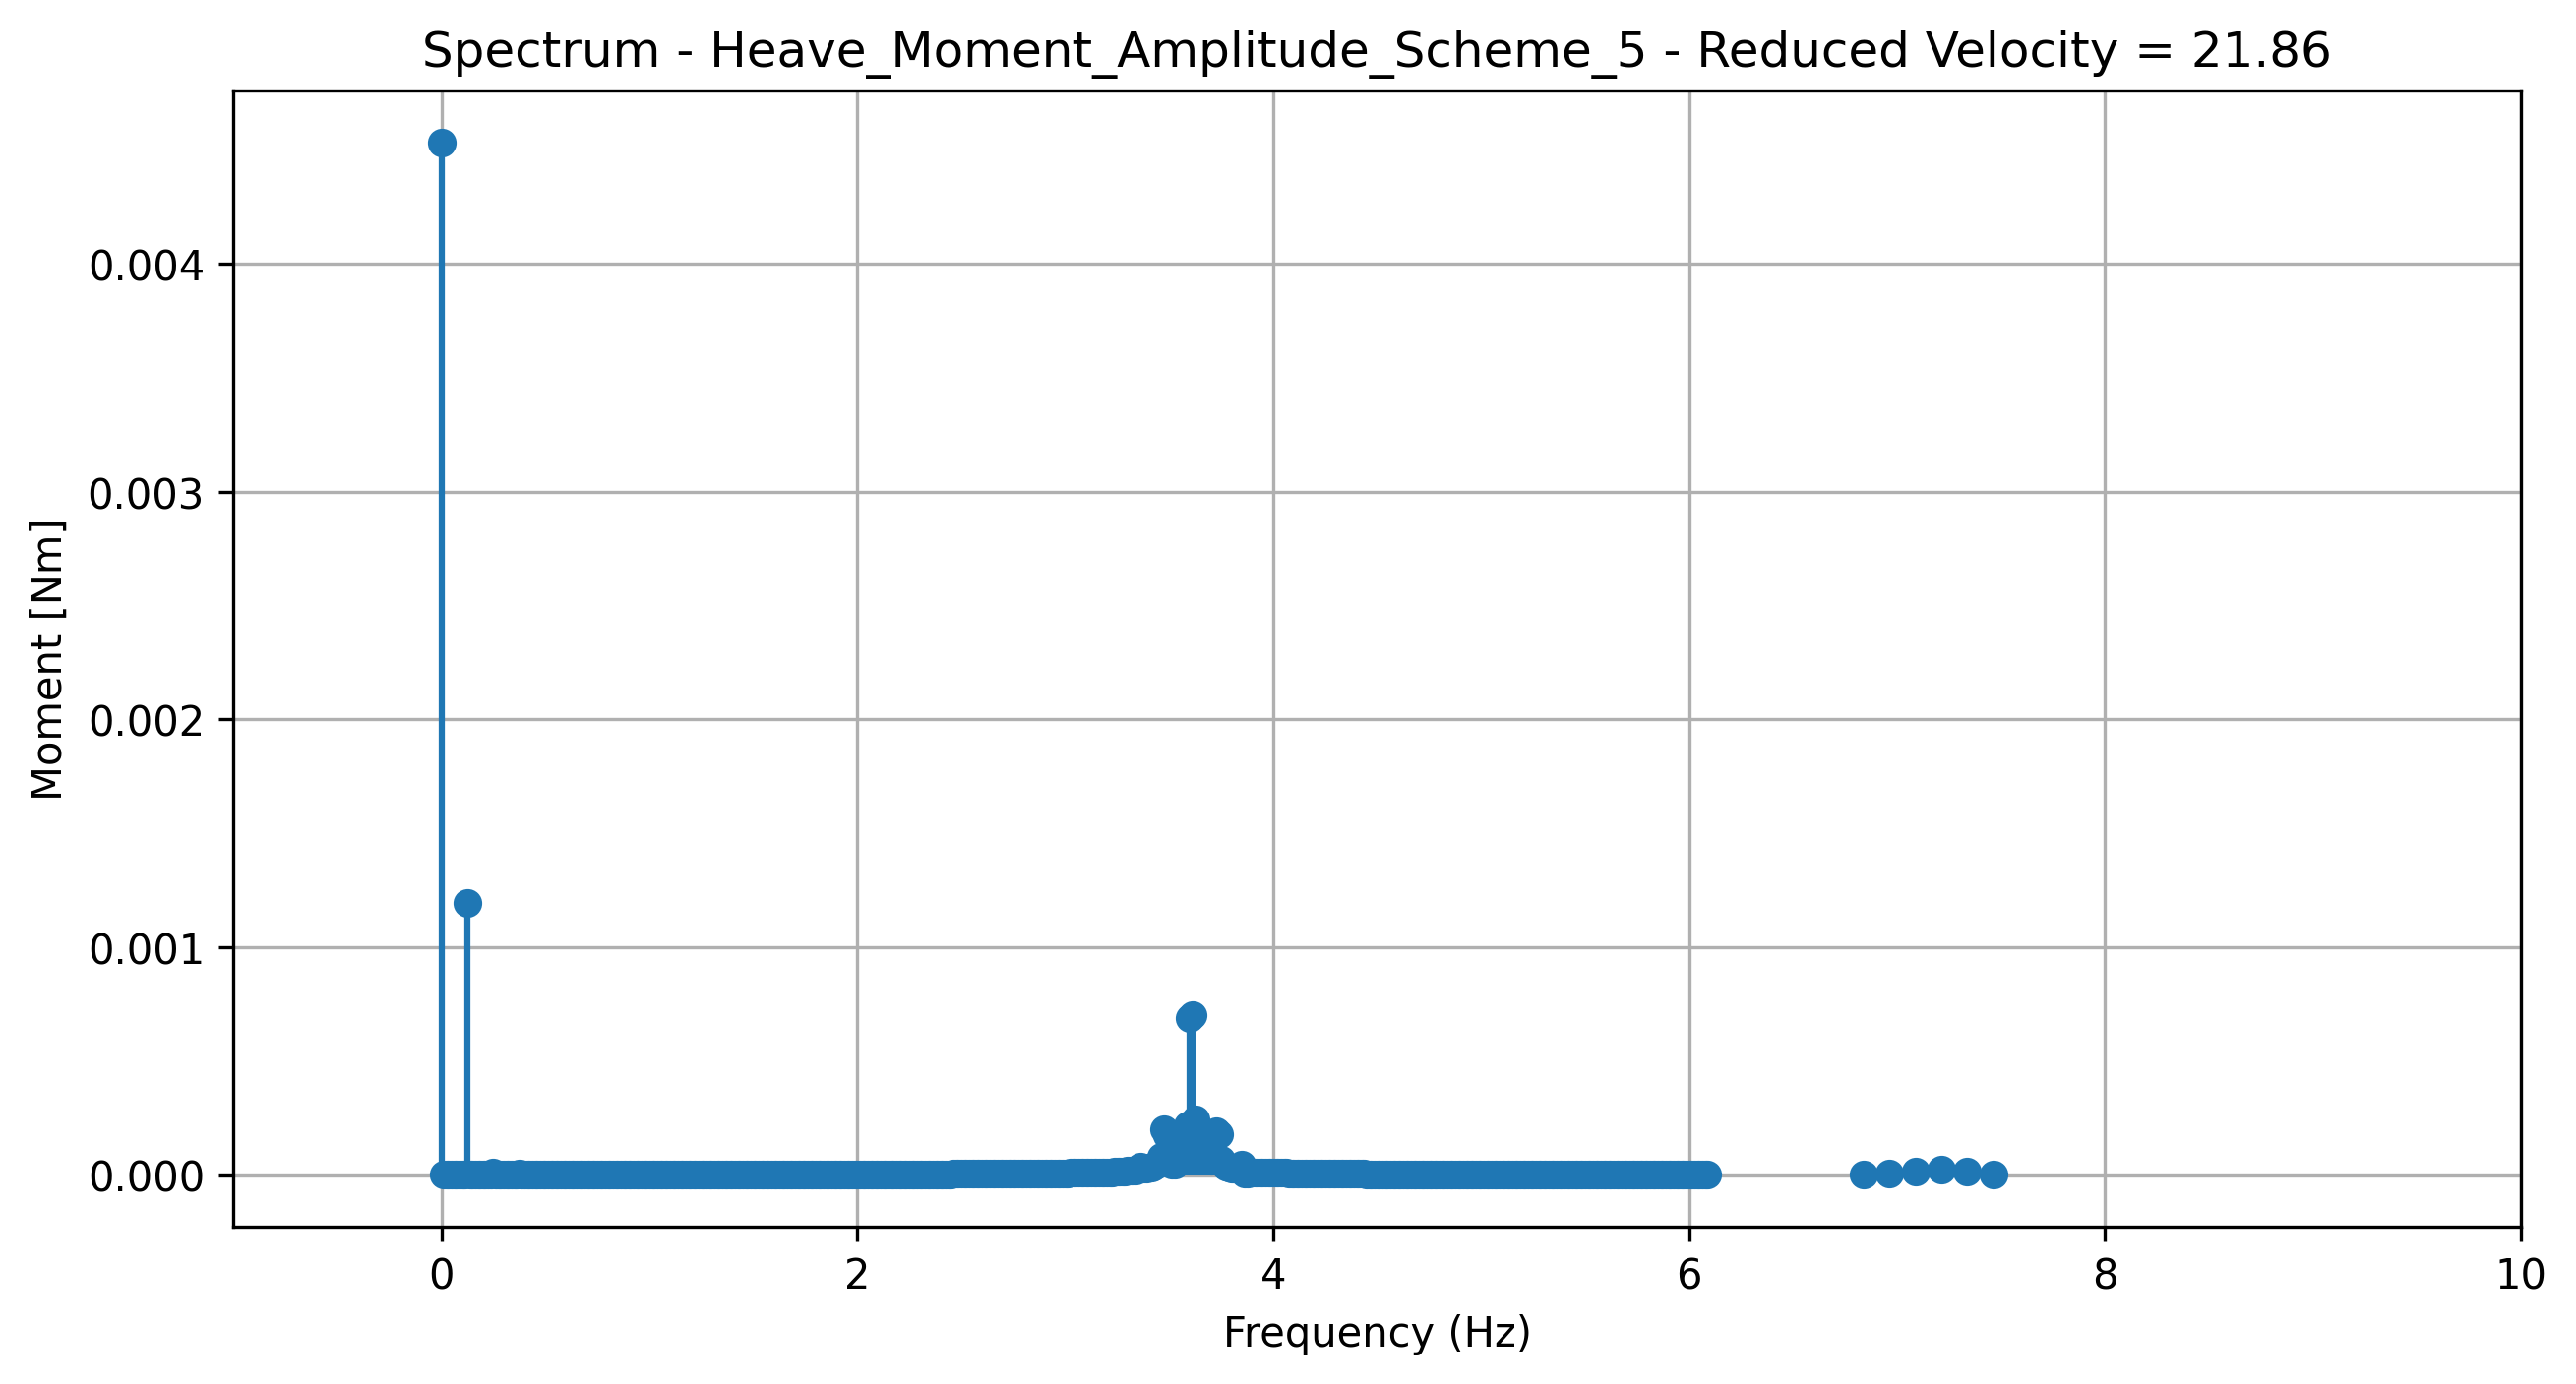
\includegraphics[width=\textwidth]{Figures/Frequency_Domain_Analysis/Heave/DFT_Moment_Amplitude_Scheme_5.png}
    %     \caption{}
    %     \label{fig:Heave_DFT_moment_amplitude_Scheme_5}
    % \end{subfigure}    

    \begin{subfigure}[b]{0.45\textwidth}
        \centering
        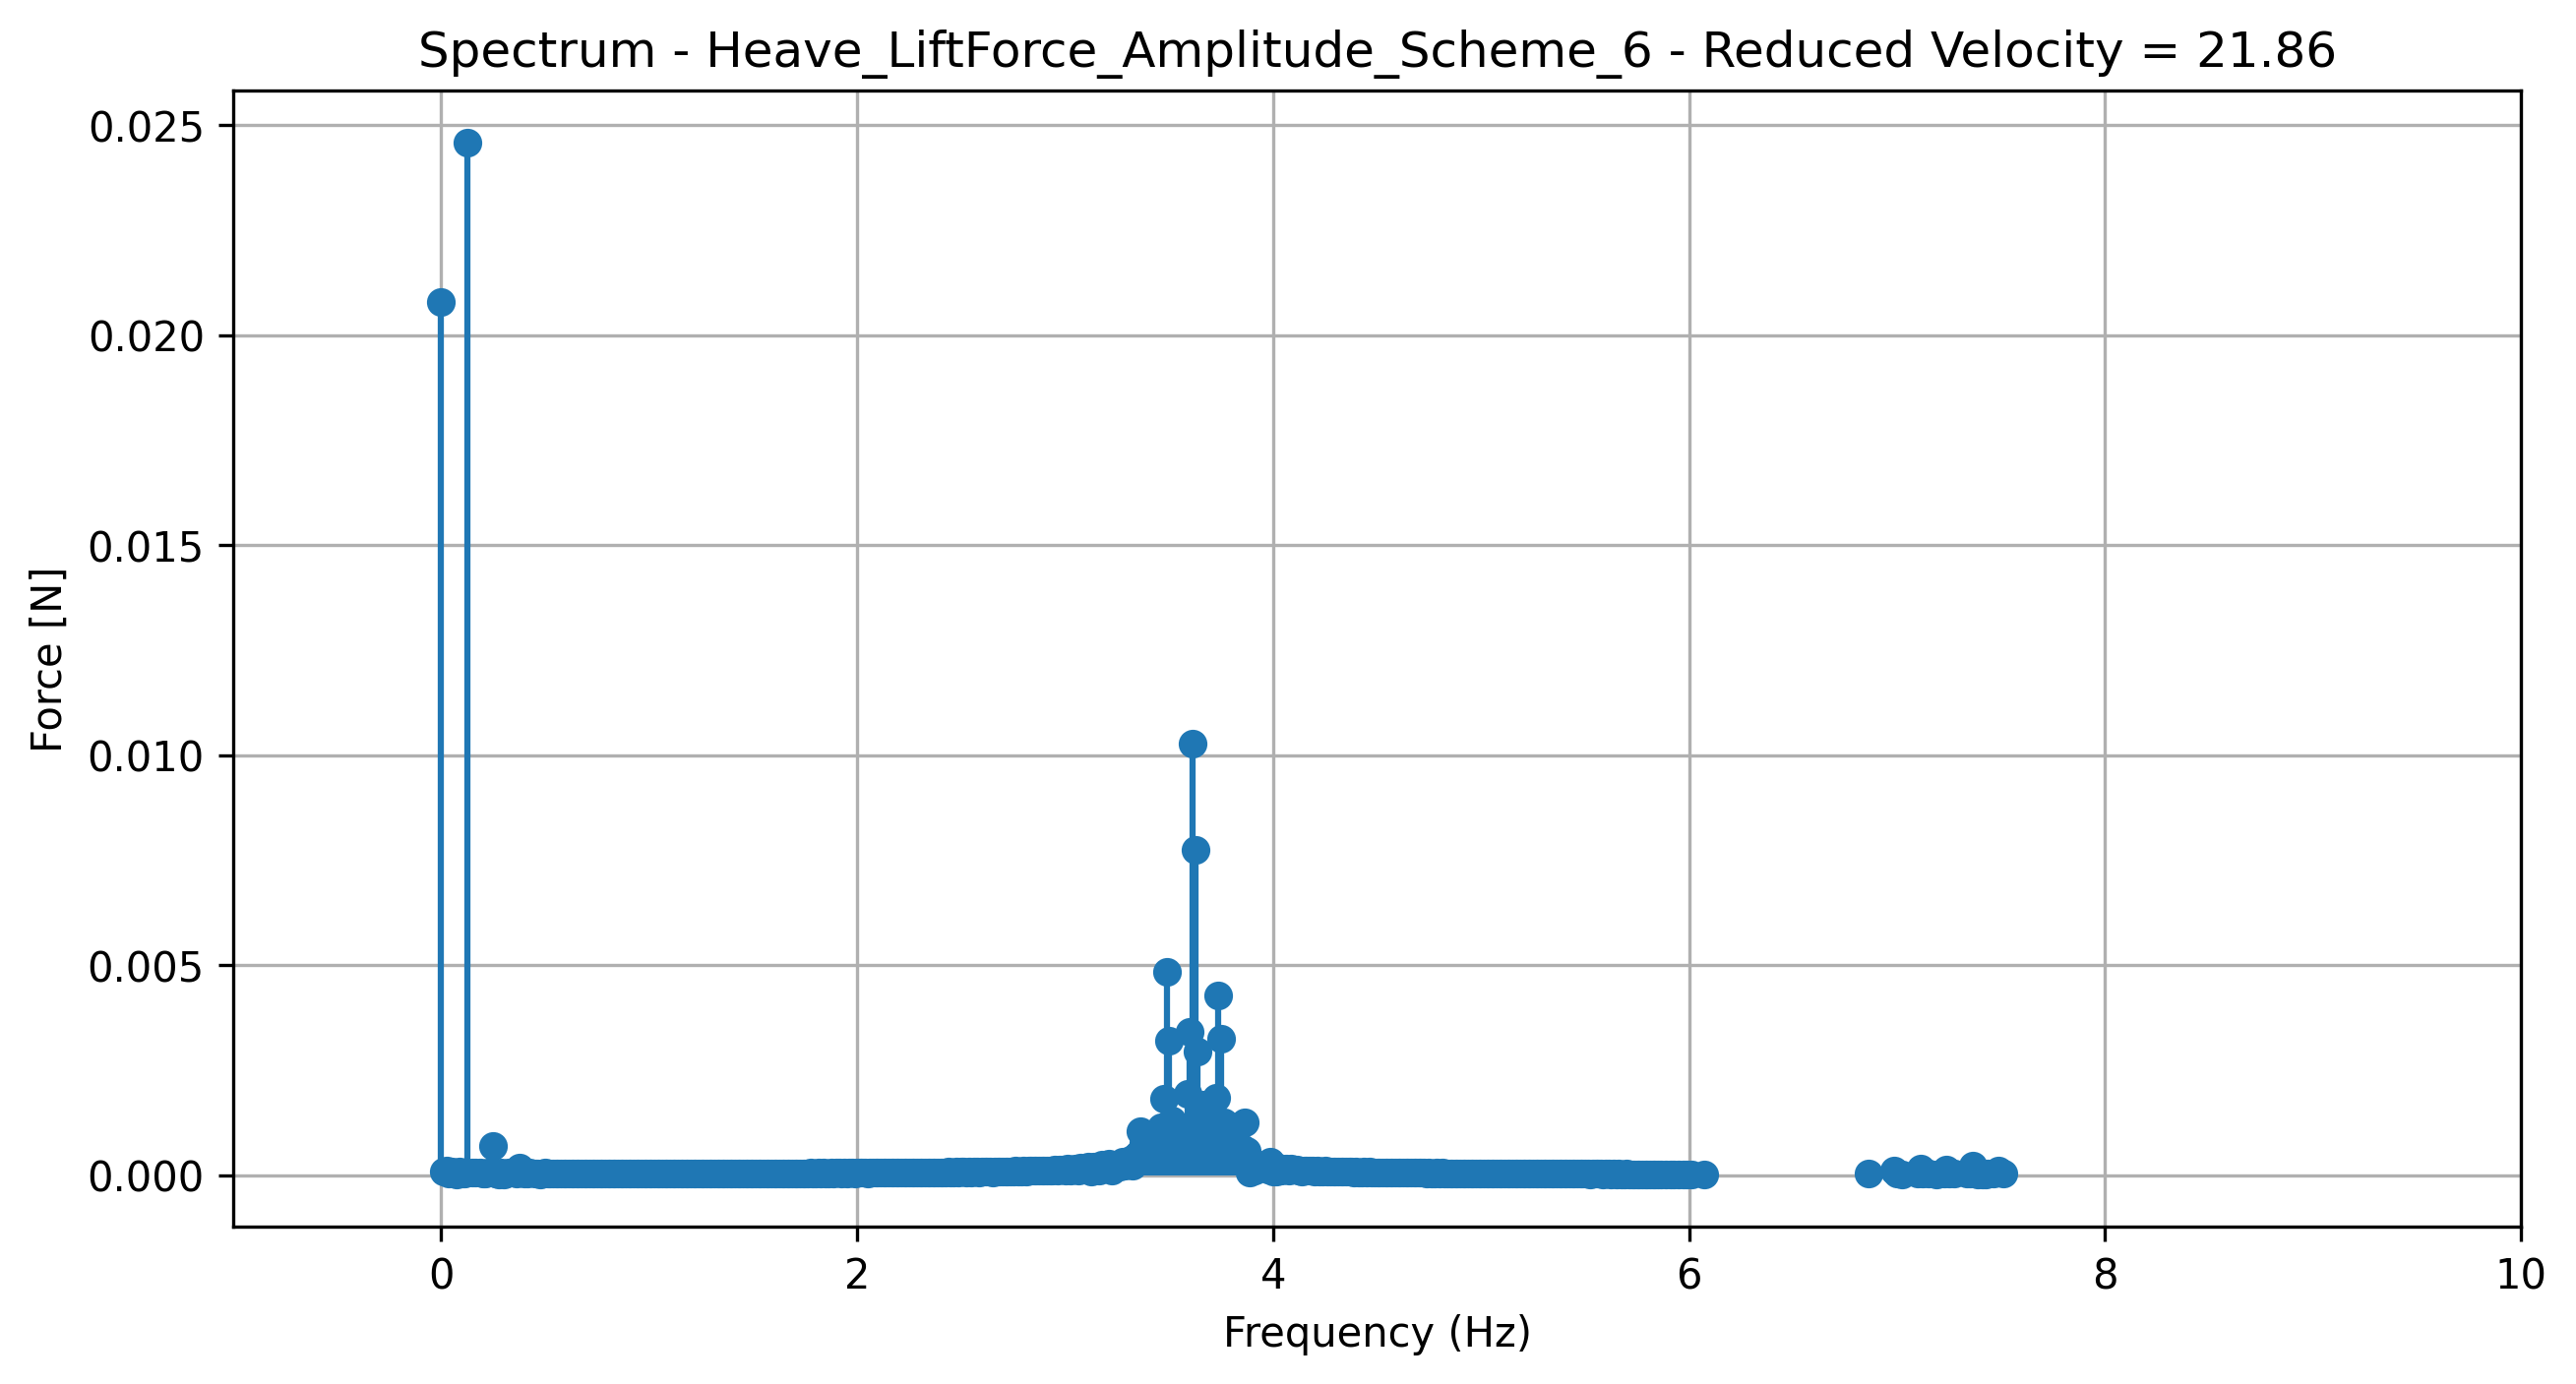
\includegraphics[width=\textwidth]{Figures/Frequency_Domain_Analysis/Heave/DFT_LiftForce_Amplitude_Scheme_6.png}
        \caption{}
        \label{fig:Heave_DFT_Fy_amplitude_Scheme_6}
    \end{subfigure}
    \hfill
    \begin{subfigure}[b]{0.45\textwidth}
        \centering
        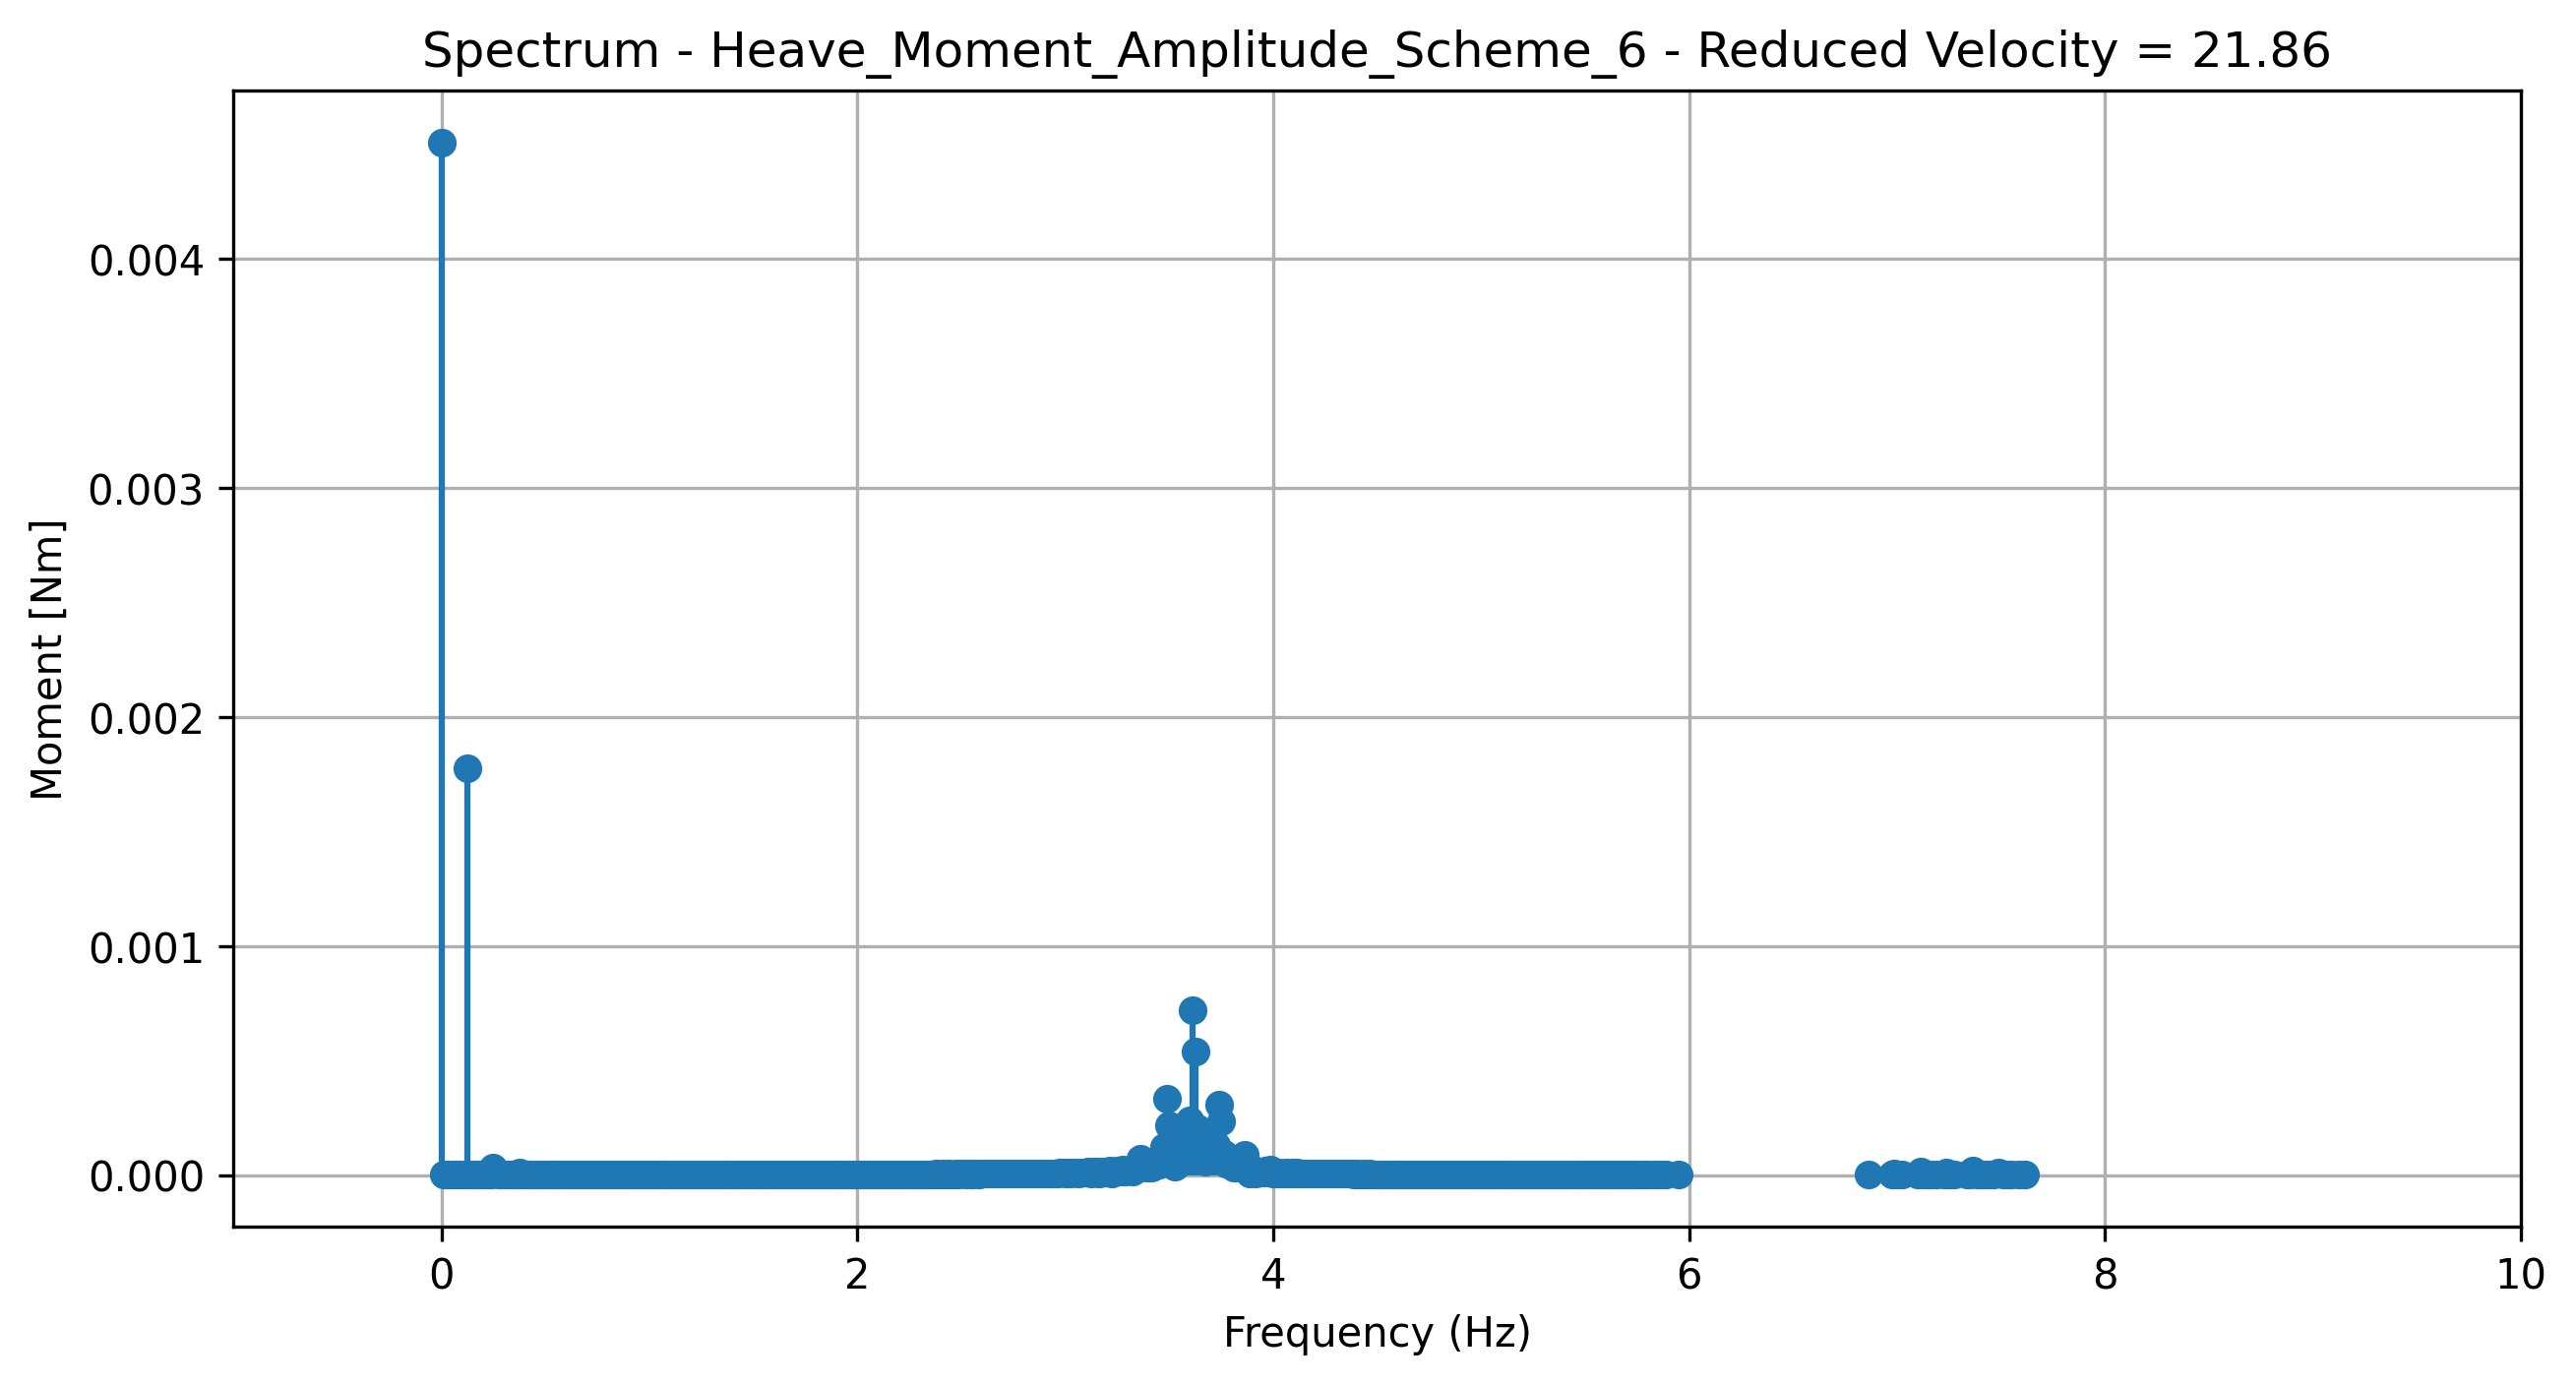
\includegraphics[width=\textwidth]{Figures/Frequency_Domain_Analysis/Heave/DFT_Moment_Amplitude_Scheme_6.png}
        \caption{}
        \label{fig:Heave_DFT_moment_amplitude_Scheme_6}
    \end{subfigure}

    \caption{Frequency Domain Analysis Heave}
    \label{fig:Frequency_Domain_Analysis_Heave}
\end{figure}

\begin{figure}[htbp]  
    \centering
    \begin{subfigure}[b]{0.45\textwidth}
        \centering
        
\includegraphics[width=\textwidth]{Figures/Frequency_Domain_Analysis/Pitch/DFT_LiftForce_Amplitude_Scheme_0.png}
        \caption{}
        \label{fig:Pitch_DFT_Fy_amplitude_Scheme_0}
    \end{subfigure}
    \hfill
    \begin{subfigure}[b]{0.45\textwidth}
        \centering
        
\includegraphics[width=\textwidth]{Figures/Frequency_Domain_Analysis/Pitch/DFT_Moment_Amplitude_Scheme_0.png}
        \caption{}
        \label{fig:Pitch_DFT_moment_amplitude_Scheme_0}
    \end{subfigure}
    
    % \begin{subfigure}[b]{0.45\textwidth}
    %     \centering
    %     
\includegraphics[width=\textwidth]{Figures/Frequency_Domain_Analysis/Pitch/DFT_LiftForce_Amplitude_Scheme_1.png}
    %     \caption{}
    %     \label{fig:Pitch_DFT_Fy_amplitude_Scheme_1}
    % \end{subfigure}
    % \hfill
    % \begin{subfigure}[b]{0.45\textwidth}
    %     \centering
    %     
\includegraphics[width=\textwidth]{Figures/Frequency_Domain_Analysis/Pitch/DFT_Moment_Amplitude_Scheme_1.png}
    %     \caption{}
    %     \label{fig:Pitch_DFT_moment_amplitude_Scheme_1}
    % \end{subfigure}
    
    \begin{subfigure}[b]{0.45\textwidth}
        \centering
        
\includegraphics[width=\textwidth]{Figures/Frequency_Domain_Analysis/Pitch/DFT_LiftForce_Amplitude_Scheme_2.png}
        \caption{}
        \label{fig:Pitch_DFT_Fy_amplitude_Scheme_2}
    \end{subfigure}
    \hfill
    \begin{subfigure}[b]{0.45\textwidth}
        \centering
        
\includegraphics[width=\textwidth]{Figures/Frequency_Domain_Analysis/Pitch/DFT_Moment_Amplitude_Scheme_2.png}
        \caption{}
        \label{fig:Pitch_DFT_moment_amplitude_Scheme_2}
    \end{subfigure}
    
    \begin{subfigure}[b]{0.45\textwidth}
        \centering
        
\includegraphics[width=\textwidth]{Figures/Frequency_Domain_Analysis/Pitch/DFT_LiftForce_Amplitude_Scheme_3.png}
        \caption{}
        \label{fig:Pitch_DFT_Fy_amplitude_Scheme_3}
    \end{subfigure}
    \hfill
    \begin{subfigure}[b]{0.45\textwidth}
        \centering
        
\includegraphics[width=\textwidth]{Figures/Frequency_Domain_Analysis/Pitch/DFT_Moment_Amplitude_Scheme_3.png}
        \caption{}
        \label{fig:Pitch_DFT_moment_amplitude_Scheme_3}
    \end{subfigure}

    \begin{subfigure}[b]{0.45\textwidth}
        \centering
        
\includegraphics[width=\textwidth]{Figures/Frequency_Domain_Analysis/Pitch/DFT_LiftForce_Amplitude_Scheme_4.png}
        \caption{}
        \label{fig:Pitch_DFT_Fy_amplitude_Scheme_4}
    \end{subfigure}
    \hfill
    \begin{subfigure}[b]{0.45\textwidth}
        \centering
        
\includegraphics[width=\textwidth]{Figures/Frequency_Domain_Analysis/Pitch/DFT_Moment_Amplitude_Scheme_4.png}
        \caption{}
        \label{fig:Pitch_DFT_moment_amplitude_Scheme_4}
    \end{subfigure}

    % \begin{subfigure}[b]{0.45\textwidth}
    %     \centering
    %     
\includegraphics[width=\textwidth]{Figures/Frequency_Domain_Analysis/Pitch/DFT_LiftForce_Amplitude_Scheme_5.png}
    %     \caption{}
    %     \label{fig:Pitch_DFT_Fy_amplitude_Scheme_5}
    % \end{subfigure}
    % \hfill
    % \begin{subfigure}[b]{0.45\textwidth}
    %     \centering
    %     
\includegraphics[width=\textwidth]{Figures/Frequency_Domain_Analysis/Pitch/DFT_Moment_Amplitude_Scheme_5.png}
    %     \caption{}
    %     \label{fig:Pitch_DFT_moment_amplitude_Scheme_5}
    % \end{subfigure}    

    \begin{subfigure}[b]{0.45\textwidth}
        \centering
        
\includegraphics[width=\textwidth]{Figures/Frequency_Domain_Analysis/Pitch/DFT_LiftForce_Amplitude_Scheme_6.png}
        \caption{}
        \label{fig:Pitch_DFT_Fy_amplitude_Scheme_6}
    \end{subfigure}
    \hfill
    \begin{subfigure}[b]{0.45\textwidth}
        \centering
        
\includegraphics[width=\textwidth]{Figures/Frequency_Domain_Analysis/Pitch/DFT_Moment_Amplitude_Scheme_6.png}
        \caption{}
        \label{fig:Pitch_DFT_moment_amplitude_Scheme_6}
    \end{subfigure}

    \caption{Frequency Domain Analysis Pitch}
    \label{fig:Frequency_Domain_Analysis_Pitch}
\end{figure}

\subsection{Aerodynamic Force and Moment Analysis}

In this section, the obtained aerodynamic forces and moments are compared against the prescribed motion 
amplitude to understand the nonlinearity characteristics of forces and moments. This is also 
conducted for phase of the aerodynamic forces and moments.\\

Figure~\ref{fig:Displacement_Vs_Force} shows plots of prescribed motion amplitude vs aerodynamic force and moment, and 
prescribed motion amplitude vs phase of aerodynamic force and moment, for both heave and pitch motion. These are plotted for 
a reduced velocity of 21.86. It can be observed that for heave motion, the lift force and moment amplitude 
exhibit linear behaviour with respect to the prescribed displacement. Furthermore, the phase of the force and 
moment is constant. For pitch motion, the lift force and moment shows linear behaviour upto to the pitch degree of 5
(the moment exhibits very little nonlinearity within this region). This is again consistent with the thumb rule of 5 degrees and 
spectral analysis and therefore validating the scanlan's linearity assumption \\

However, the phase is not constant either for the lift force or moment after 3 degrees. To have a 
comparative study of phase with flutter derivatives, first their relation is once again stated, then comparative study is shown. 
Derivatives $H_1$, $A_1$, $H_4$, and $A_4$ are associated with the heave motion aerodynamic 
lift, moment, and their phase. Derivatives $H_2$, $A_2$, $H_3$, and $A_3$ are associated with the pitch motion aerodynamic 
lift, moment, and their phase. $H_2$ and $A_2$ are associated with the phase of the pitch motion aerodynamic 
lift and moment.\\ 

On comparing Figure~\ref{fig:Displacement_Vs_Force} and Figure~\ref{fig:Combined_Flutter_Derivatives}, 
it is clear that the nonlinearity in flutter derivatives $A_2$ and $H_2$ is due to the phase change.
Further, on examining Figure~\ref{fig:Displacement_Vs_Force}-{h} the phase of the moment (related to derivative $A_2$), it changes 
from positive to negative at 3 degrees. And it can be observed in Figure~\ref{fig:Combined_Flutter_Derivatives} 
at 3 degrees derivative $A_2$ changes its sign. This confirms the sign change in $A_2$ is caused by the phase change. 

It is therefore concluded that the nonlinearity in derivatives $A_2$ and $H_2$ is not due to nonlinearity in the obtained forces, 
but due to the phase change.
This is reason the spectrum of the obtained forces is clean even when nonlinearity existed.
A similar behaviour was observed by --- and ---.\\ 

This observation points to the earlier discussion that Scanlan's linearity assumption is not equivalent to the principle of linear superposition. 
Though the obtained forces is be linear with respect to the prescribed motion, we cannot linearly superpose it the signals at these amplitudes.\\  

Since the plot shown before was only for the redcued velocity of 21.86, it is necessary to analyse the results for other reduced 
velocities before finalising the conclusion. The results for all reduced velocities are compiled in Figure~\ref{fig:Compiled_Displacement_Vs_Force}. 
The x-axis is same as before, the ampltiude case, but the y-axis is modified.\\

This y-axis represents aerodynamic force divided by the prescribed motion amplitude and normalised with respect to the first amplitude case. 
The normalisation is done because, different reduced velocities will obtain different values of aerodynamic force per unit motion amplitude.
Hence, normalisation allows for a better comparison of the nonlinearity characteristics across different reduced velocities.
For a simpler understanding, if the aerodynamic forces are linear, the plot should be a constant horizontal line at value of 1. If the phase is constant, 
the plot should similarly be a horizontal line.
Note that the $y$-axis limits are not uniform across subplots (this should be considered 
when comparing the degree of nonlinearity between the two figures). The non-uniform limits are 
kept to see the variations in nonlinearity even when the overall error is small.\\
    
It can be observed that for heave motion, lift force and moment, and their respective phases remain constant up to heave ratio of 5.46 
for reduced velocities above 1.71. 
The is equivalent to the behaviour observed earlier for the reduced velocity of 21.86
(Figure~\ref{fig:Displacement_Vs_Force}). For pitch motion, the lift force and moment exhibit slight nonlinearity, 
as seen for the reduced velocity of 21.86 (Figure~\ref{fig:Displacement_Vs_Force}).  
Another observation is that the nonlinearity in phase increases with increasing reduced velocity (decreasing frequency).
This further validates the behaviour observed in Figure~\ref{fig:Combined_Flutter_Derivatives}, 
where the nonlinearity in $A_2$ and $H_2$ is lower at lower reduced velocities.\\ 

The reduced velocities of 1.71 (frequency = 1.6 Hz) and 0.85 (frequency = 3.2 Hz) alone shows significant deviation 
in both heave and pitch motions. It is because they are affected by the vortex shedding effect. The spectral leakage 
from vortex shedding makes capturing derivatives at higher frequencies difficult.\\ 

To conclude, although Scanlan's assumption of linearity holds for the 
obtained forces, aerodynamic derivatives may still exhibit nonlinearity. And the essential note is that this 
nonlinear behaviour is not detectable with spectrum analysis. 

% Nonlinearity Study
\begin{figure}[htbp]  
    \centering
    \begin{subfigure}[b]{0.45\textwidth}
        \centering
        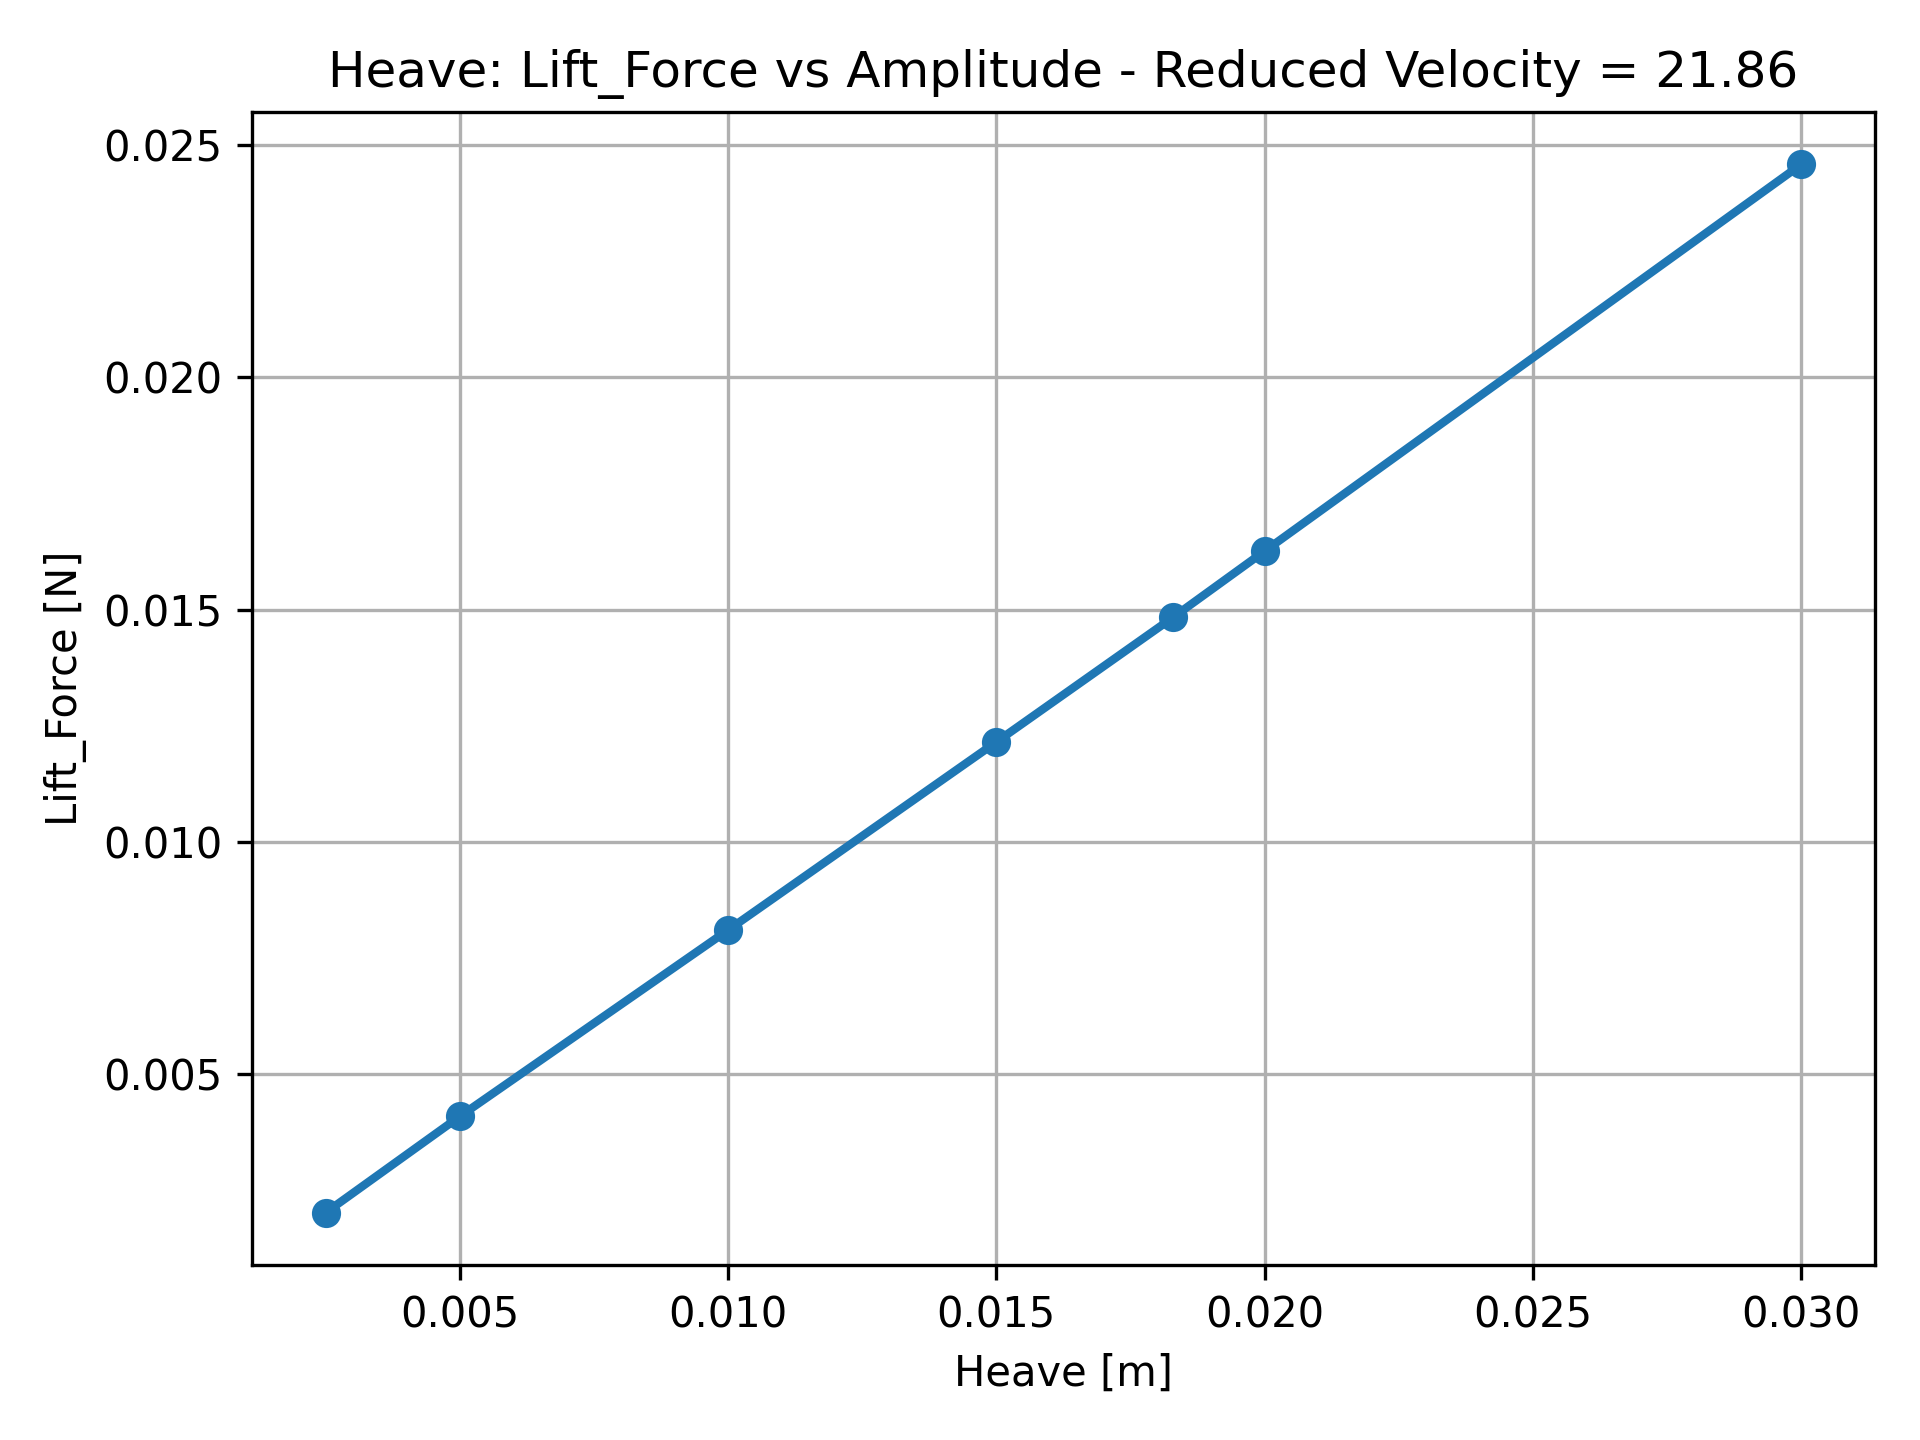
\includegraphics[width=\textwidth]{Figures/Displacement_Vs_Force/Heave/Lift_Force_vs_Amplitude.png}
        \caption{}
        \label{fig:Heave_Fy_vs_Amplitude}
    \end{subfigure}
    \hfill
    \begin{subfigure}[b]{0.45\textwidth}
        \centering
        
\includegraphics[width=\textwidth]{Figures/Displacement_Vs_Force/Pitch/Lift_Force_vs_Amplitude.png}
        \caption{}
        \label{fig:Pitch_Fy_vs_Amplitude}
    \end{subfigure}
    
    \begin{subfigure}[b]{0.45\textwidth}
        \centering
        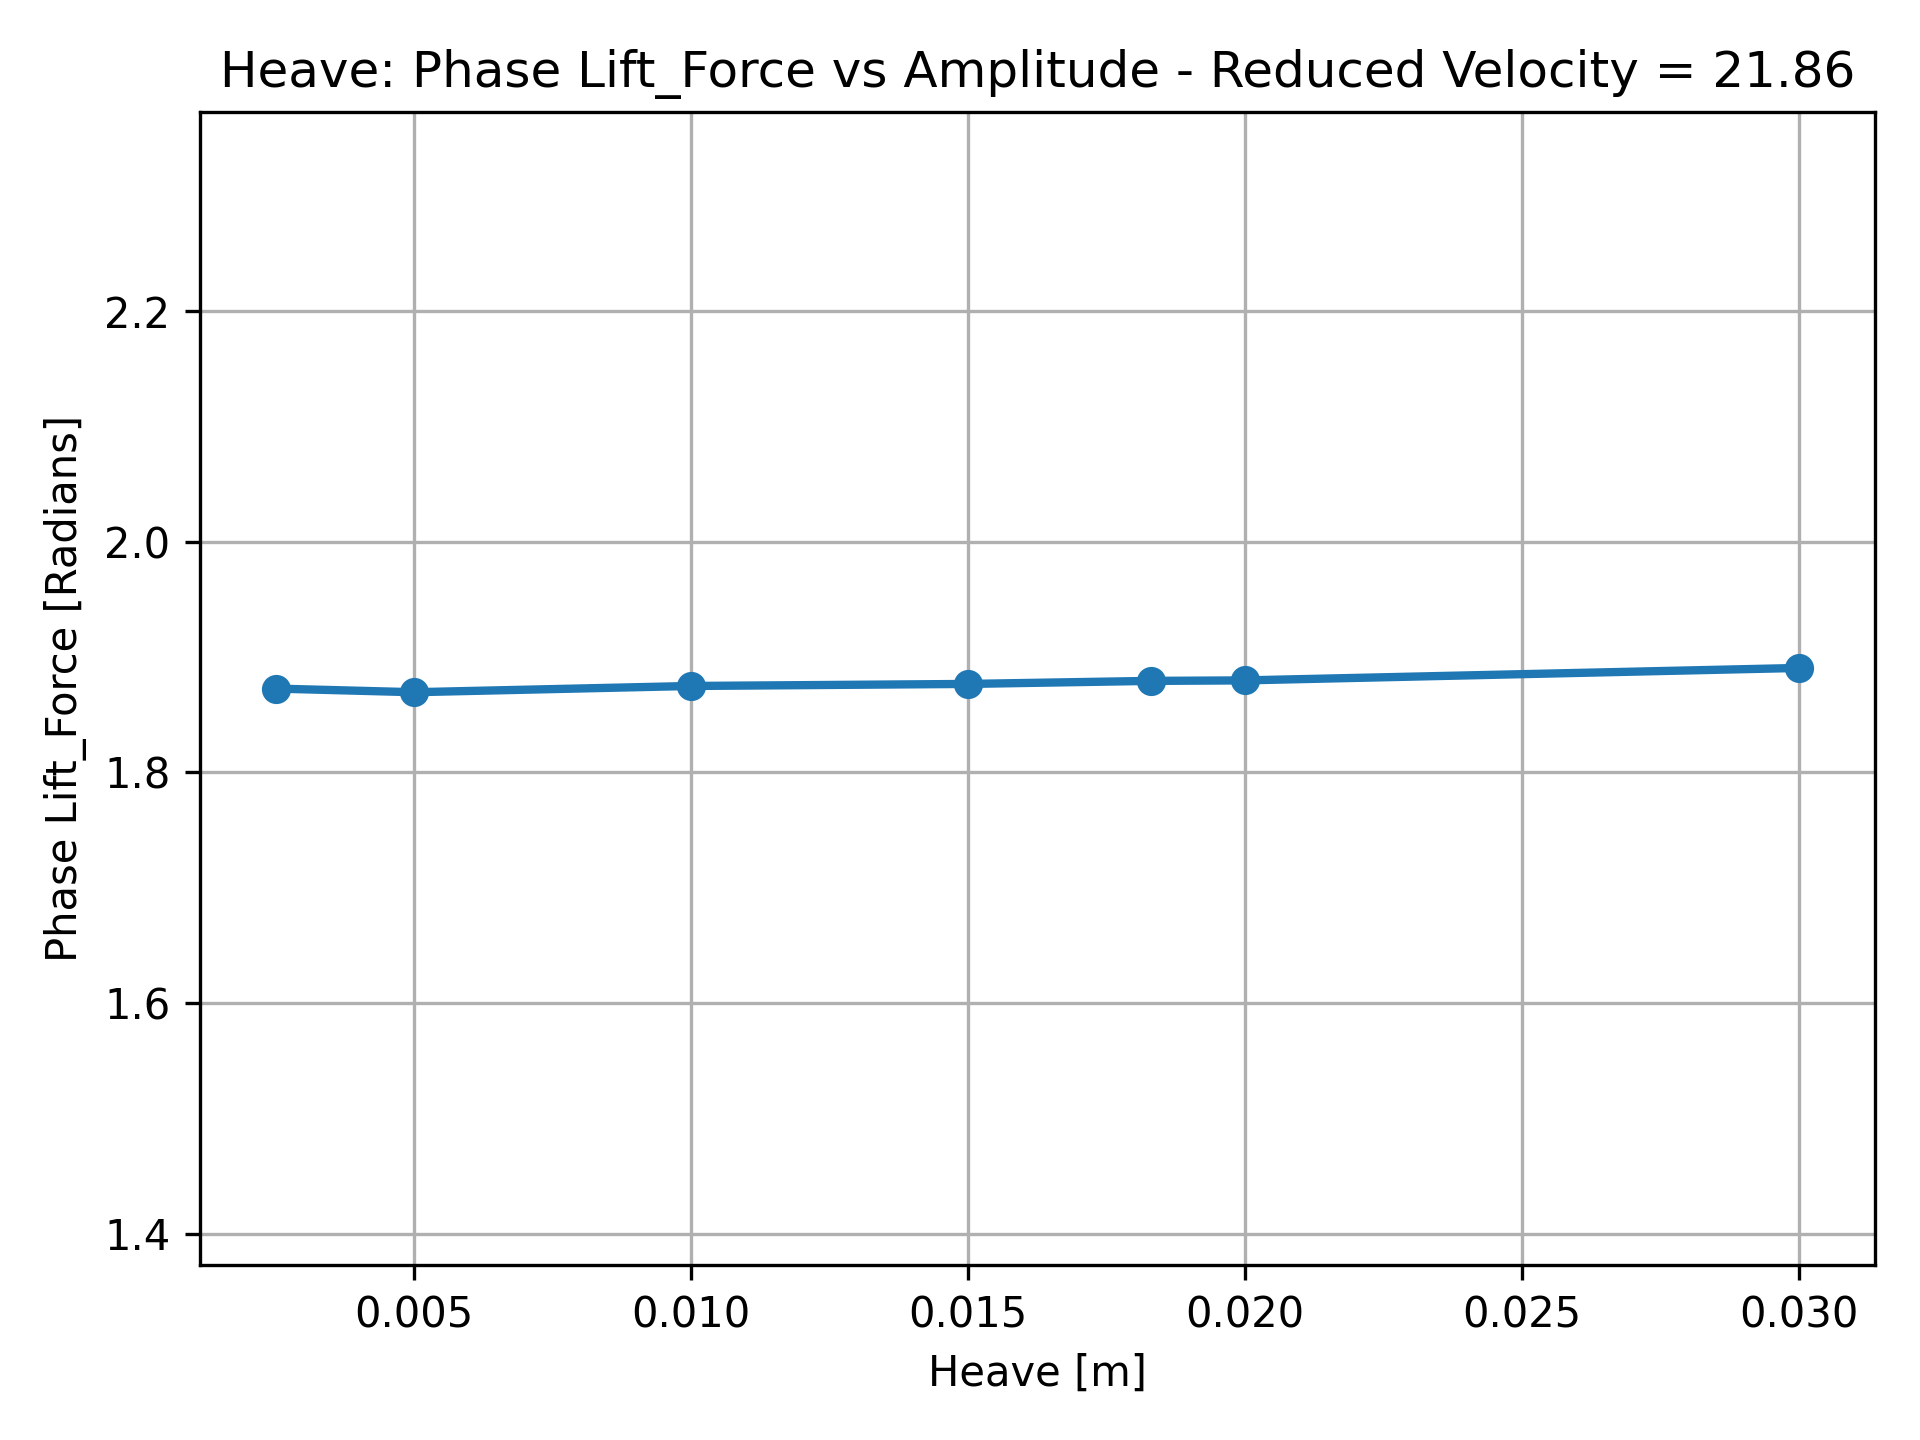
\includegraphics[width=\textwidth]{Figures/Displacement_Vs_Force/Heave/PhaseLift_Force_vs_Amplitude.png}
        \caption{}
        \label{fig:Heave_PhaseFy_vs_Amplitude}
    \end{subfigure}
    \hfill
    \begin{subfigure}[b]{0.45\textwidth}
        \centering
        
\includegraphics[width=\textwidth]{Figures/Displacement_Vs_Force/Pitch/PhaseLift_Force_vs_Amplitude.png}
        \caption{}
        \label{fig:Pitch_PhaseFy_vs_Amplitude}
    \end{subfigure}
    
    \begin{subfigure}[b]{0.45\textwidth}
        \centering
        
\includegraphics[width=\textwidth]{Figures/Displacement_Vs_Force/Heave/Moment_vs_Amplitude.png}
        \caption{}
        \label{fig:Heave_Moment_vs_Amplitude}
    \end{subfigure}
    \hfill
    \begin{subfigure}[b]{0.45\textwidth}
        \centering
        
\includegraphics[width=\textwidth]{Figures/Displacement_Vs_Force/Pitch/Moment_vs_Amplitude.png}
        \caption{}
        \label{fig:Pitch_Moment_vs_Amplitude}
    \end{subfigure}
    
    \begin{subfigure}[b]{0.45\textwidth}
        \centering
        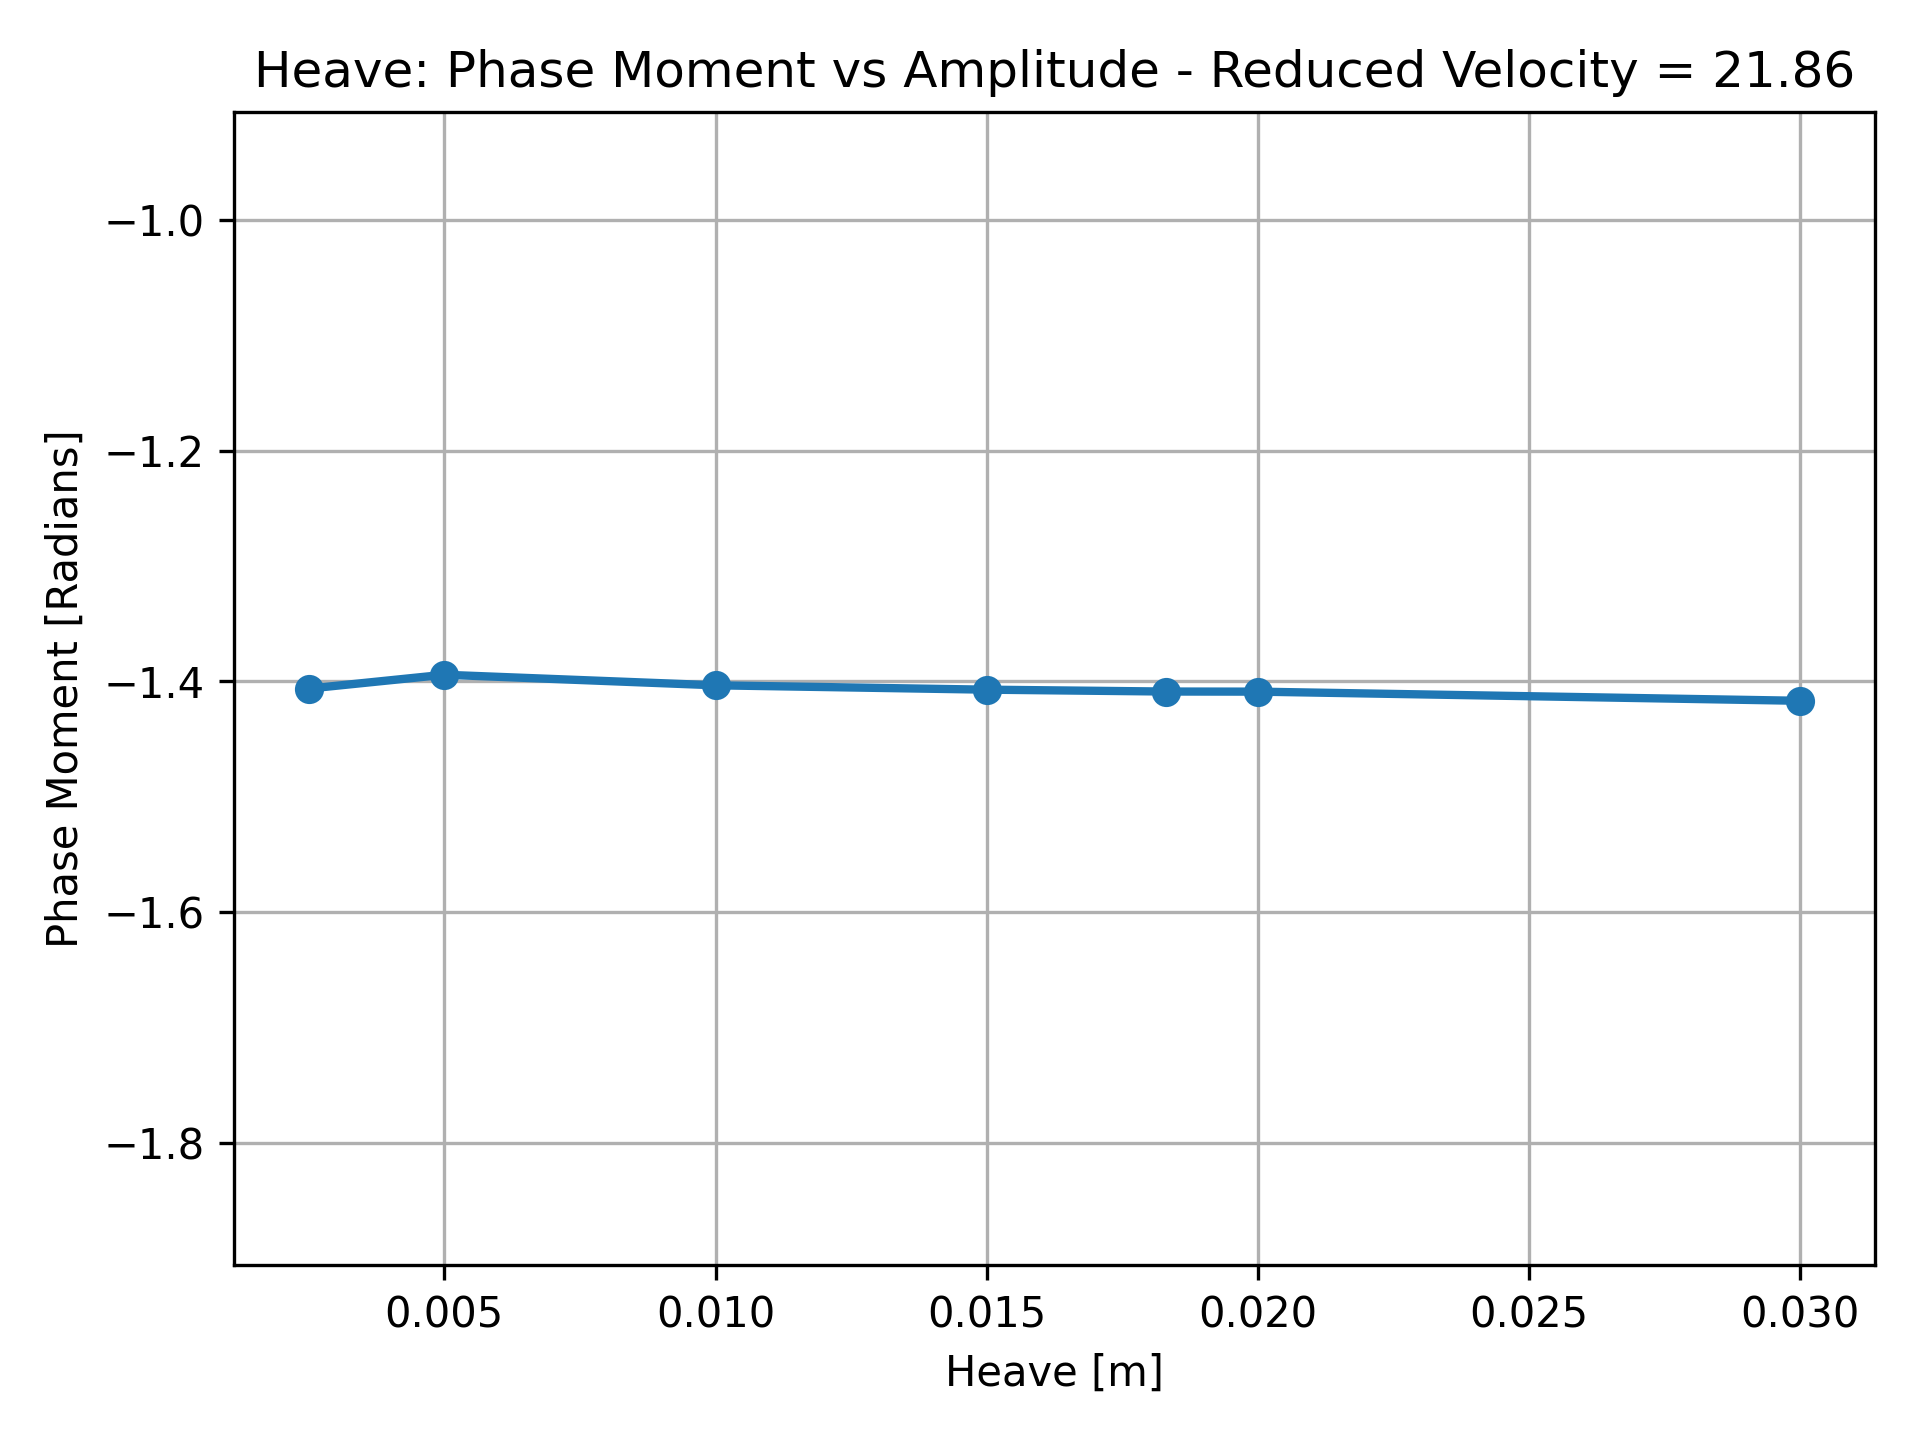
\includegraphics[width=\textwidth]{Figures/Displacement_Vs_Force/Heave/PhaseMoment_vs_Amplitude.png}
        \caption{}
        \label{fig:Heave_PhaseMx_vs_Amplitude}
    \end{subfigure}
    \hfill
    \begin{subfigure}[b]{0.45\textwidth}
        \centering
        
\includegraphics[width=\textwidth]{Figures/Displacement_Vs_Force/Pitch/PhaseMoment_vs_Amplitude.png}
        \caption{}
        \label{fig:Pitch_PhaseMx_vs_Amplitude}
    \end{subfigure}
    
    \caption{Prescribed Motion Amplitude Vs Force}
    \label{fig:Displacement_Vs_Force}
\end{figure}

% Compressed Nonlinearity Study
\begin{figure}[htbp]  
    \centering
    \begin{subfigure}[b]{0.45\textwidth}
        \centering
        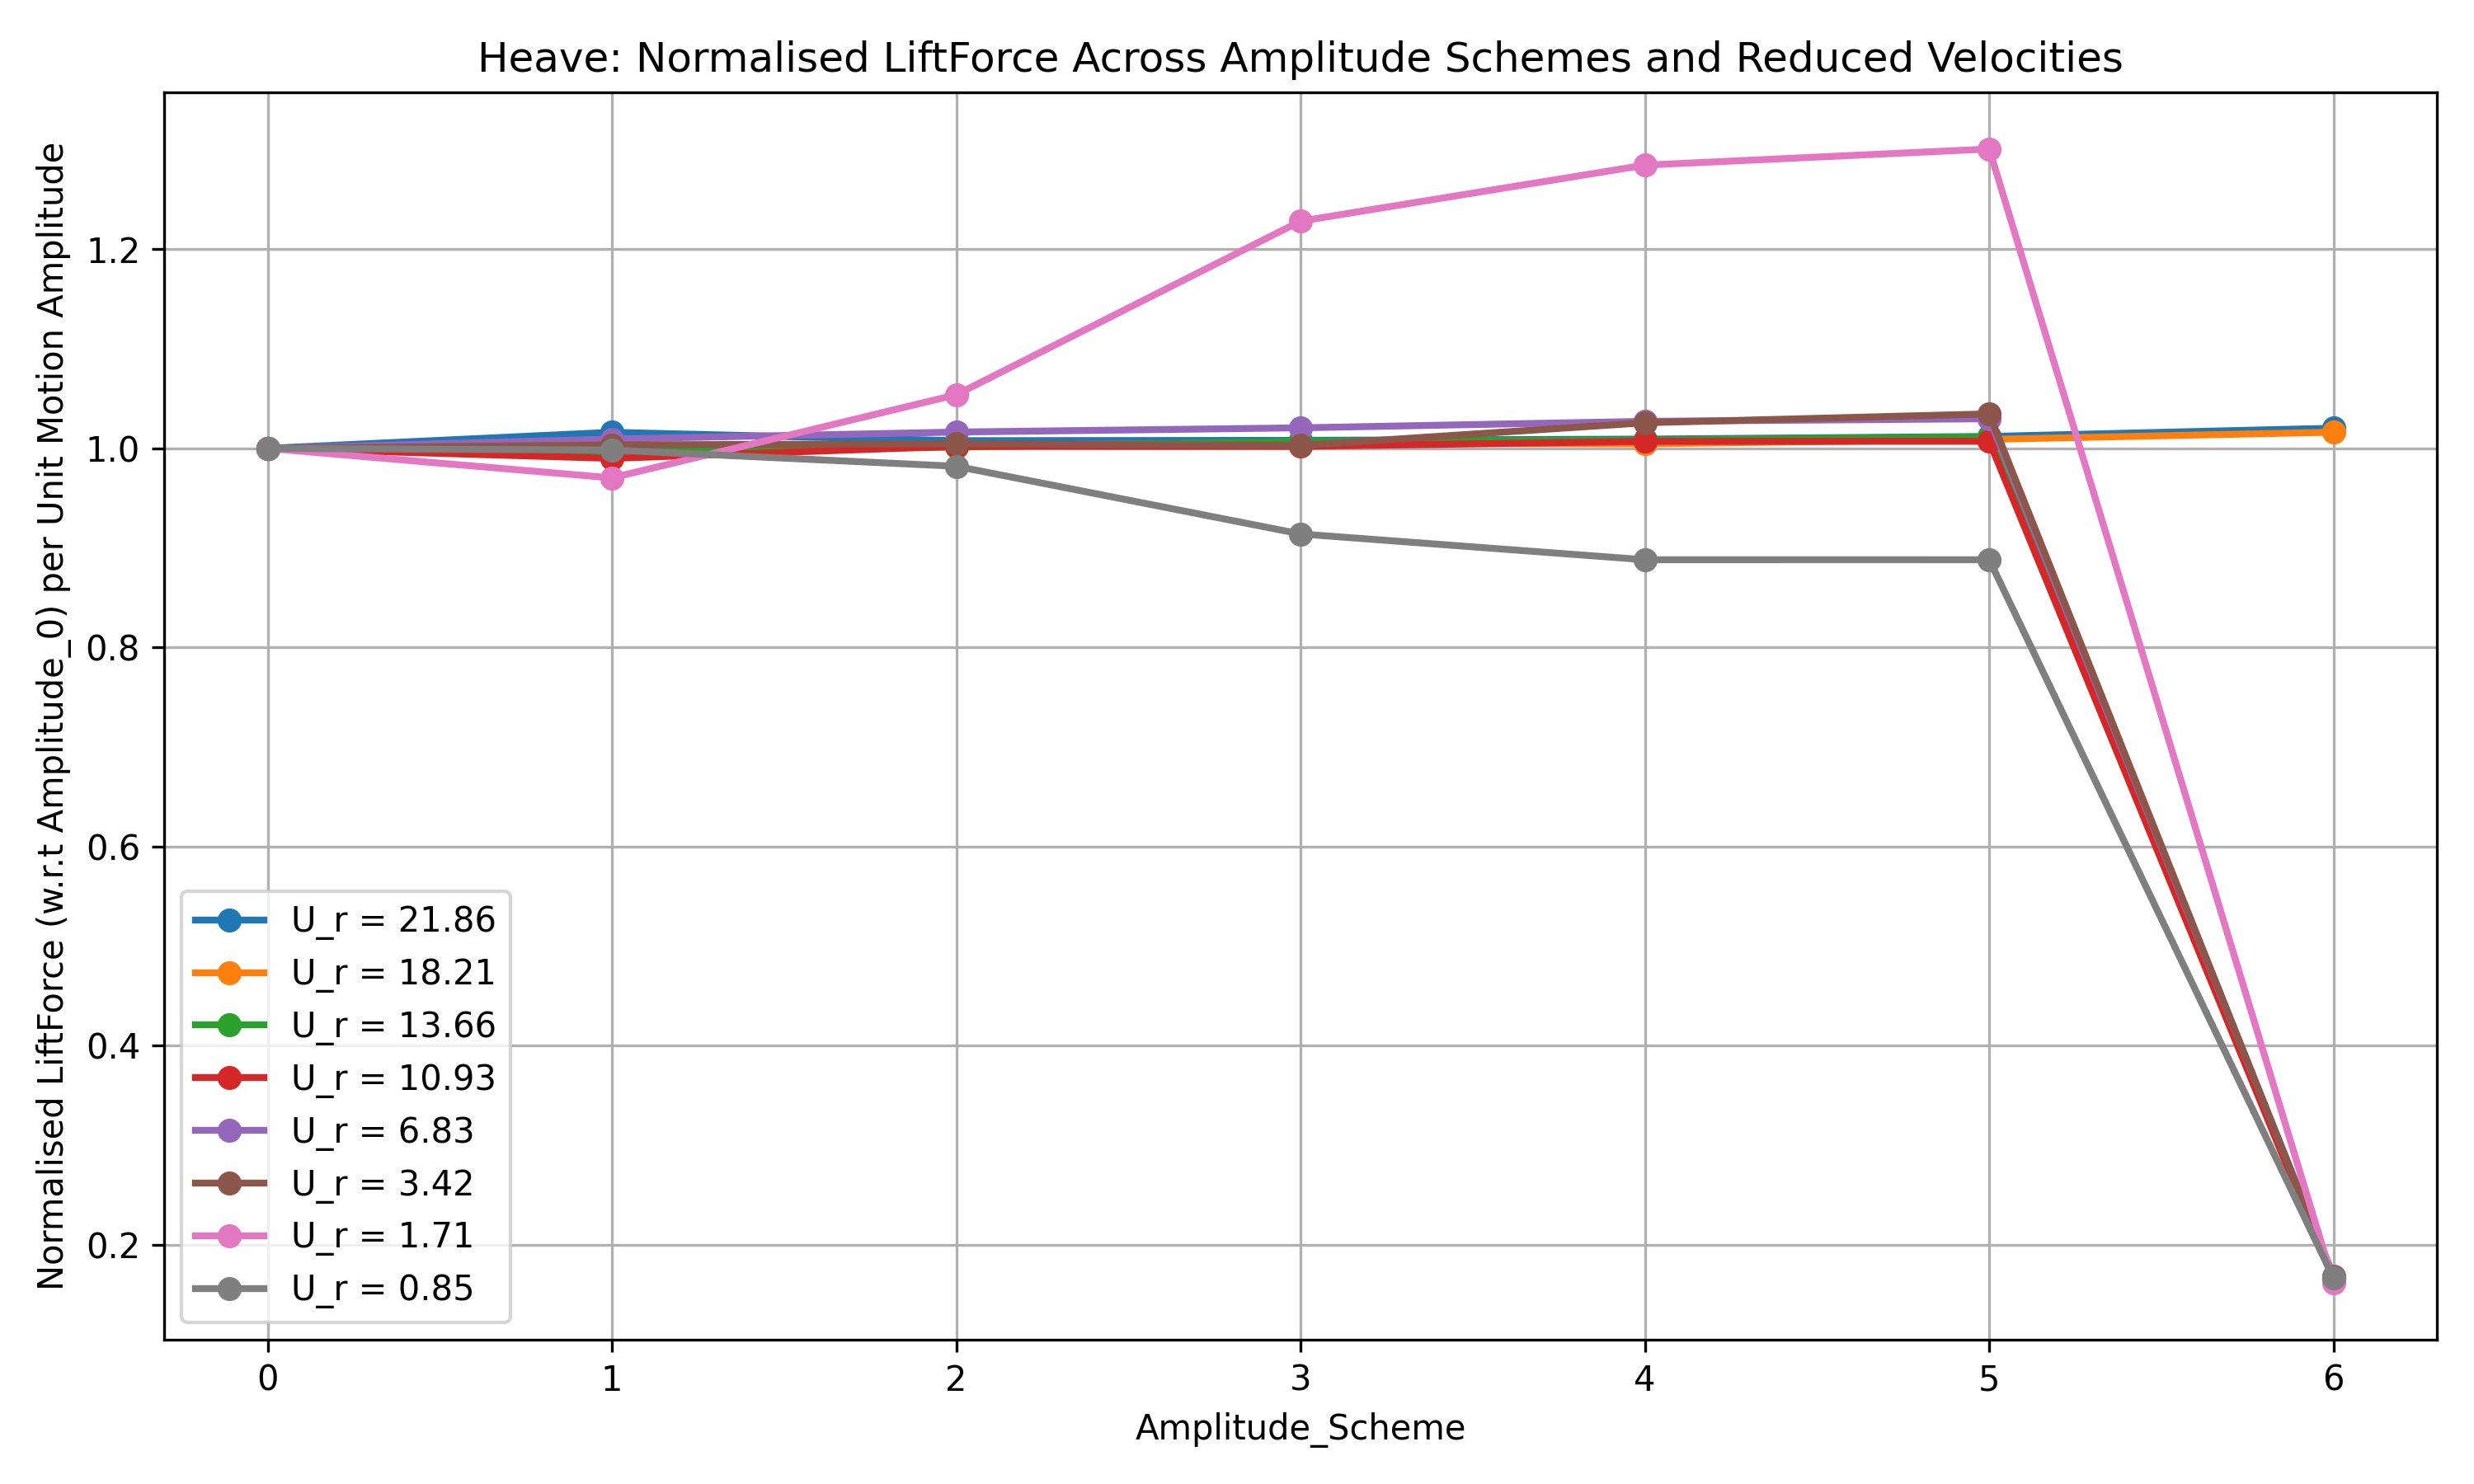
\includegraphics[width=\textwidth]{Figures/Compressed_Displacement_Vs_Force/Heave/NormalizedLift_Force_vs_Amplitude_Schemes_RelativeToFirst.png}
        \caption{}
        \label{fig:Compiled_Heave_Fy_vs_Amplitude}
    \end{subfigure}
    \hfill
    \begin{subfigure}[b]{0.45\textwidth}
        \centering
        
\includegraphics[width=\textwidth]{Figures/Compressed_Displacement_Vs_Force/Pitch/NormalizedLift_Force_vs_Amplitude_Schemes_RelativeToFirst.png}
        \caption{}
        \label{fig:Compiled_Pitch_Fy_vs_Amplitude}
    \end{subfigure}
    
    \begin{subfigure}[b]{0.45\textwidth}
        \centering
        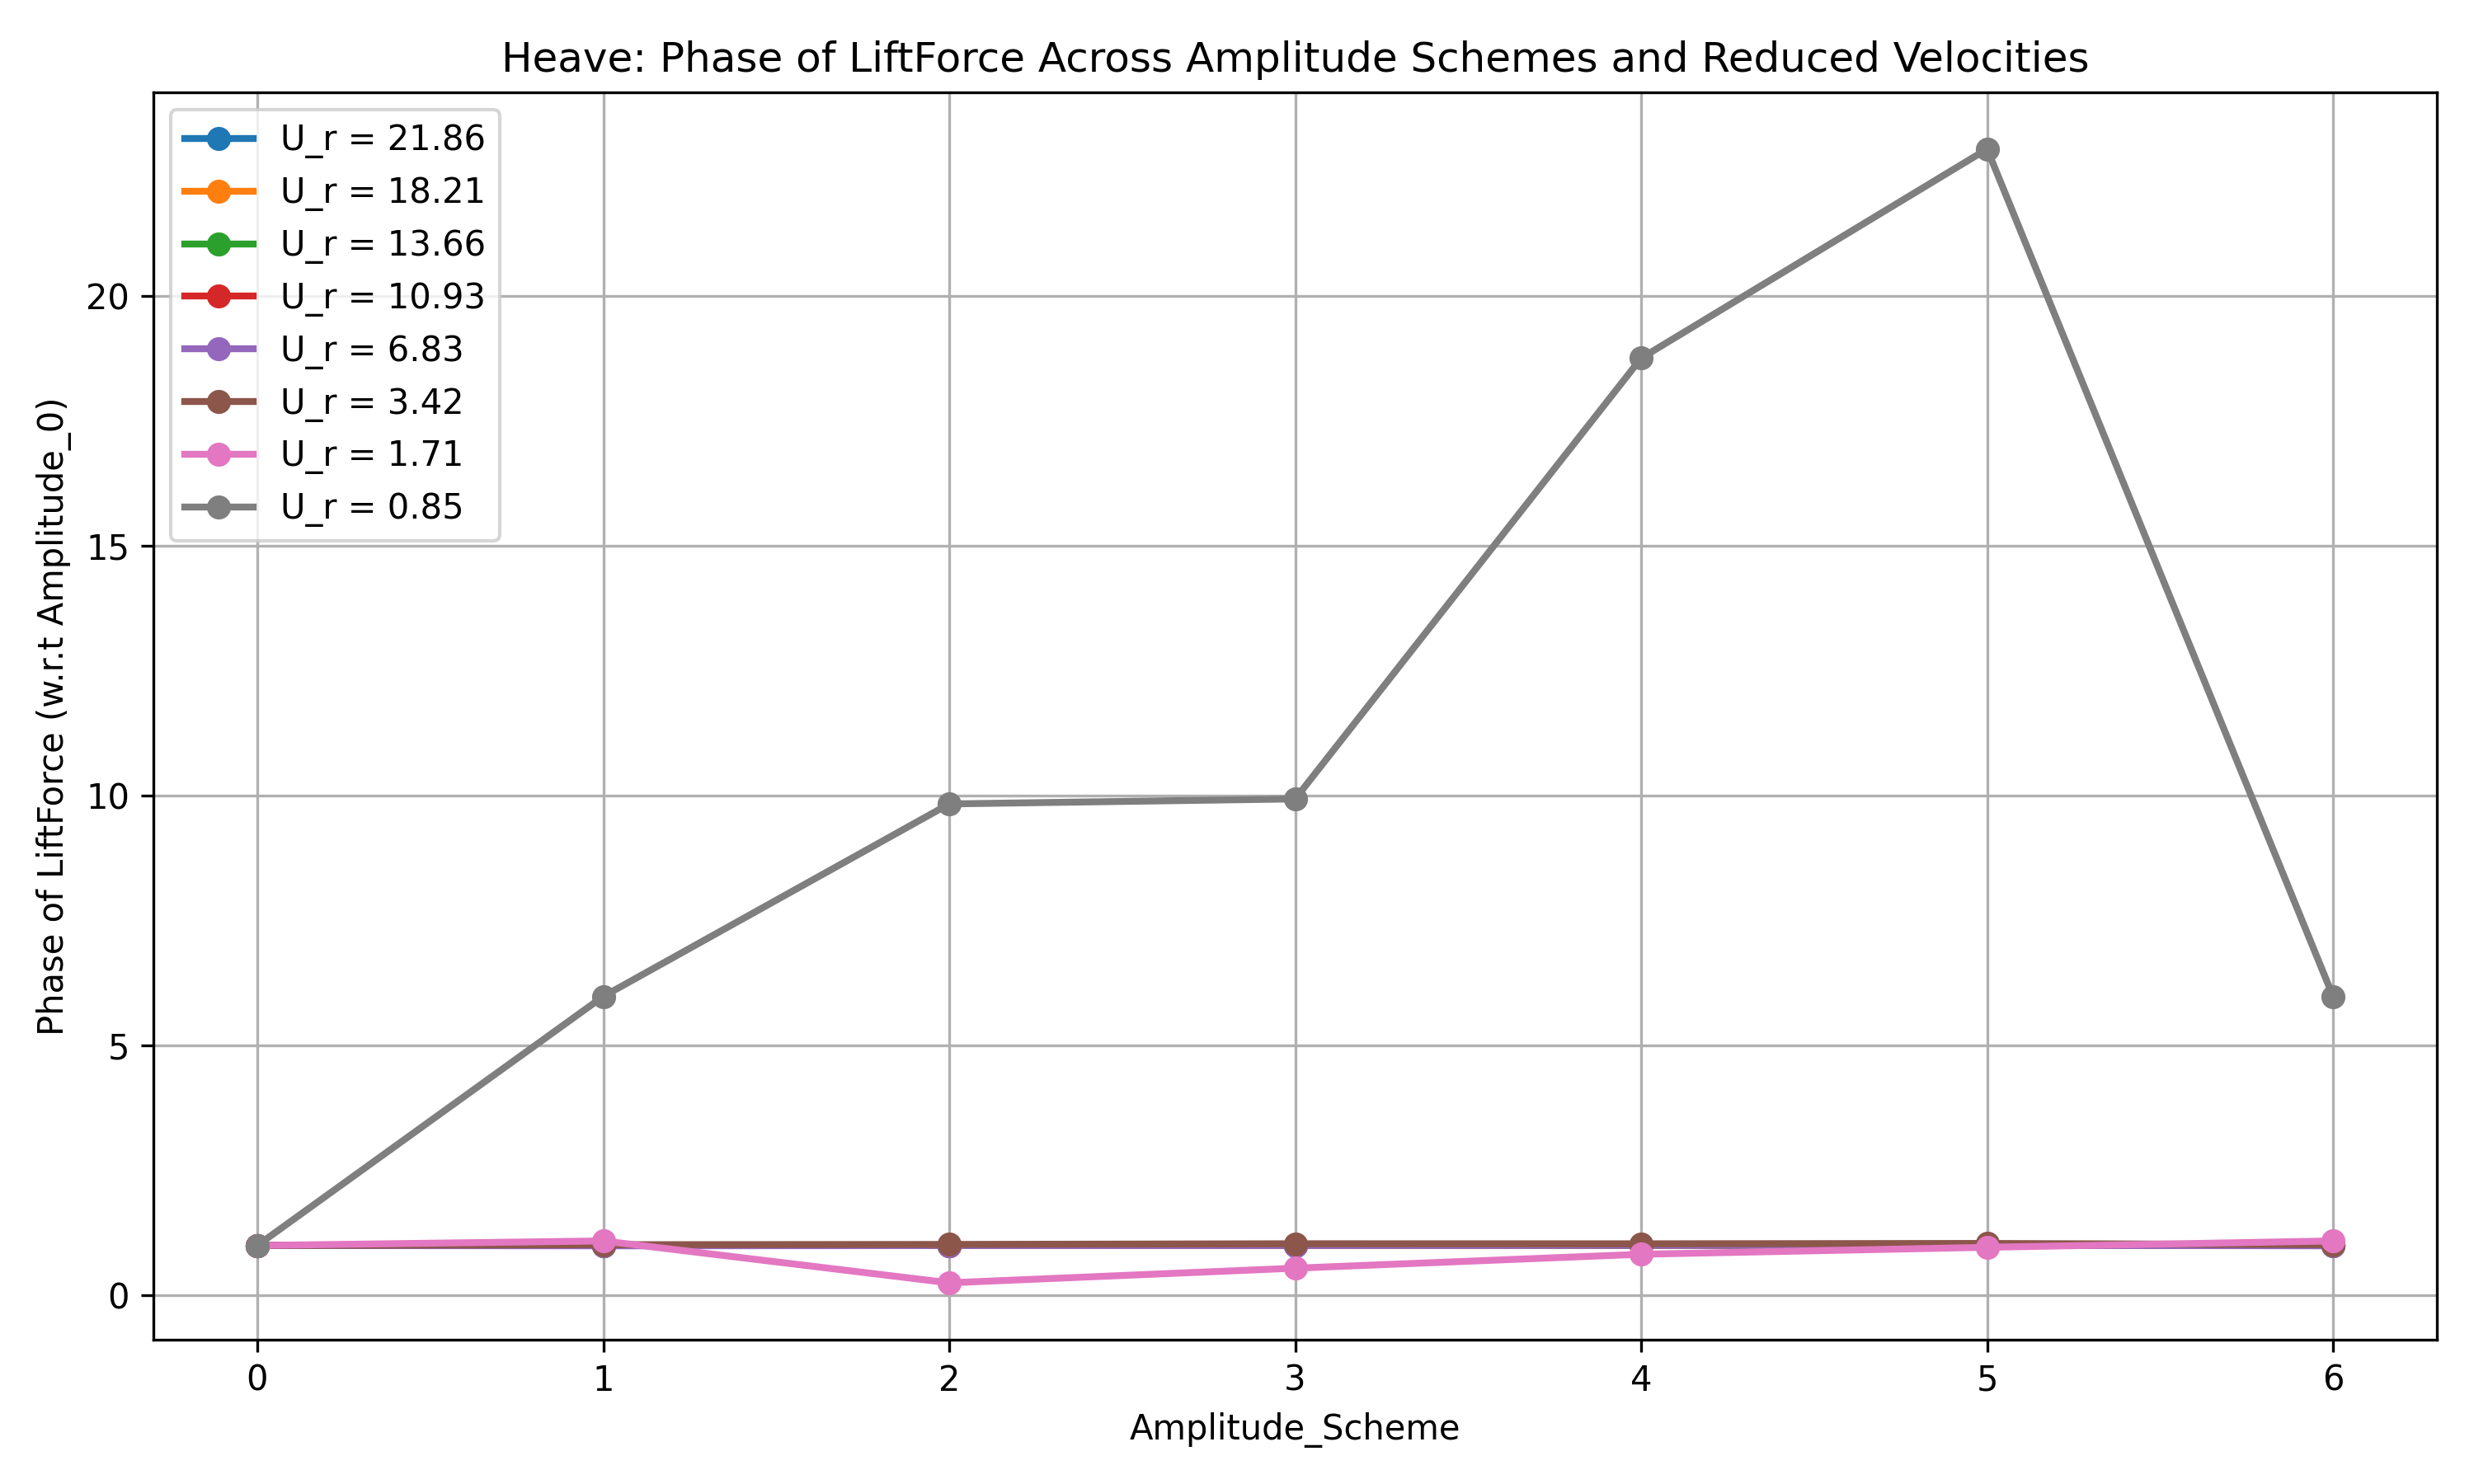
\includegraphics[width=\textwidth]{Figures/Compressed_Displacement_Vs_Force/Heave/PhaseLift_Force_vs_Amplitude_Schemes_RelativeToFirst.png}
        \caption{}
        \label{fig:Compiled_Heave_PhaseFy_vs_Amplitude}
    \end{subfigure}
    \hfill
    \begin{subfigure}[b]{0.45\textwidth}
        \centering
        
\includegraphics[width=\textwidth]{Figures/Compressed_Displacement_Vs_Force/Pitch/PhaseLift_Force_vs_Amplitude_Schemes_RelativeToFirst.png}
        \caption{}
        \label{fig:Compiled_Pitch_PhaseFy_vs_Amplitude}
    \end{subfigure}
    
    \begin{subfigure}[b]{0.45\textwidth}
        \centering
        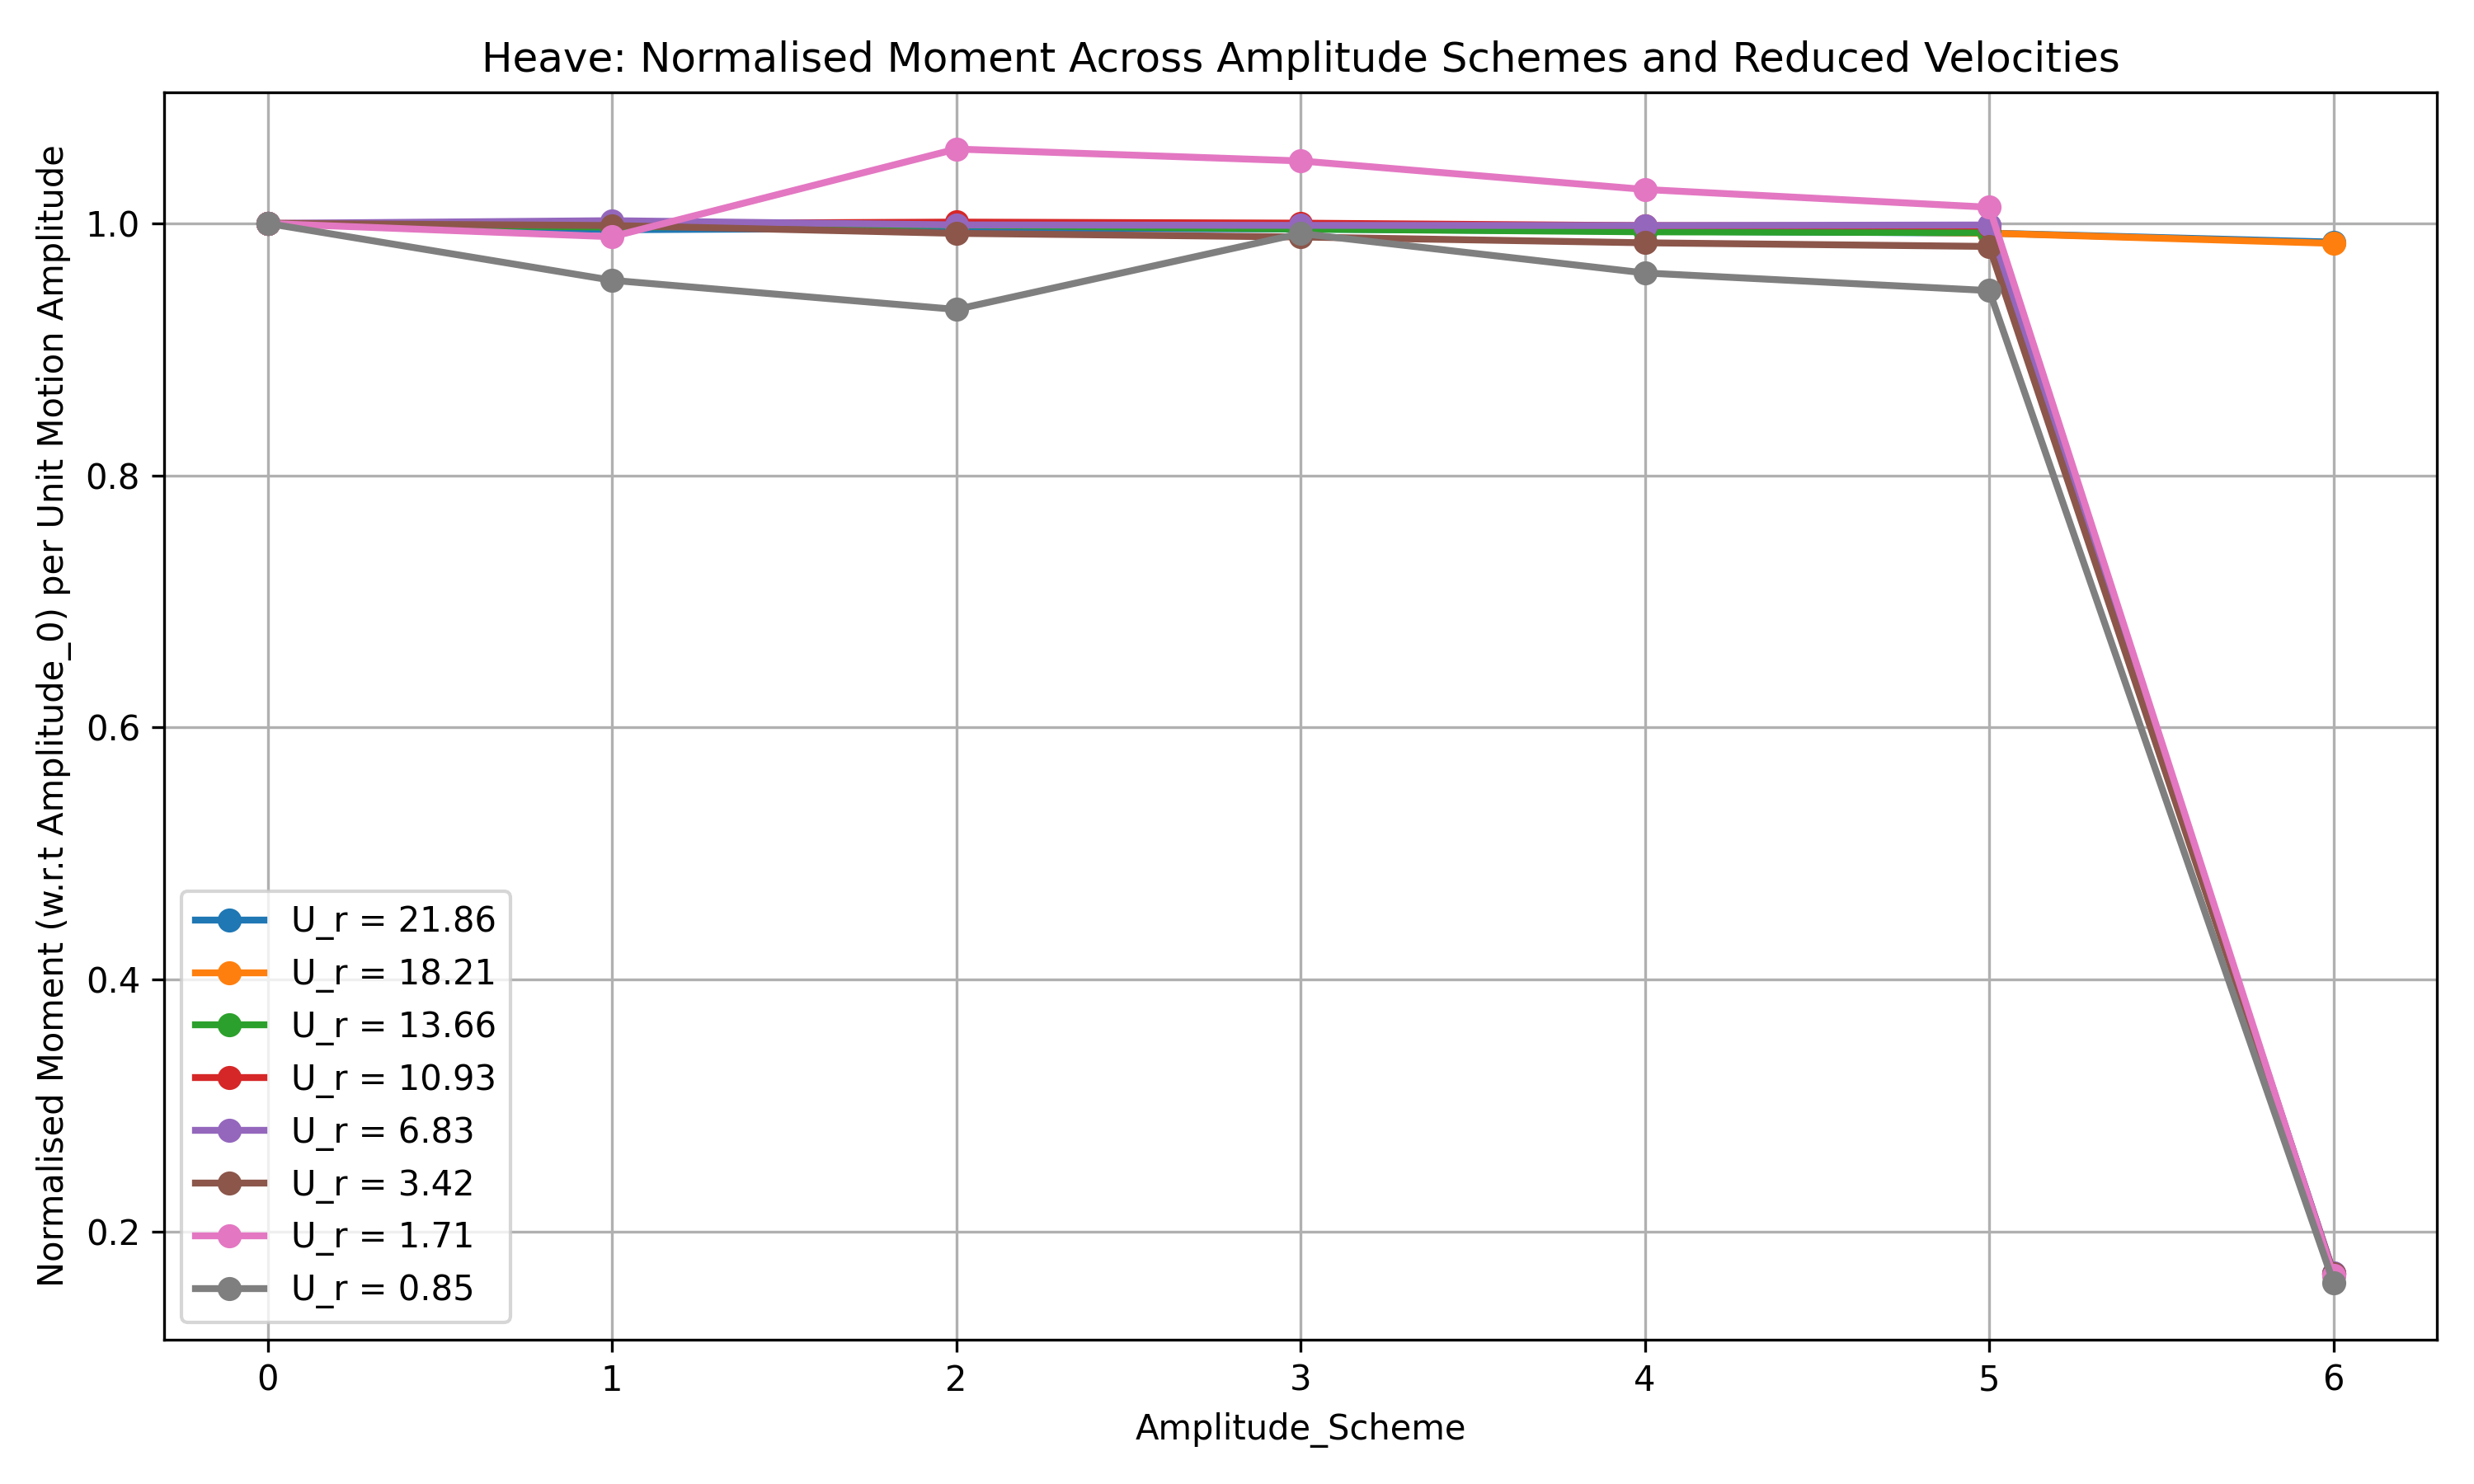
\includegraphics[width=\textwidth]{Figures/Compressed_Displacement_Vs_Force/Heave/NormalizedMoment_vs_Amplitude_Schemes_RelativeToFirst.png}
        \caption{}
        \label{fig:Compiled_Heave_Moment_vs_Amplitude}
    \end{subfigure}
    \hfill
    \begin{subfigure}[b]{0.45\textwidth}
        \centering
        
\includegraphics[width=\textwidth]{Figures/Compressed_Displacement_Vs_Force/Pitch/NormalizedMoment_vs_Amplitude_Schemes_RelativeToFirst.png}
        \caption{}
        \label{fig:Compiled_Pitch_Moment_vs_Amplitude}
    \end{subfigure}
    
    \begin{subfigure}[b]{0.45\textwidth}
        \centering
        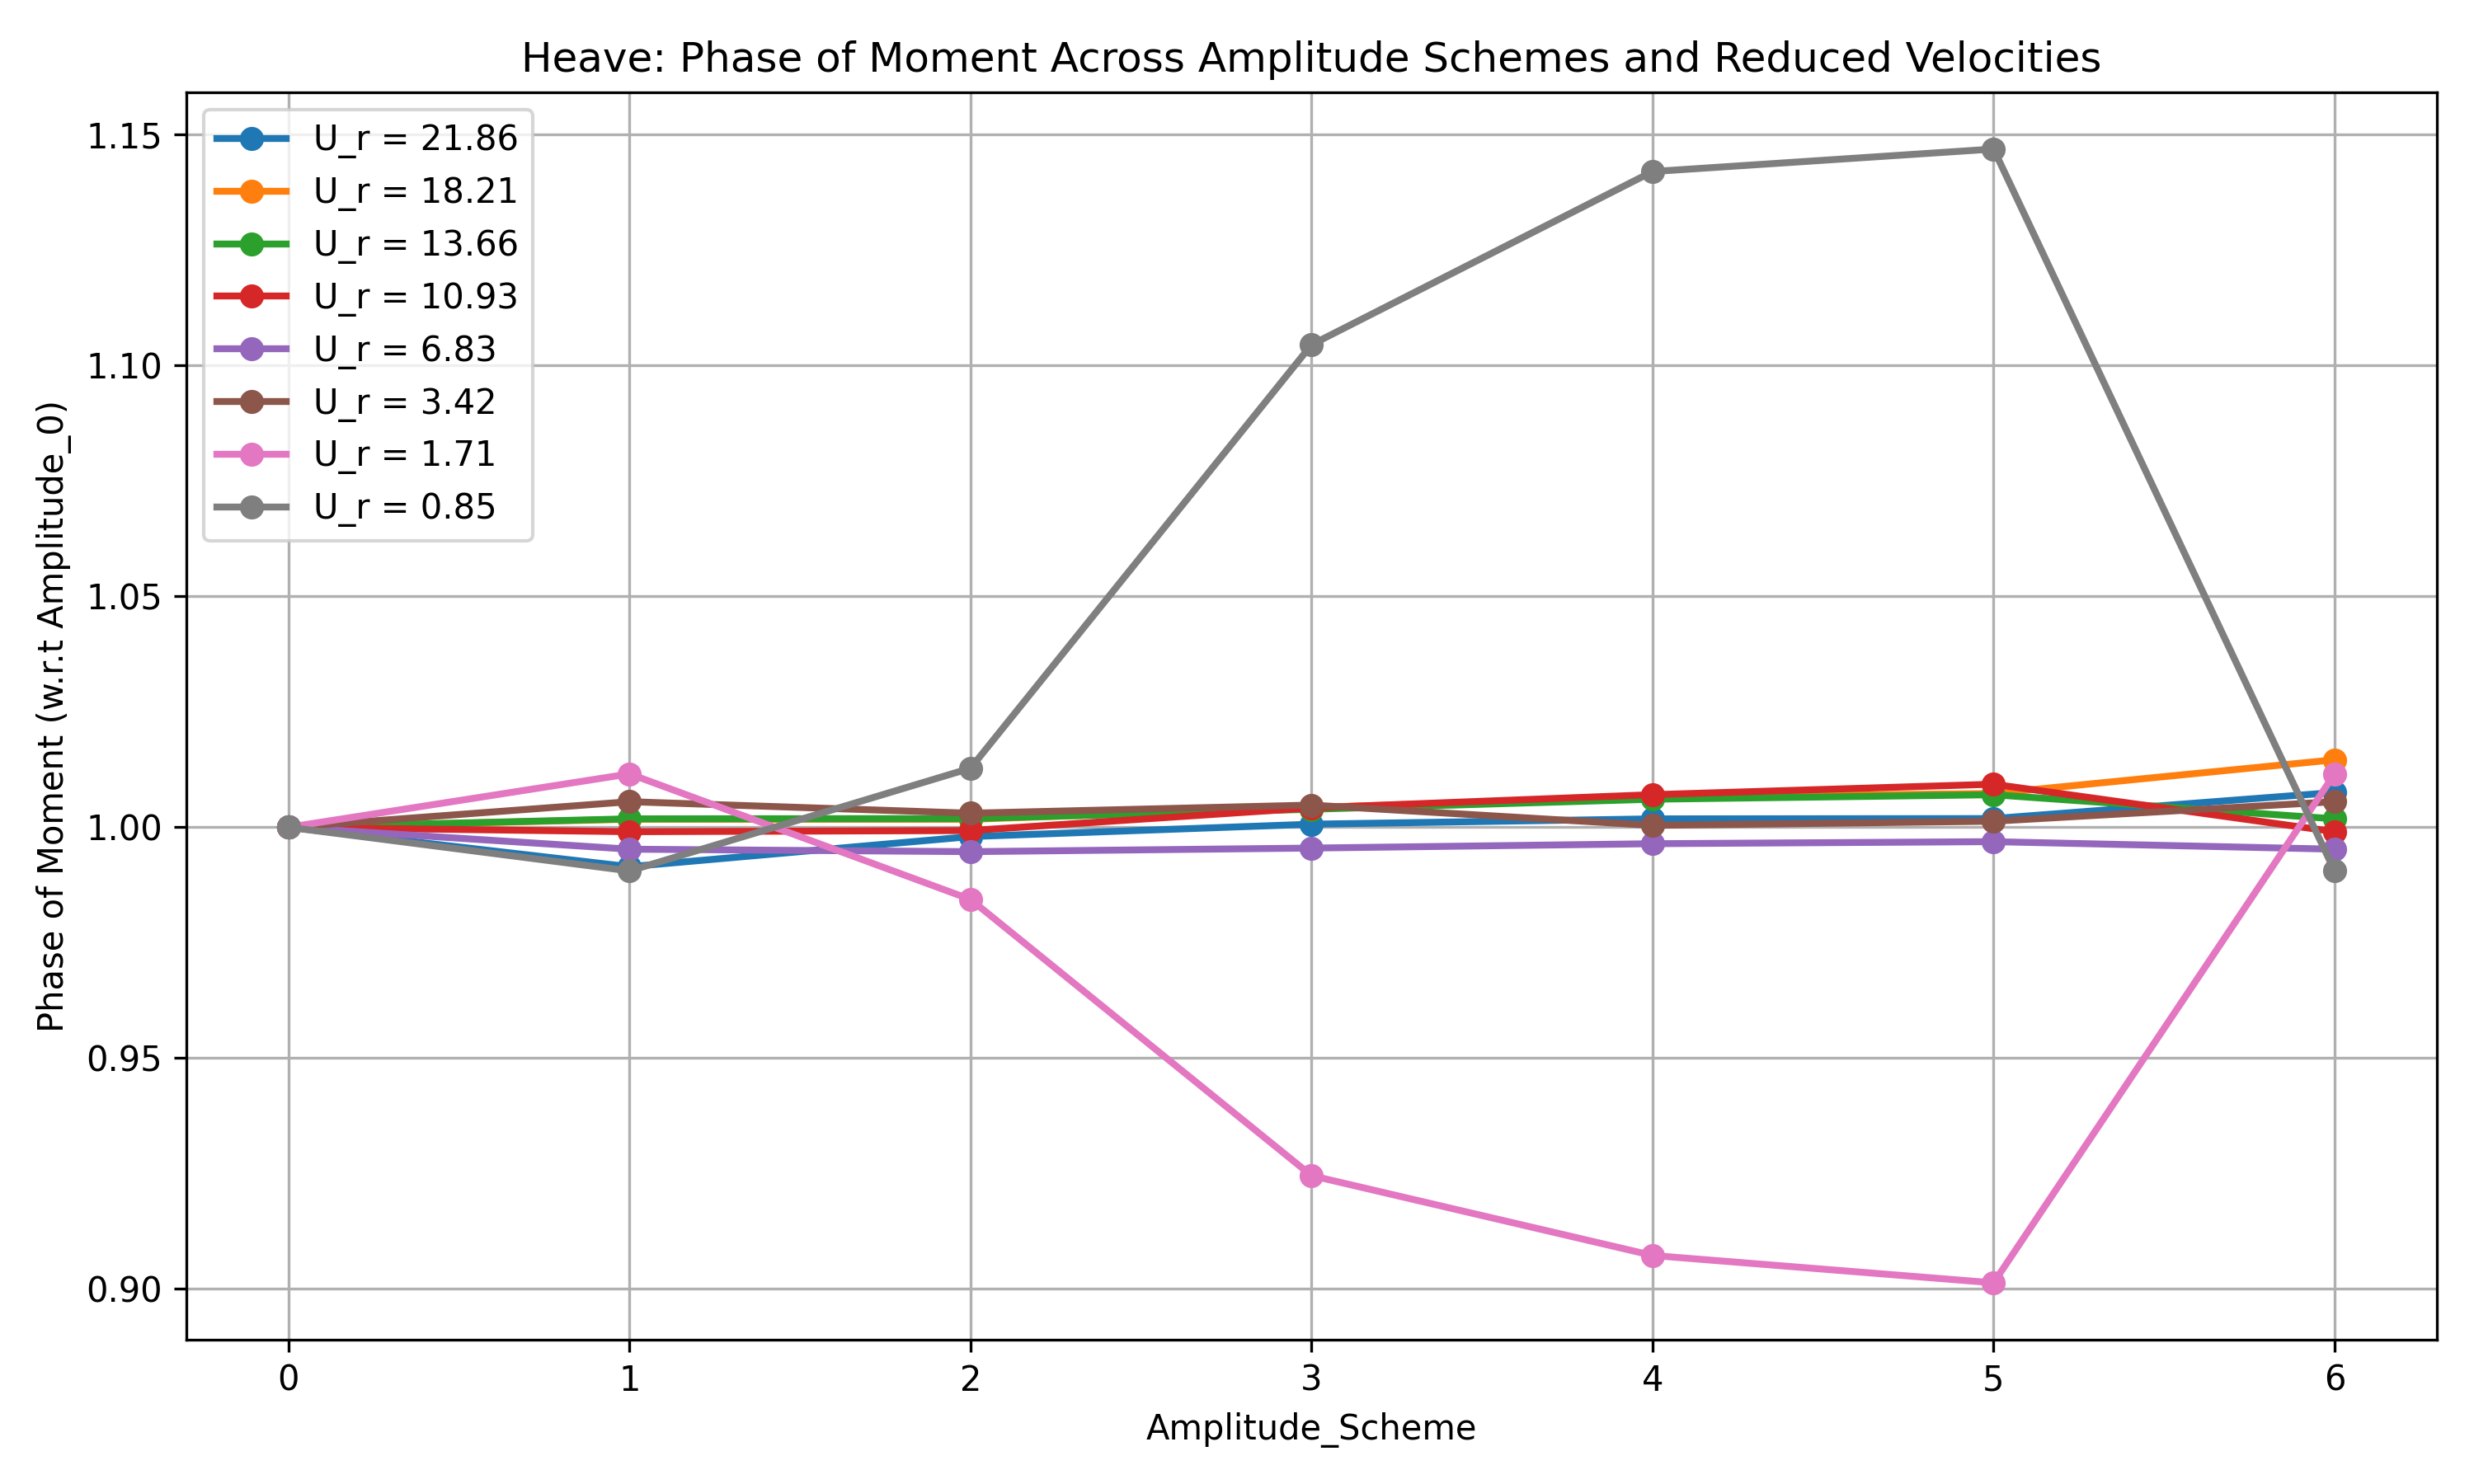
\includegraphics[width=\textwidth]{Figures/Compressed_Displacement_Vs_Force/Heave/PhaseMx_vs_Amplitude_Schemes_RelativeToFirst.png}
        \caption{}
        \label{fig:Compiled_Heave_PhaseMx_vs_Amplitude}
    \end{subfigure}
    \hfill
    \begin{subfigure}[b]{0.45\textwidth}
        \centering
        
\includegraphics[width=\textwidth]{Figures/Compressed_Displacement_Vs_Force/Pitch/PhaseMx_vs_Amplitude_Schemes_RelativeToFirst.png}
        \caption{}
        \label{fig:Compiled_Pitch_PhaseMx_vs_Amplitude}
    \end{subfigure}
    
    \caption{Compiled Prescribed Motion Displacement Vs Force}
    \label{fig:Compiled_Displacement_Vs_Force}
\end{figure}


\subsection{Pressure Distribution Analysis}

As mentioned earlier, a similar nonlinearity of derivatives $A_2$ and $H_2$ are observed by (--- and ---). 
However, in those works the nonlinearity were for a larger pitch 
angles than observed here. This difference raises the question of whether the sane underlying physical mechanism 
is responsible for the phenomenon.\\

In that paper, it has been explained that the phase shift is primarily due to changes in the flow reattachment 
point which is the result of variation in pressure distribution along the section. At small pitch amplitudes, 
the pressure field remains relatively consistent throughout the oscillation cycle. The flow around the structure does not undergo 
substantial changes between the positive and negative peaks of the pitch motion amplitude. At larger pitch amplitudes, the pressure 
distribution varies highly over the cycle because the flow field exhibits significant alterations during 
the peak pitch motion. This is the cause of observed phase deviation.\\

In order to determine whether a similar mechanism is responsible for the behaviour seen in the present study, 
pressure distributions were extracted and compared across selected pitch amplitudes. Time instants were chosen 
to cover one full oscillation cycle, starting from the negative peak displacement at 30 seconds 
(see the prescribed motion in Figure~\ref{fig:Prescribed Displacement}).\\

Figure~\ref{fig: Amplitude Study - 0 - Pitch Motion - Pressure Distribution} shows the pressure distribution 
around the cross-section at several time steps for the smallest amplitude case (Amplitude 0). The pressure field 
remains quite constant across the different phases of the motion. In contrast, for amplitude case 6 (Figure~\ref{fig: Amplitude Study - 6 - Pitch Motion - Pressure Distribution}) 
shows the pressure distribution varies highly.\\ 

Although distribution of pressure itself changes, this behaviour mainly affects the pitching moment (and therefore derivatives $A_2$ and $H_2$) 
rather than the lift force (related to $A_3$ and $H_3$). It is because, the integrated lift force remains approximately constant 
even at higher pitch angles, but the distribution of pressure on structure surface changes considerably. As a result, the effective centre 
of pressure (the moment arm weighted by the pressure distribution) shifts during the cycle, which is directly 
reflected in the pitching moment. Since the lift force is the net vertical integration, it is much less sensitive to these redistributions.\\

Finally, it should be noted that the onset of this nonlinear behaviour in pitch motion are strongly 
influenced by the breadth-to-depth ratio of the section. Hence, the amplitude threshold 
at which phase nonlinearity becomes significant will vary across different cross-sectional shapes.



\begin{figure}[htbp]  
    \centering
    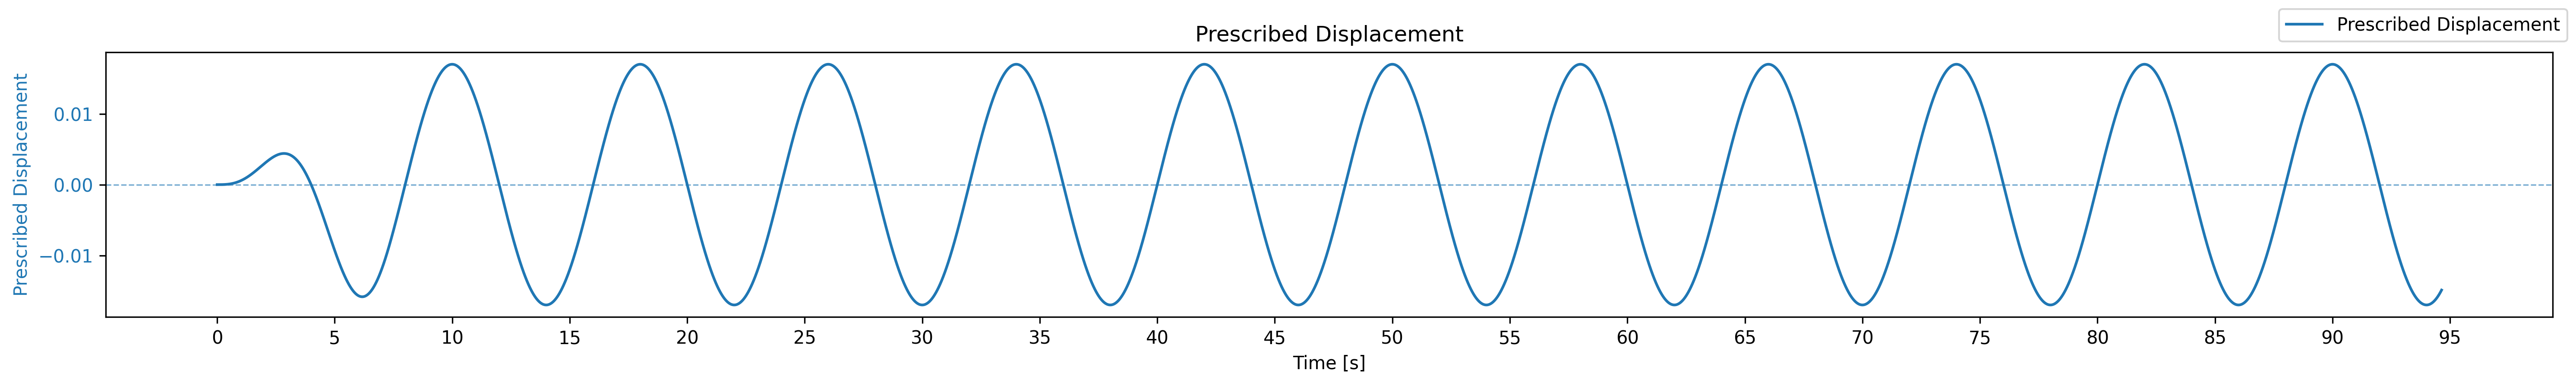
\includegraphics[width=1\textwidth]{Figures/Pitch_Study/Prescribed Displacement.png}
    \caption{Prescribed Displacement}
    \label{fig:Prescribed Displacement}
\end{figure}

\begin{figure}[htbp]  
    \centering
    \begin{subfigure}[b]{0.45\textwidth}
        \centering
        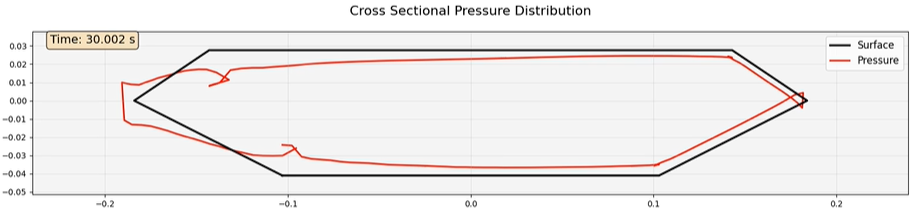
\includegraphics[width=\textwidth]{Figures/Pitch_Study/Amp_0/Amp0_Pressure_Pitch_0.125_30.png}
        \caption{Time 30 seconds}
        \label{fig: Time 30 seconds}
    \end{subfigure}
    \hfill
    \begin{subfigure}[b]{0.45\textwidth}
        \centering
        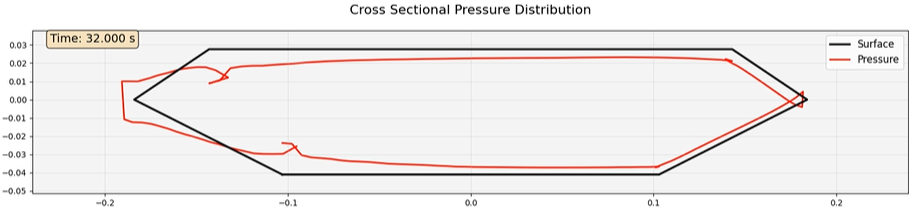
\includegraphics[width=\textwidth]{Figures/Pitch_Study/Amp_0/Amp0_Pressure_Pitch_0.125_32.png}
        \caption{Time 32 seconds}
        \label{fig:Time 32 seconds}
    \end{subfigure}
    
    \begin{subfigure}[b]{0.45\textwidth}
        \centering
        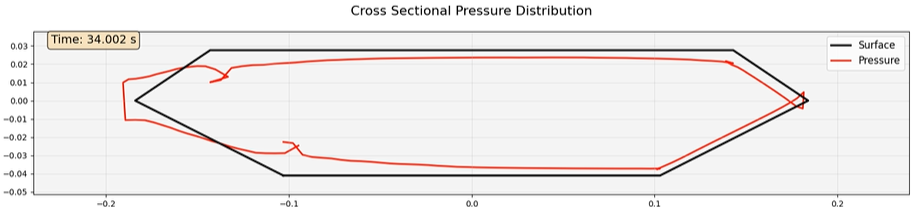
\includegraphics[width=\textwidth]{Figures/Pitch_Study/Amp_0/Amp0_Pressure_Pitch_0.125_34.png}
        \caption{Time 34 seconds}
        \label{fig:Time 34 seconds}
    \end{subfigure}
    \hfill
    \begin{subfigure}[b]{0.45\textwidth}
        \centering
        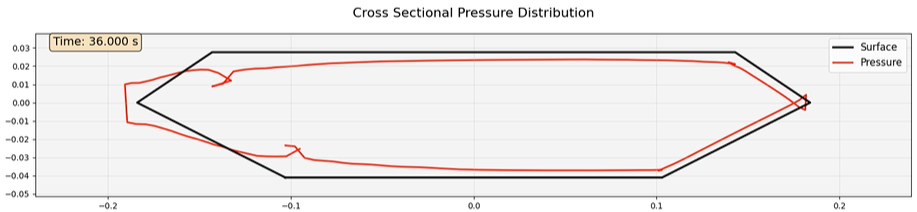
\includegraphics[width=\textwidth]{Figures/Pitch_Study/Amp_0/Amp0_Pressure_Pitch_0.125_36.png}
        \caption{Time 36 seconds}
        \label{fig:Time 36 seconds}
    \end{subfigure}
    
    \caption{Amplitude Study - 0 - Pitch Motion - Pressure Distribution}
    \label{fig: Amplitude Study - 0 - Pitch Motion - Pressure Distribution}
\end{figure}

\begin{figure}[htbp]  
    \centering
    \begin{subfigure}[b]{0.45\textwidth}
        \centering
        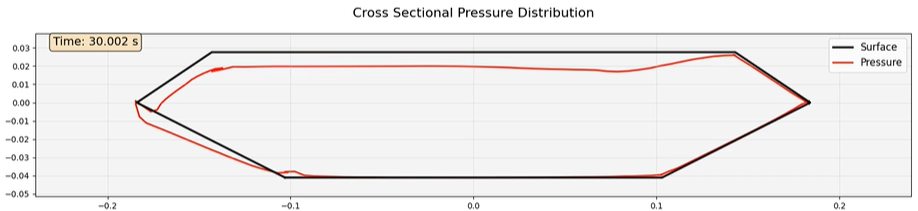
\includegraphics[width=\textwidth]{Figures/Pitch_Study/Amp_6/Amp6_Pressure_Pitch_0.125_30.png}
        \caption{Time 30 seconds}
        \label{fig: Time 30 seconds}
    \end{subfigure}
    \hfill
    \begin{subfigure}[b]{0.45\textwidth}
        \centering
        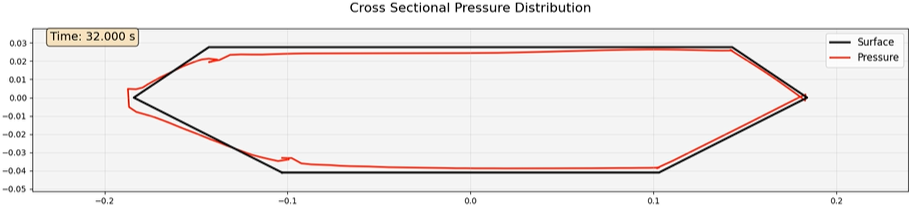
\includegraphics[width=\textwidth]{Figures/Pitch_Study/Amp_6/Amp6_Pressure_Pitch_0.125_32.png}
        \caption{Time 32 seconds}
        \label{fig:Time 32 seconds}
    \end{subfigure}
    
    \begin{subfigure}[b]{0.45\textwidth}
        \centering
        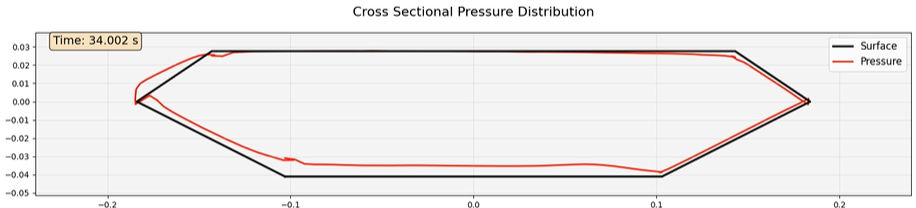
\includegraphics[width=\textwidth]{Figures/Pitch_Study/Amp_6/Amp6_Pressure_Pitch_0.125_34.png}
        \caption{Time 34 seconds}
        \label{fig:Time 34 seconds}
    \end{subfigure}
    \hfill
    \begin{subfigure}[b]{0.45\textwidth}
        \centering
        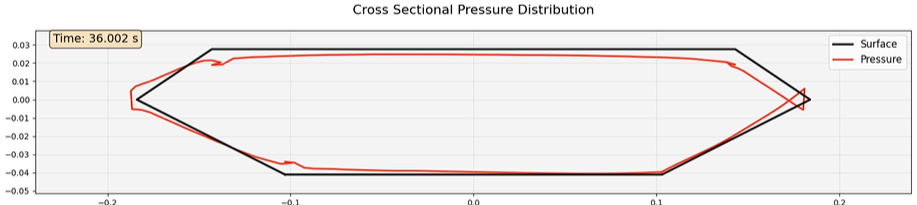
\includegraphics[width=\textwidth]{Figures/Pitch_Study/Amp_6/Amp6_Pressure_Pitch_0.125_36.png}
        \caption{Time 36 seconds}
        \label{fig:Time 36 seconds}
    \end{subfigure}
    
    \caption{Amplitude Study - 6 - Pitch Motion - Pressure Distribution}
    \label{fig: Amplitude Study - 6 - Pitch Motion - Pressure Distribution}
\end{figure}


\subsection{Influence of Nonlinearity on Critical Velocity}

Lastly, the influence of this nonlinearity on the critical velocity is studied. 
For the calculation of critical velocity, structural parameters are required. 
Structural parameters of four existing bridges are taken from - []. 
Their structural properties are summarised in Table~\ref{tab:bridge_configs}.\\

The sensitivity of the critical wind speed
to errors in flutter derivatives depends on two factors. First, whether the reduced velocity
range at which errors occur coincides with the critical flutter range of the bridge. Second,
the structural properties of the bridge determine which flutter derivative plays a dominant
role in the critical velocity prediction. To cover the second point, four structural parameters are taken.\\ 

Figure~\ref{fig:CriticalVelocity_Vs_Amplitude_Scheme} shows critical velocity obtained for all amplitude schemes. 
It shall be observed for all three bridge configurations (except Humen), till the amplitude scheme 5 there is less influence on 
obtained critical velocity. For Humen, after the amplitude scheme 3, the critical velocity varies highly. This indicates, this
bridge configuration might be more sensitive to $A_2$ and $H_2$ derivative. The reason for not observing a major deviation 
in the critical velocity (till scheme 5) is, all the critical reduced velocities are below 12 (Figure~\ref{fig:ReducedVelocity_Vs_Amplitude_Scheme} ). 
But as the errors in flutter derivatives are larger in the higher reduced velocities, 
critical velocity did not show much variations. 

\begin{table}[h!]
\centering
\caption{Structural parameters of bridge samples used for critical velocity analysis}
\label{tab:bridge_configs}
\begin{tabular}{|l|rrrrrrr|}
\hline
\textbf{Bridge} & \textbf{$B$ (m)} & \textbf{$m$ (kg/m)} & \textbf{$\zeta_h$} & \textbf{$f_h$ (Hz)} & \textbf{$I$ (kg$\cdot$m)} & \textbf{$\zeta_\alpha$} & \textbf{$f_\alpha$ (Hz)} \\
\hline
Diana (2020)       & 31.0  & 22740  & 0.003 & 0.100  & $2.47 \times 10^6$  & 0.003 & 0.278 \\
Great Belt         & 18.3  & 12800  & 0.003 & 0.1408 & $4.28 \times 10^5$  & 0.003 & 0.360 \\
% Great Belt (v2)    & 18.3  & 23687  & 0.003 & 0.097  & $2.50 \times 10^6$  & 0.003 & 0.270 \\
Humen              & 35.6  & 18300  & 0.005 & 0.1117 & $2.09 \times 10^6$  & 0.005 & 0.361 \\
Tacoma Narrows     & 11.9  & 4250   & 0.005 & 0.130  & $1.78 \times 10^5$  & 0.005 & 0.200 \\
\hline
\end{tabular}
\end{table}


\begin{figure}[htbp]
    \centering
    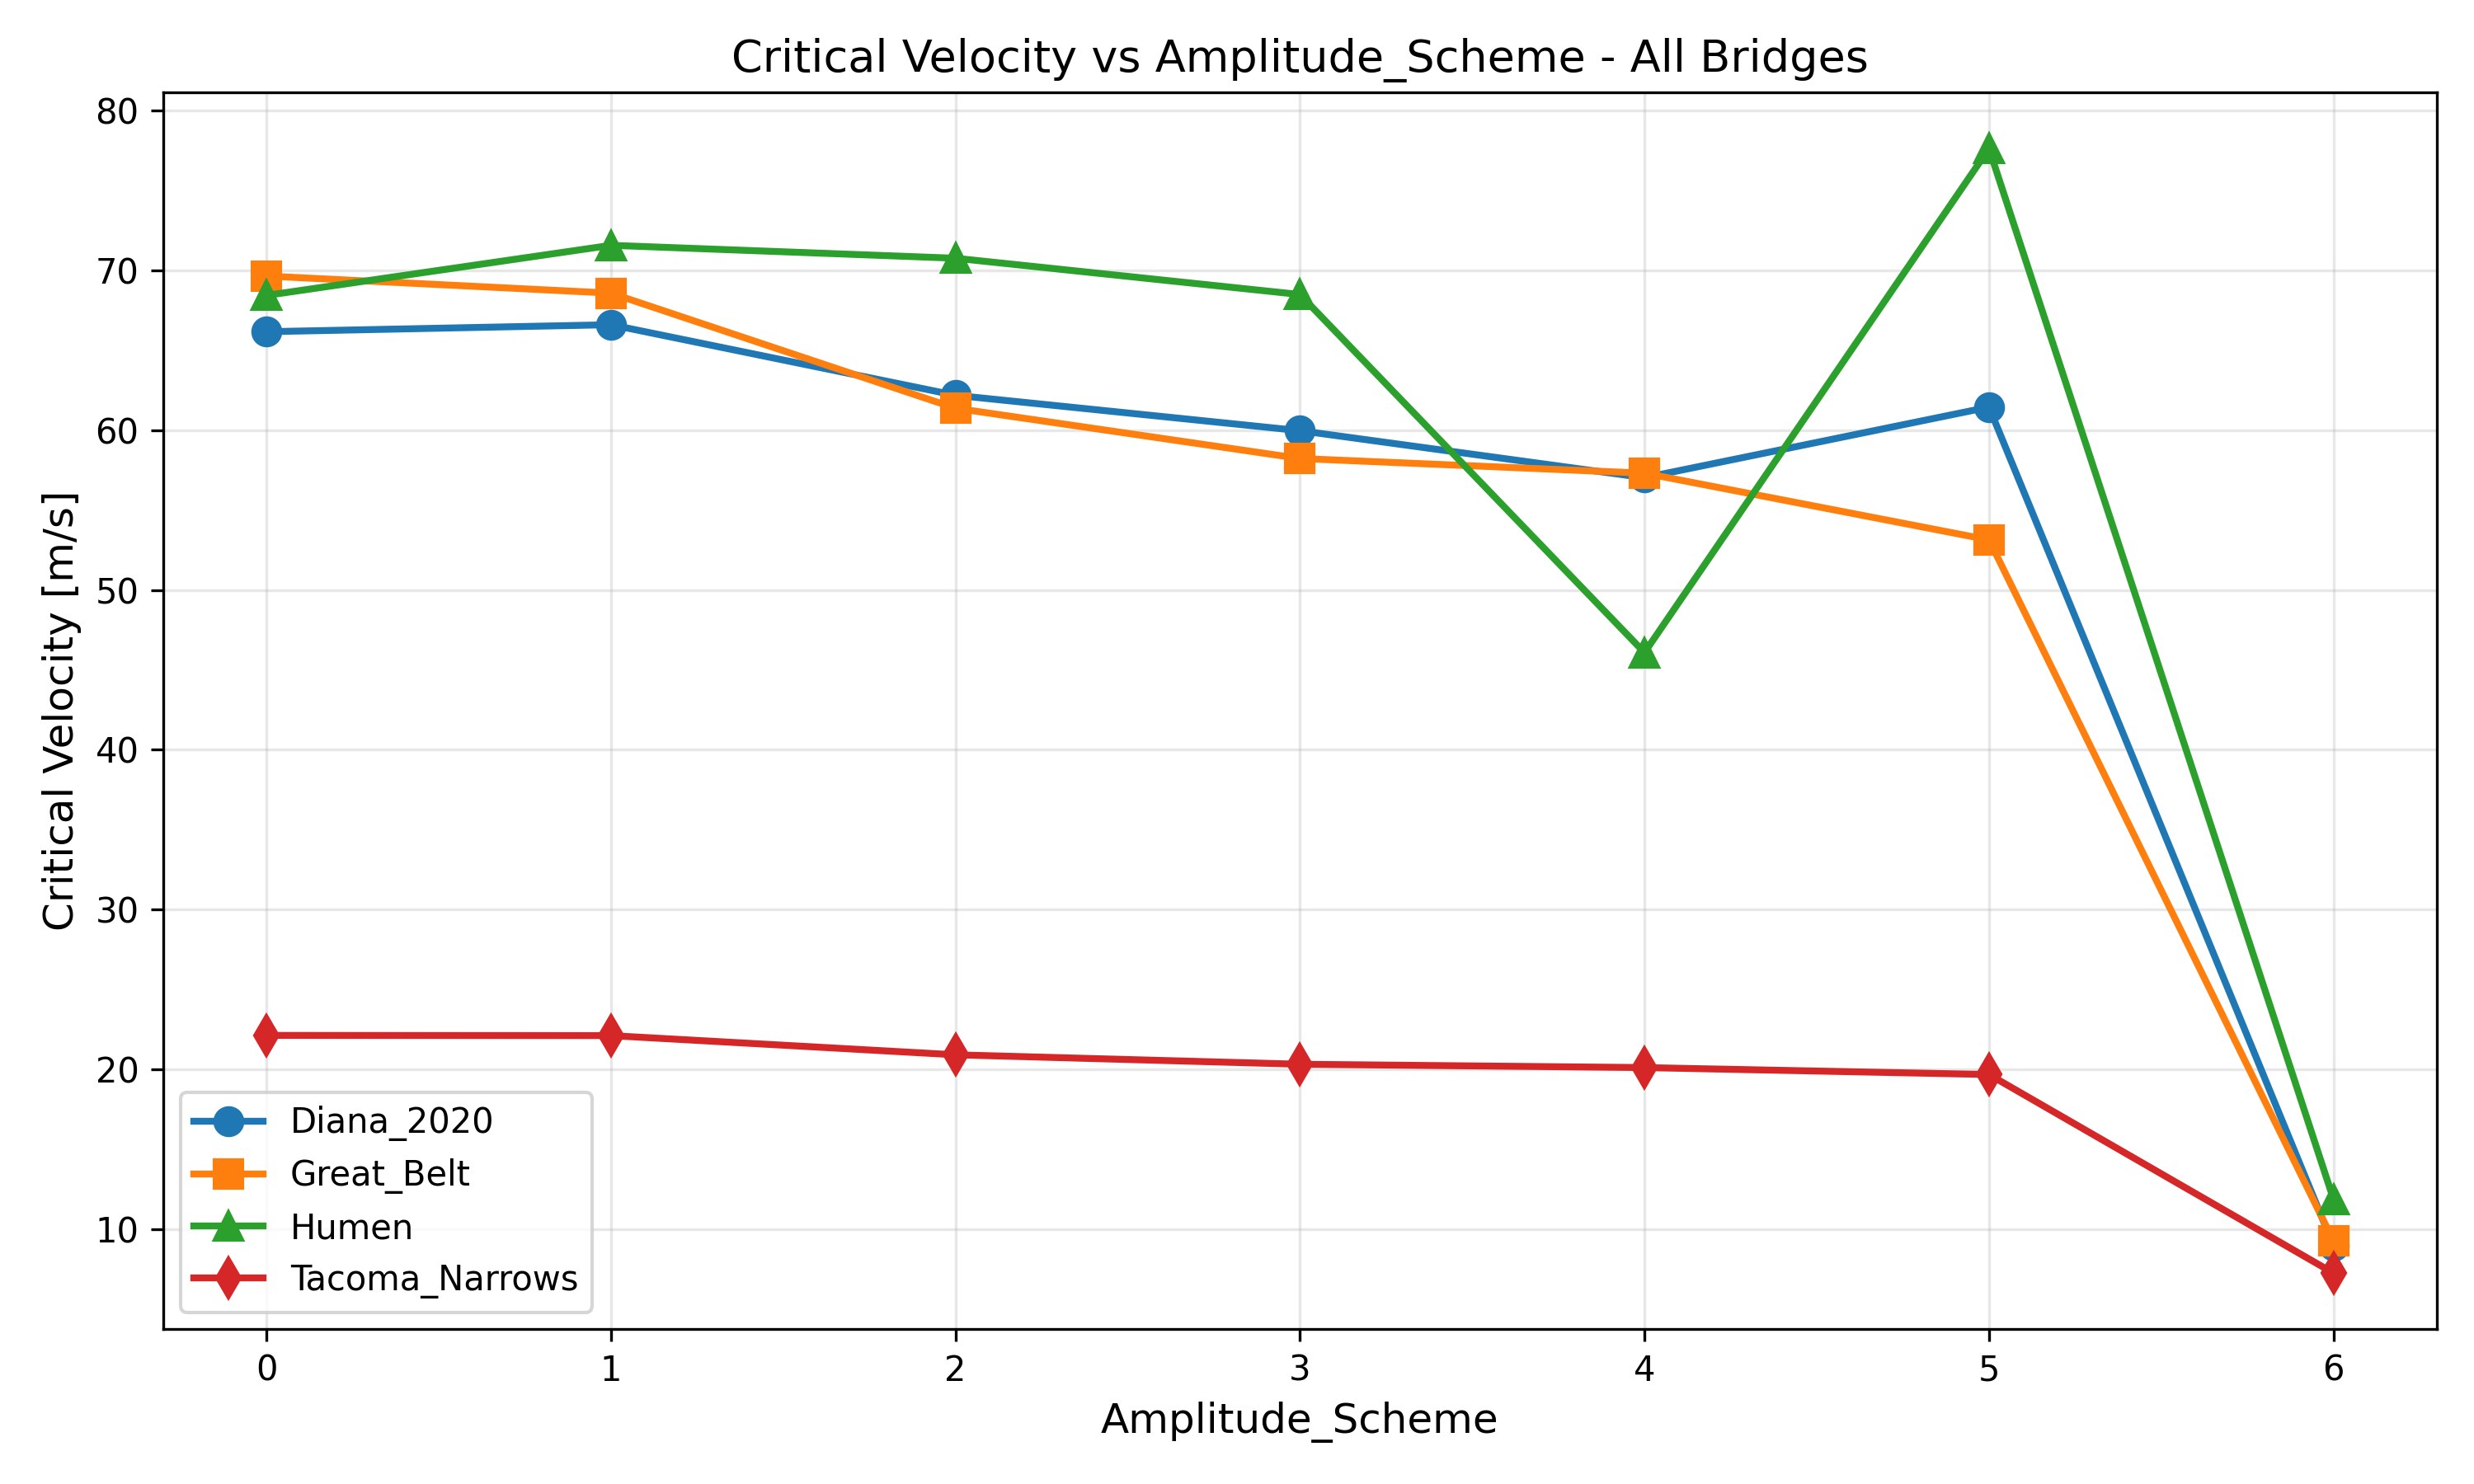
\includegraphics[width=0.75\textwidth]{Figures/CriticalVelocity_vs__Amplitude_Scheme.png}
    \caption{Critical wind speed vs.\ Amplitude Scheme}
    \label{fig:CriticalVelocity_Vs_Amplitude_Scheme}
\end{figure}

\begin{figure}[htbp]
    \centering
    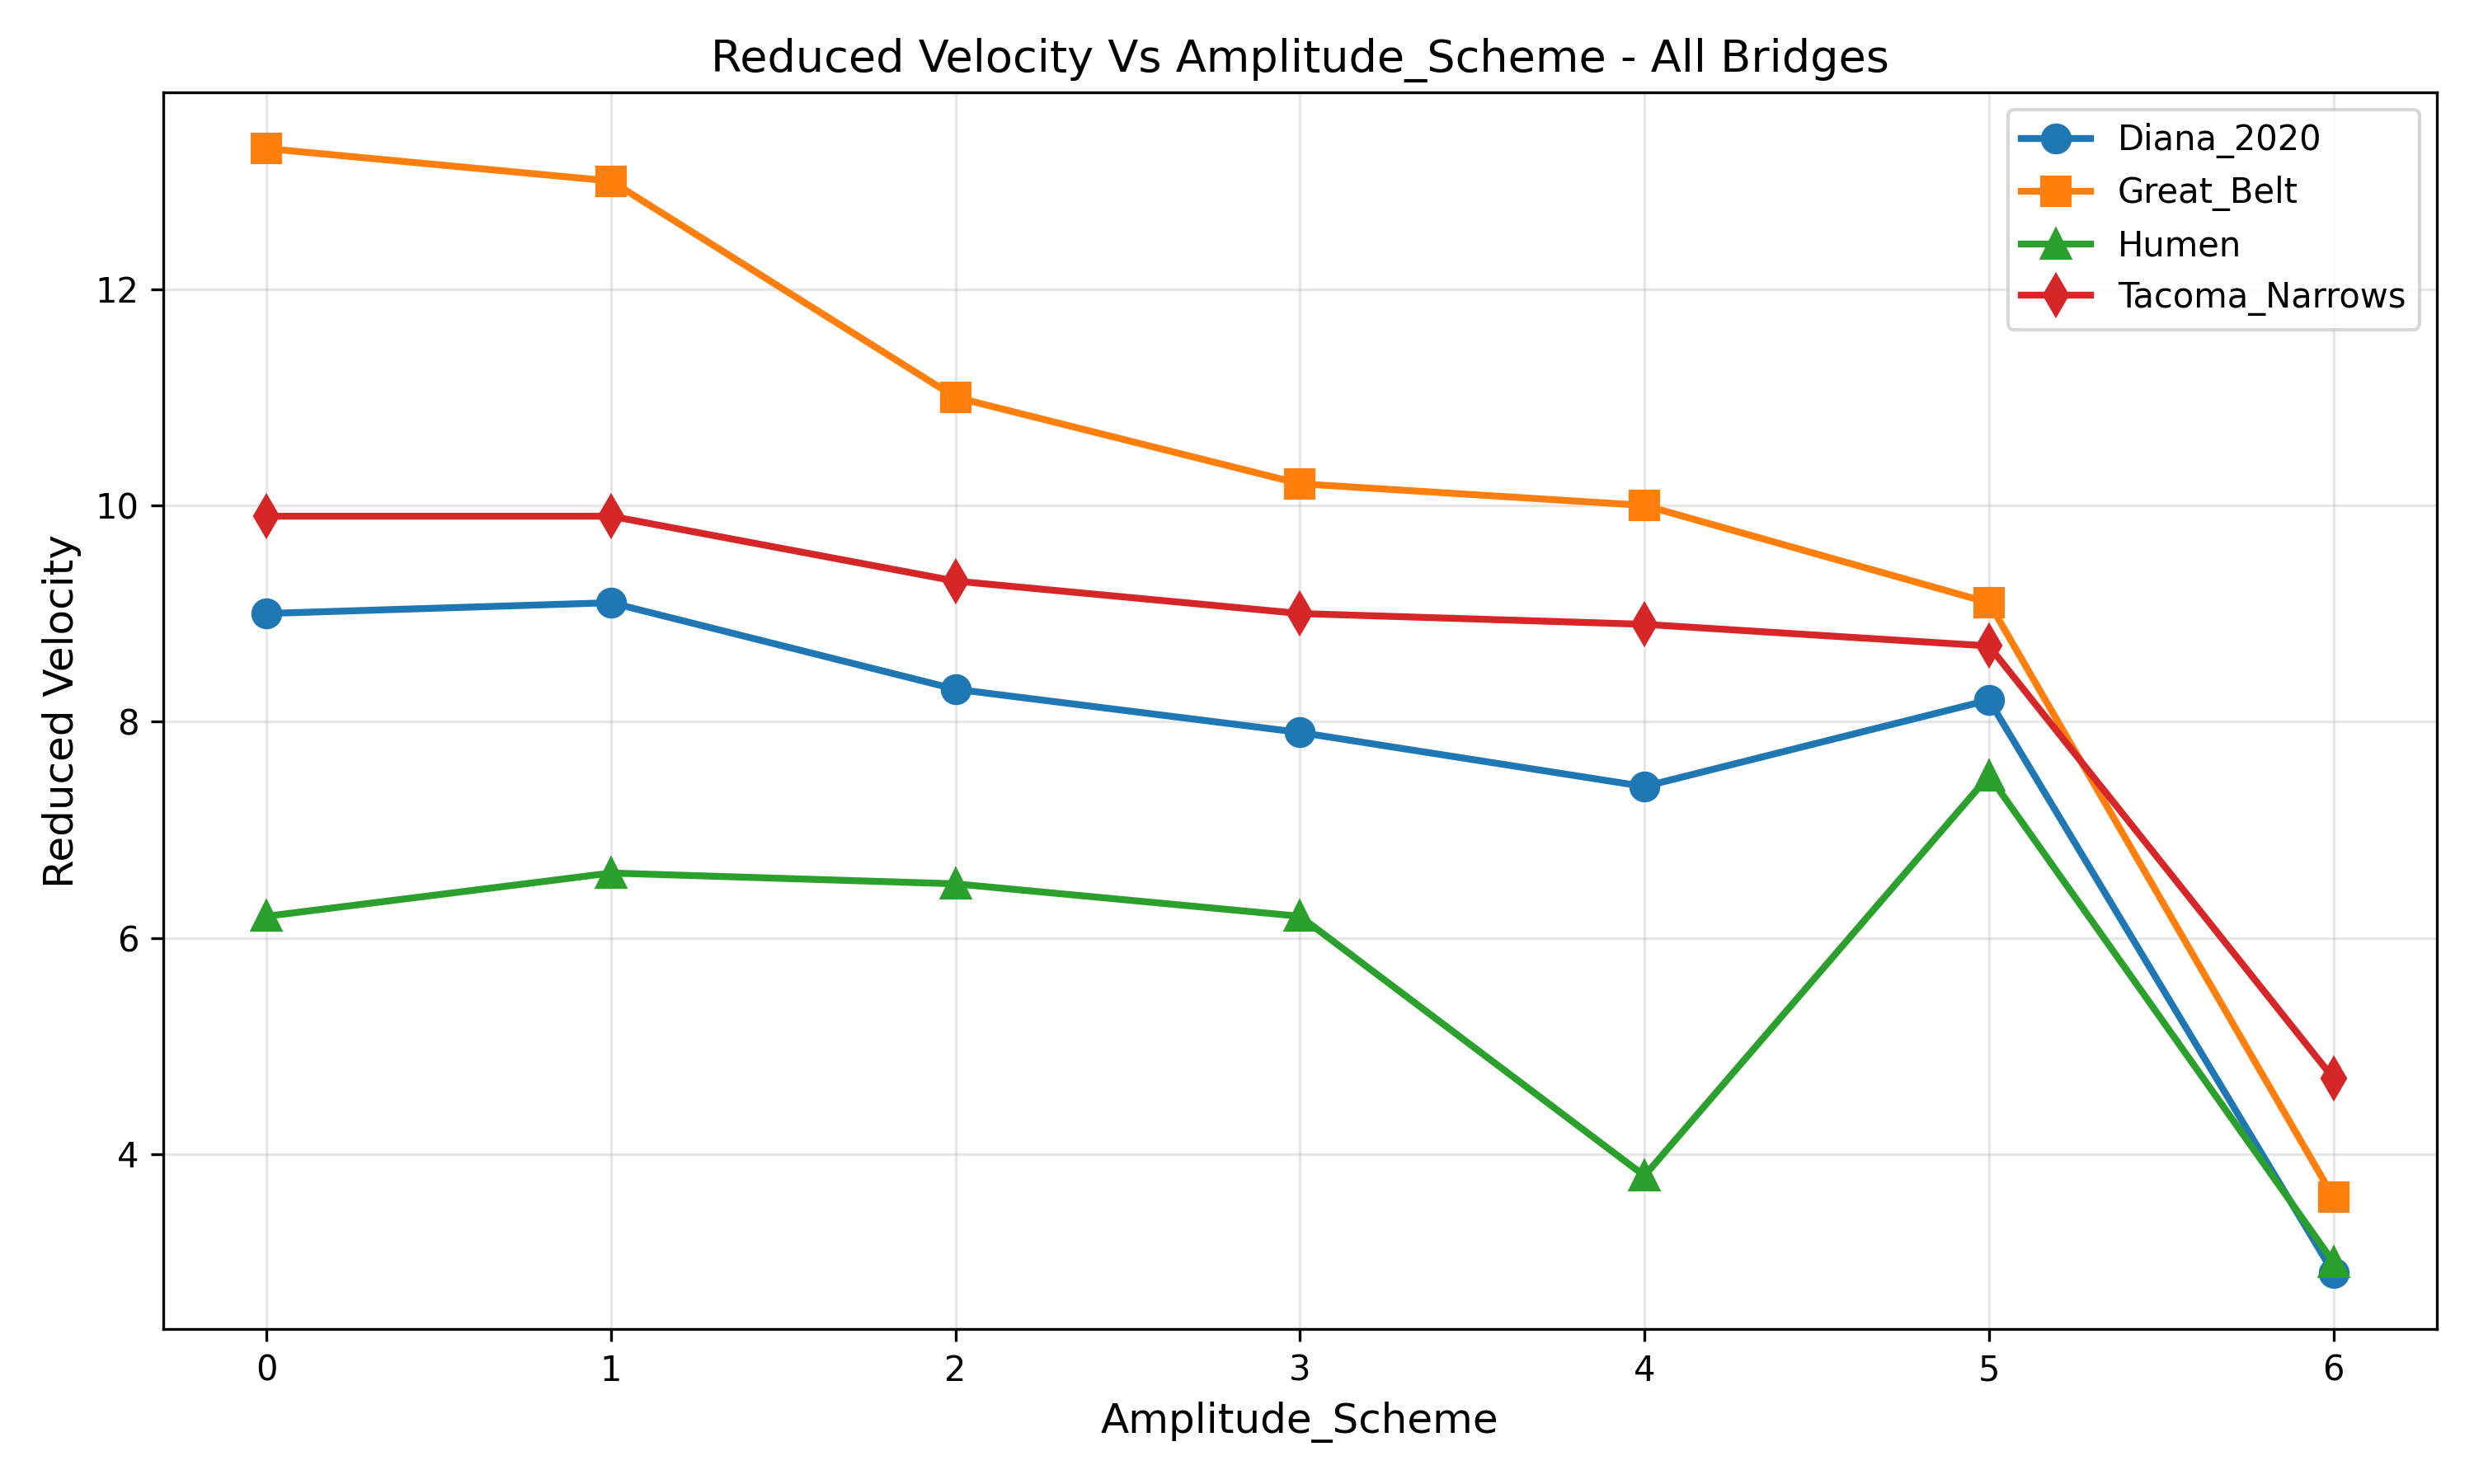
\includegraphics[width=0.75\textwidth]{Figures/ReducedVelocity_Vs__Amplitude_Scheme.png}
    \caption{Reduced critical wind speed vs.\ Amplitude Scheme}
    \label{fig:ReducedVelocity_Vs_Amplitude_Scheme}
\end{figure}

\section{Observations and Discussion}

\begin{enumerate}
    \item The linearity limit for heave motion agrees with the thumb rule; therefore, there should not be any issue with the Multi-Frequency method as long as the amplitude remains within this limit.
    
    \item Scanlan's assumptions and the principle of superposition are not equivalent and may differ; this is most clearly seen with pitch motion.
    
    \item Therefore, when validating the Multi-Frequency method, it is not necessary to obtain accurate derivatives for $A_2$ and $H_2$.
    
    \item Although the nonlinearity in $A_2$ and $H_2$ has been established in multiple research papers, the important finding here is that the present model exhibits nonlinearity at a much lower pitch degree. While the reason for this behaviour is linked to the reattachment point, an important question remains: what governs the onset of this behaviour, and why do different studies report different nonlinearity limits? This may be related to sectional properties rather than CFD modelling choices.
\end{enumerate}


\end{document}
